\clearpage
% \ifx \notincludehead\undefined
\normalsize
\end{document}
\fi


\newpage
\subsection{Управление и диспетчеризация производства}
\label{bp:production}

% На производстве работает 16 машинистов, 2 погрузчика (водителя), 1 грузчик, 1 инженер технолог, 1 инженер качества, 1 комплектовщик оснастки, 1 мастер смены.


%Производство работает в четыре смены. Смены обозначают буквами «А», «Б», «В» и «Г».

%На предприятии разработаны планы по производительности на месяц по сменам (рис. \ref{pic:f35}, \ref{pic:f36}).

\textbf{Выработка гофроагрегата}

Все задания на гофроагрегат специалист по планированию передает начальнику смены. Гофроагрегат работает только в смену с 8-00 до 20-00, но бывают исключения. Производительность гофроагрегата ограничена производительностью линий переработки. Рабочее место в пультовой сухой части гофроагрегата оборудовано ПК и принтером. Бригадир ГА получает плановое задание от начальника смены в виде файла MS Excel и распечатывает его (рис. \ref{pic:5 Задание от плановика на сухой части}). Оператор резки переносит вручную данные из планового задания в систему управления гофроагрегатом "Syncro" (рис. \ref{pic:5 Ввод в синхро}). В задании от специалиста ПП нет распределения заказов по столам, поэтому оператор на резке распределяет заказы сам в системе ''Syncro'', учитывая размеры заготовок. В случае выявления некорректных данных в задании бригадир сообщает об этом специалисту ПП по телефону или в WhatsApp. Оператор резки контролирует выполнение заказов по данным ''Syncro'' и при необходимости может скорректировать количество выпускаемых заготовок. Т.е. бригада может произвести большее количество заготовок в случае выявления брака или ''доработать'' рулон. Лишние заготовки вывозятся в цех и используются на ''нужды цеха'' или используются для выработки продукции по другим заказам. Все заготовки учтены в файле MS Excel ''НЗП'', который ведут начальники смен. В файле ''НЗП'' отражены все движения по заготовкам по всем заказам. Количество выпущенных заготовок оператор фиксирует в распечатке задания (рис. \ref{pic:4.4 задание с отметкой выработки_0001}) и в системе 1С:УПП на форме ''Рабочее место бригадира'' (рис. \ref{pic:4.2 рабочее место бригадира в УПП_0001}). После того, как будут указаны данные по количеству выпущенных заготовок бригадир не может внести корректировки и это можно сделать только через форму "Рабочее место начальника смены"(рис. \ref{pic:4.1 рабочее место начсмены в упп_0001}). Начальник смены открывает доступ бригадиру к законченному заданию и бригадир может изменить данные по выработке задания. В конце смены бригадир и начальник смены сверяют данные по выработке общаясь  по телефону или в WhatsApp. В системе ''Syncro'' фиксируются простои и бригадир или оператор резки указывают причину (рис. \ref{pic:5 Простои в синхро}). В системе ''Syncro'' существует справочник причин простоев. Информация по времени и причинам простоев передается бригадиром в конце смены начальнику смены в WhatsApp. 

Оператор на резке в системе 1С:УПП осуществляет печать ярлыков на каждую паллету (рис. \ref{pic:5.15 ярлыки с ГА_0001}) и маршрутного листа на заказ (рис. \ref{pic:5.15 маршрутный лист с ГА_0001}). Если маршрут указан неправильно, то бригадир обращается к начальнику смены и начальник смены производит со своего рабочего места печать требуемых ярлыков и маршрутных листов. Оператор на съеме контролирует высоту стоп заготовок и вносит поправки в зависимости от размеров заготовок, при этом в задании от специалиста ПП высота стопы по отдельным заказам может быть указана. Оператор на съеме вставляет ярлыки и маршрутные листы. Водитель погрузчика ориентируясь на указанный маршрут перемещает паллеты с заготовками в цех как правило ближе к указанной маршруте линии переработки (рис. \ref{pic:5 Съем заготовок с ГА}).



\textbf{Учет сырья на гофроагрегате.}

Бригада (на момент проведения аудита выполнял клеевар) исходя из площади (м2) по каждому из заданий рассчитывает необходимое количество рулонов (с учетом недомотов) и формирует заявку на сырье для кладовщика (рис. \ref{pic:5.9 заявка на сырье с ГА НА СКЛАД_0001}). Согласно заявке водитель погрузчика осуществляет подвоз рулонов на линию подачи рулонов на гофроагрегат (рис. \ref{pic:5 Подача рулонов на раскаты ГА}). На раскатах в первую очередь стараются выработать оставшиеся недомоты (рис. \ref{pic:5 недомоты у ГА}). При отсутствии необходимого сырья бригадир выполняет замену сырья по согласованию со специалистом по планированию по телефону или в WhatsApp. На мокрой части гофроагрегата установлены весы (на момент аудита отключены) (рис. \ref{pic:5 Весы на ГА}), поэтому в конце смены бригадир или клеевар замеряет диаметр, рассчитывает вес оставшихся рулонов и записывает данные в специальной форме MS Excel (рис. \ref{pic:5.14 файл бригадира по сырью_0001}). 

Начальники смен отчеты по сырью не ведут. На основании этой информации главный технолог формирует отчеты по расходу и балансу сырья. На момент аудита все рулоны, переданные на производство со склада, остаются у гофроагрегата и обратно на склад не возвращаются.  %просчитывает необходимое сырье для начала работы. Сырье на ГА доставляется грузовой машиной со склада (см. процесс "Списание сырья" \ref{bp:MatOutput}). 
%%По остаткам сырья бригадир проверяет сырье из плана. 
 
%В плане указывается резервный состав сырья. 

%План на ГА бюро планирования производства выдает в четырех экземплярах: на мокрую часть, на резки и съем. На съеме подготавливают внутренние бирки, используя картон и маркеры разных цветов. Для удобства красным цветом пишут на ящиках, черным на сложной высечке и синим на ГП (рис. \ref{pic:f21}). 

%На резках в плане указывают потоки . 
%Резчики заносят данные в систему смены заказа на автоматических резательных станках. 

%На мокрой части ГА заносят использованное сырье в отчет по расходу сырья (рис. \ref{pic:d9}), 
% \ref{pic:f21_1}), 
%которые затем передают в БППП для списания сырья. Формы отчетов расположены на каждом раскате.
%На съеме в плане оператор указывает количество произведенных заготовок. В скобках указывает  брак и количество поддонов заготовок по этому заказу. Внизу оператор подсчитывает общее количество квадратных метров. % (рис. \ref{pic:f48}). 
%Эти данные через мастера передаются в БППП в виде рапортов производства (рис. \ref{pic:d16_1}).

%На следующий день после производства инженер БППП забирает рапорта по производству у мастера, сканирует все рапорта и размещает в сетевом доступе.
%Инженер БППП заносит выработку по гофроагрегату в систему СБИС на основании рапортов гофроагрегата.
%Порядок раскроев на гофроагрегате устанавливает мастер. 
%Инженер БППП разносит выработку в систему СБИС ГА (рис. \ref{pic:d7_1}) годные заготовки. Брак не учитывается.
%Инженер БППП формирует в системе СБИС отчет производства (рис. \ref{pic:d8}).


\textbf{Выработка линии переработки}

Линии переработки работают круглосуточно. В начале каждой смены бригадир на линии переработки получает задание от начальника смены в бумажном виде. Рабочие места бригадиров оборудованы ПК и принтерами.  Бригадир в системе 1С:УПП открывает форму "Рабочее место бригадира" и находит те заказы, которые указаны задании от специалиста по планированию (рис. \ref{pic:7 рабочее место бригадира}). Бригадир при выполнении настройки на заказ вручную переносит данные ТК в панель управления (рис. \ref{pic:7 Внесение данных из ТК в программу линии}). Если заказ с печатью, то бригадир забирает подготовленные контролерами по качеству (технологами) ФПФ и краску. Штанцевальные формы бригадир берет в месте хранения у линии переработки. Бригадир в системе 1С:УПП отмечает факт выработки по каждому заказу. После того, как будут указаны данные по количеству выпущенных заготовок, бригадир не может внести корректировки и это можно сделать только через форму "Рабочее место начальника смены". 

Начальник смены открывает доступ бригадиру к законченному заданию и бригадир может изменить данные по выработке задания. В конце смены бригадир и начальник смены сверяют данные по выработке, общаясь по телефону или в WhatsApp. Бригадир фиксирует простои и в случае останова линии сообщает начальнику смены. На каждой линии ведется сменный журнал, где бригадир фиксирует выработку и информацию о работе своей смены (рис. \ref{pic:7 журнал на линии 2}). Бригадир осуществляет печать бирок на готовую продукцию по каждому заказу. Брак не фиксируется. Бракованные изделия складируются, а затем перерабатываются в макулатуру. 
После изготовления продукция поступает на транспортную линию (рис. \ref{pic:7 перемещение паллет}) и затем на паллетировку (рис. \ref{pic:7 Паллетировка}).

Начальник смены в течение смены контролирует выработку по гофроагрегату и линиям переработки и формирует бумажный отчет о почасовой выработке с указанием отставания от плановой выработки (рис. \ref{pic:4.5 почасовой отчет начсмены_0001}). Фото отчета выкладывается в группу WhatsApp. Также как и бригадиры, начальник смены фиксирует выработку по каждому заданию в бумажном варианте задания от специалиста по планированию. В конце смены данные сверяются с бригадирами. В течение смены в нескольких группах WhatsApp начальник смены ведет переписку с менеджерами, ремонтными службами и руководством. Учет рабочего времени ведется в 1С:УПП (рис. \ref{pic:4 табель смены в УПП}) и в MS Excel (рис. \ref{pic:4 рабочее время в эксель}). В конце смены начальник смены создает MS Excel документ ''Сводная ведомость'', куда вручную переносит данные из 1С:УПП по выработке заказов в течение смены (рис. \ref{pic:4.14 сводная ведомость_0001}).


Факт производства менеджеры и другие пользователи проверяют только в мессенджере Whatsapp. 
Смена закрывается в 20-00, 8-00. Бригадир отмечает выработку и фото с выработкой выкладывает в общий чат. 
Менеджер проверяет производство и факт выполнения заказа только на уровне склада по данным учета в системе 1С:УПП.



%Мастер смены получает задание на 24 часа. Распределения между линиями делает сам исходя из опыта. Мастер знает на каком оборудовании производится та или иная продукция. Также мастер ориентируется на график отгрузки. Со слов мастера бывает неравномерная загрузка по оборудованию: часть оборудования может стоять, а оставшиеся линии перегружены.
\clearpage

\begin{figure}
\begin{center}
  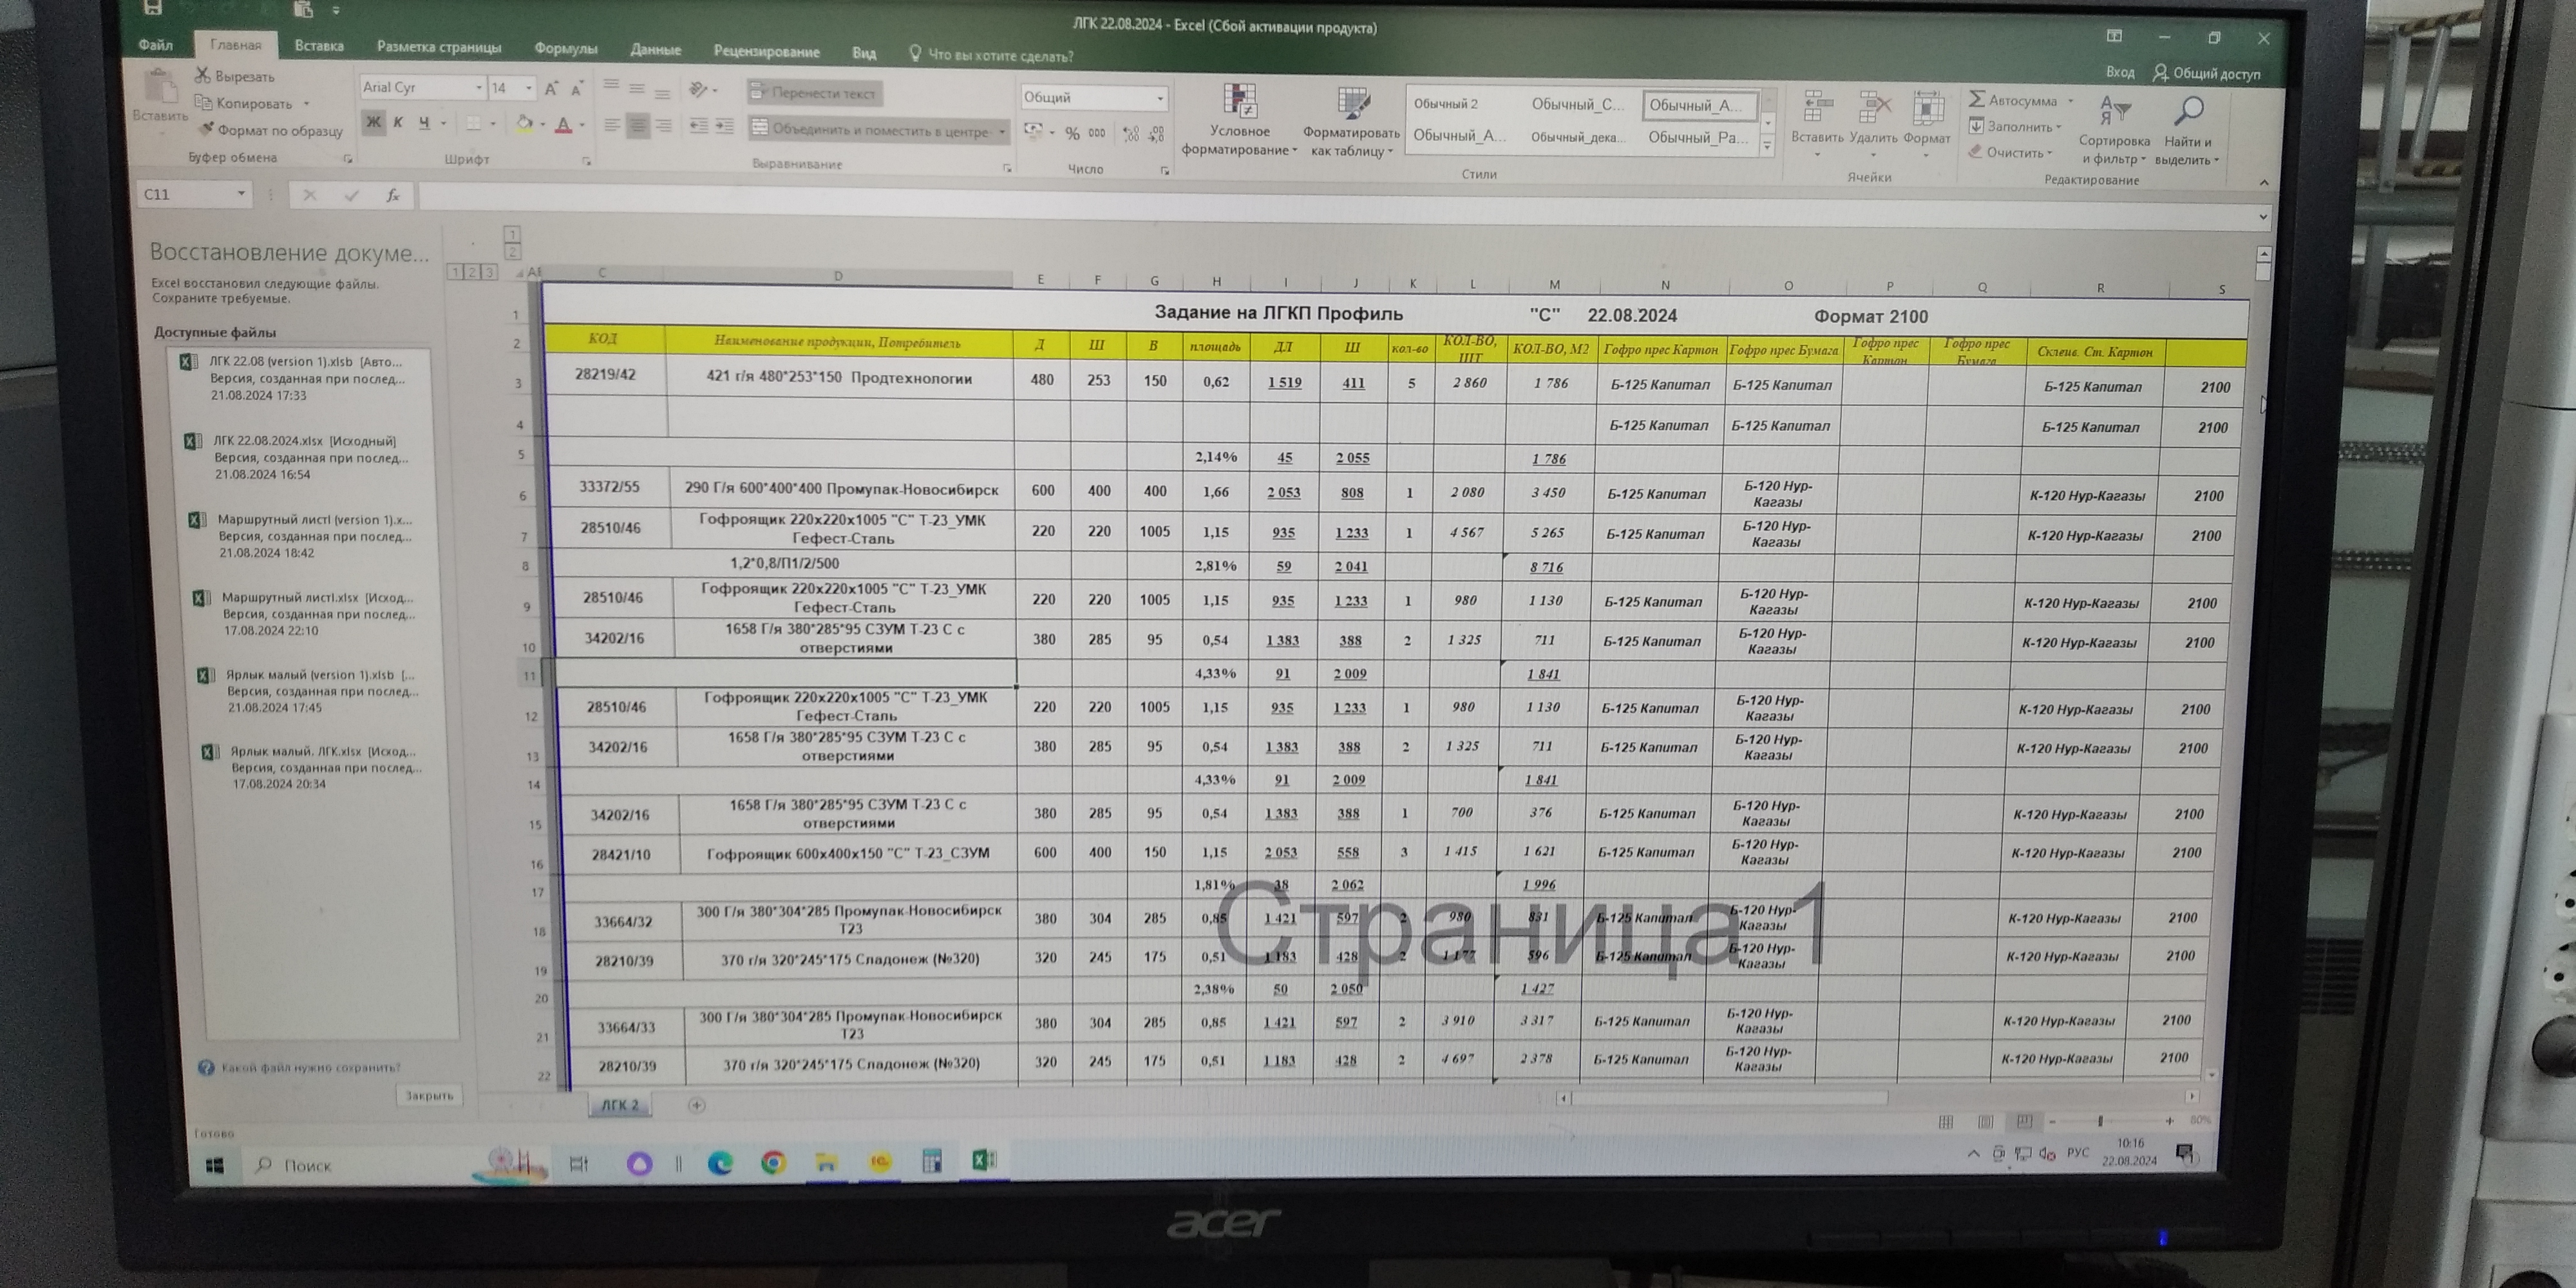
\includegraphics[height=0.94\textheight, width=0.94\textwidth, keepaspectratio]{Pics 1/5 Задание от плановика на сухой части.jpg }
\end{center}
  \caption{Плановое задание}
  \label{pic:5 Задание от плановика на сухой части}
\end{figure}

\begin{figure}
\begin{center}
  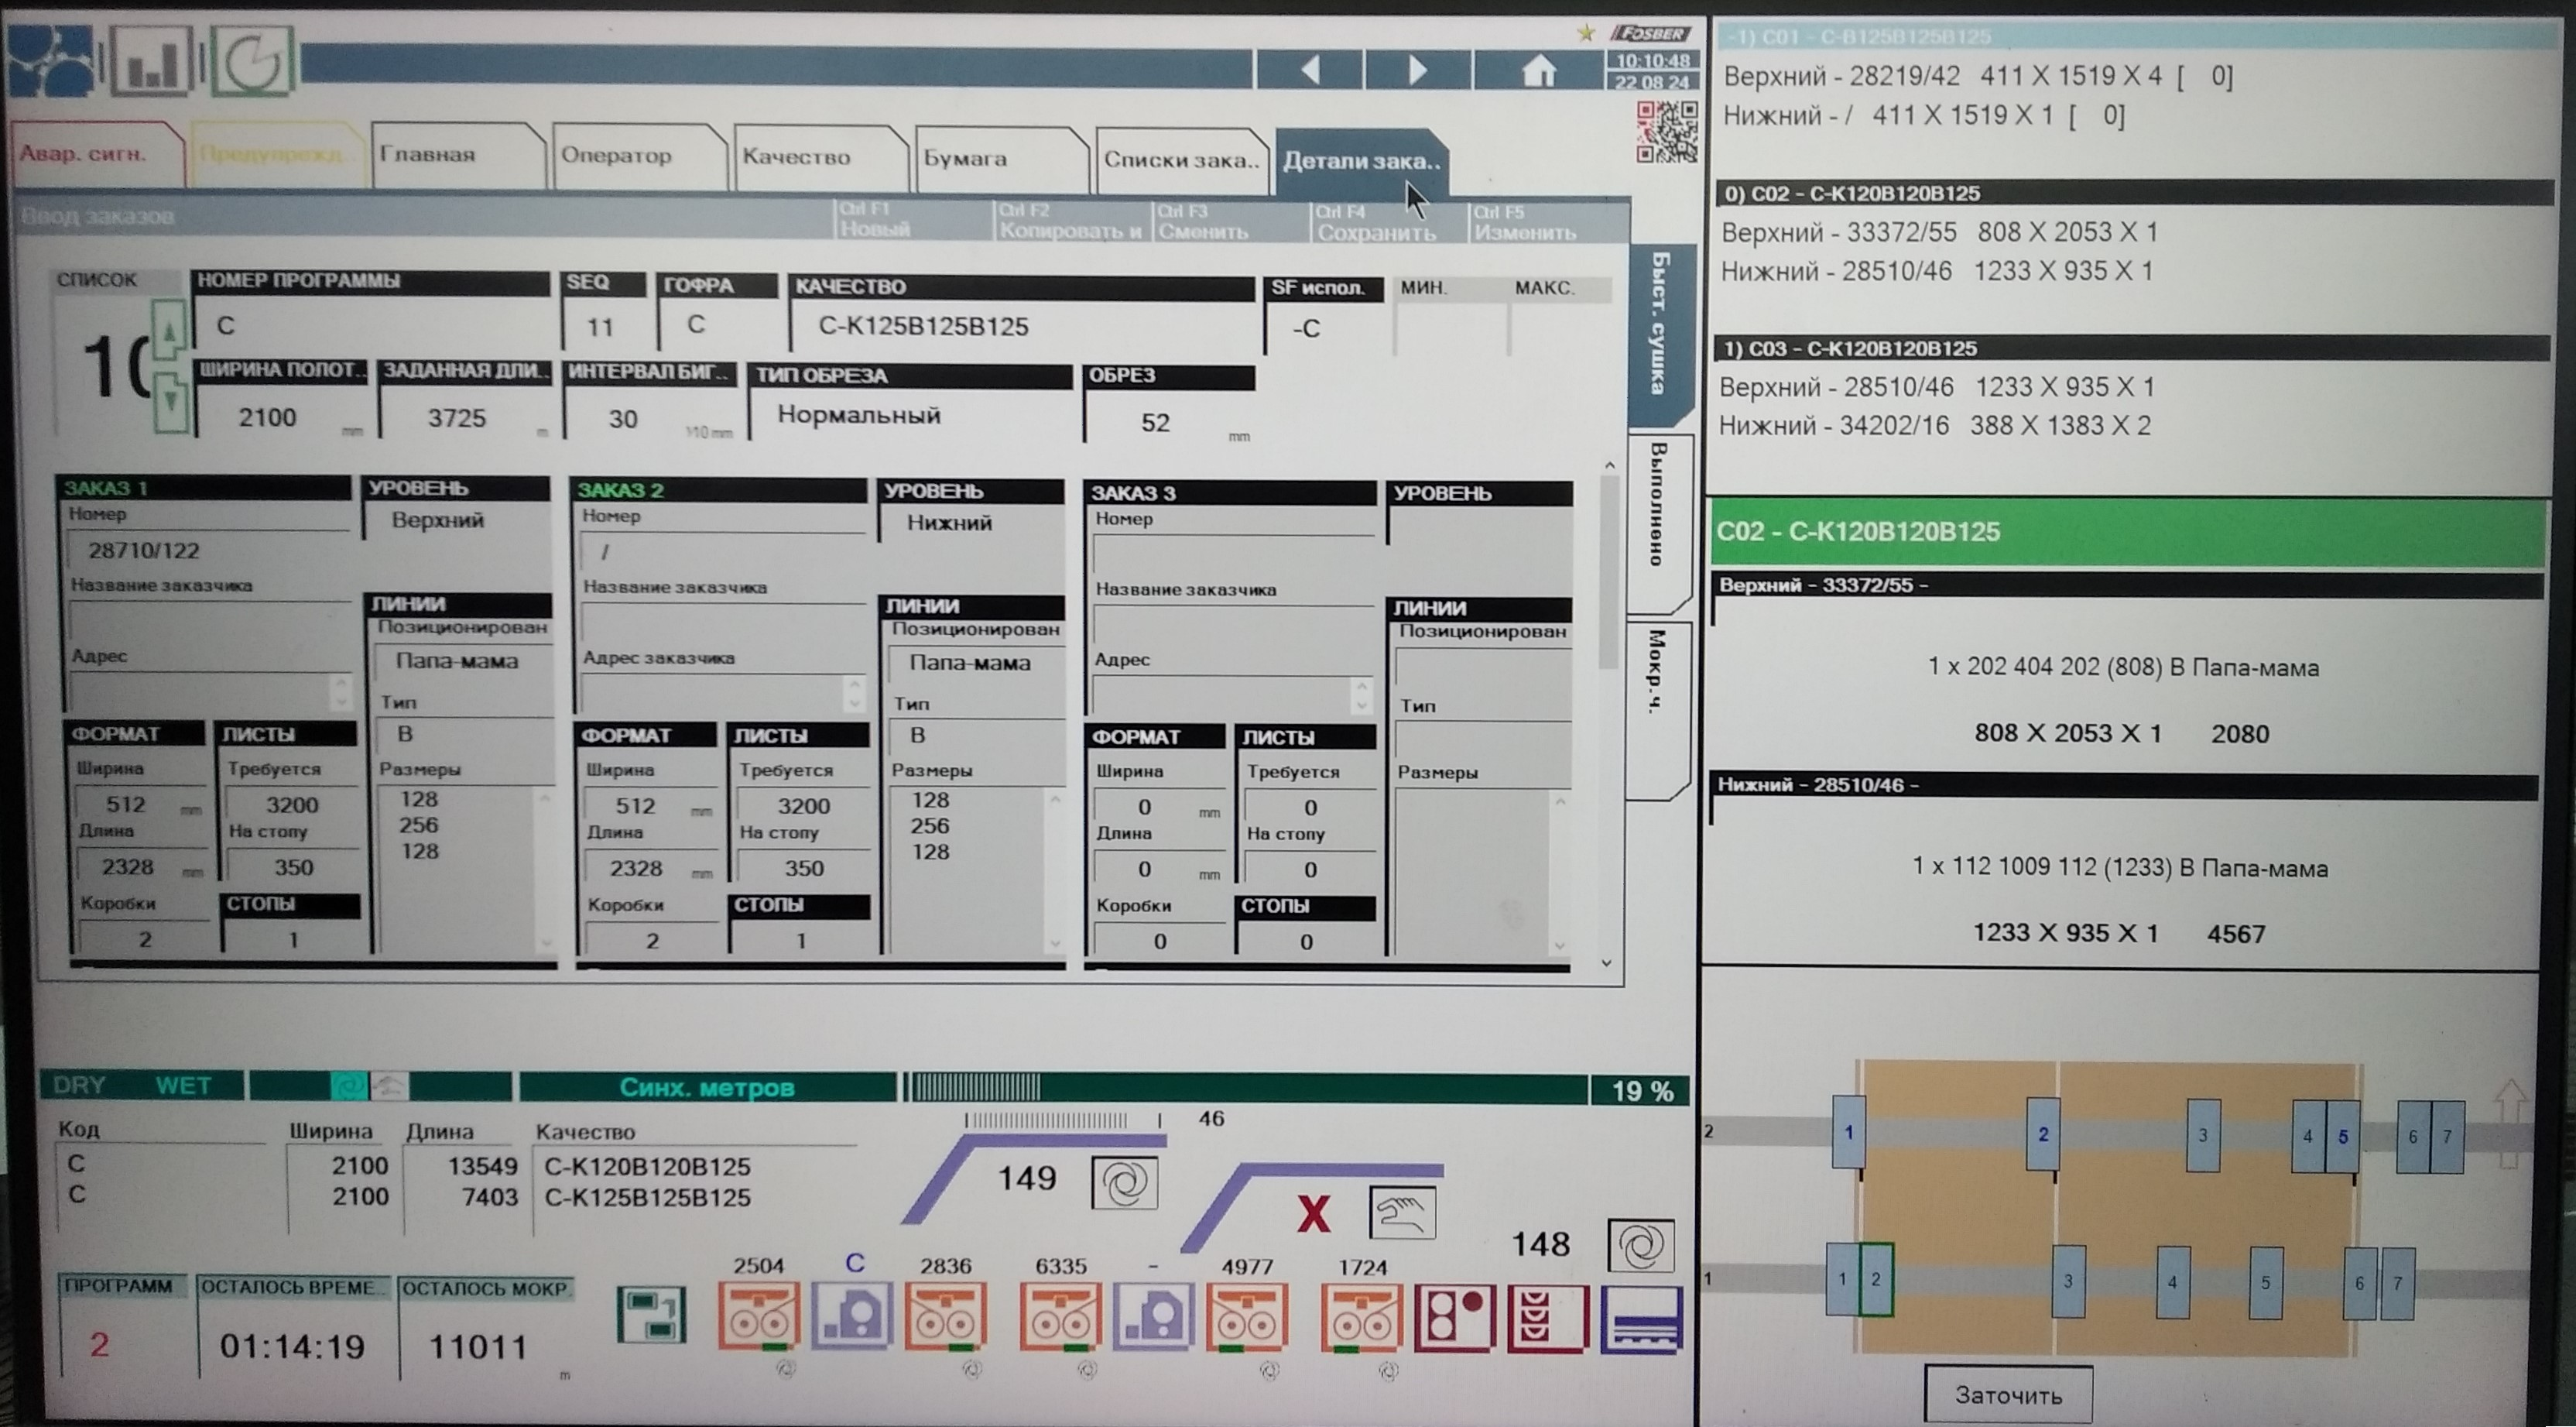
\includegraphics[height=0.94\textheight, width=0.94\textwidth, keepaspectratio]{Pics 1/5 Ввод в синхро.jpg }
\end{center}
  \caption{Внесение задания в Syncro}
  \label{pic:5 Ввод в синхро}
\end{figure}

\begin{figure}
\begin{center}
  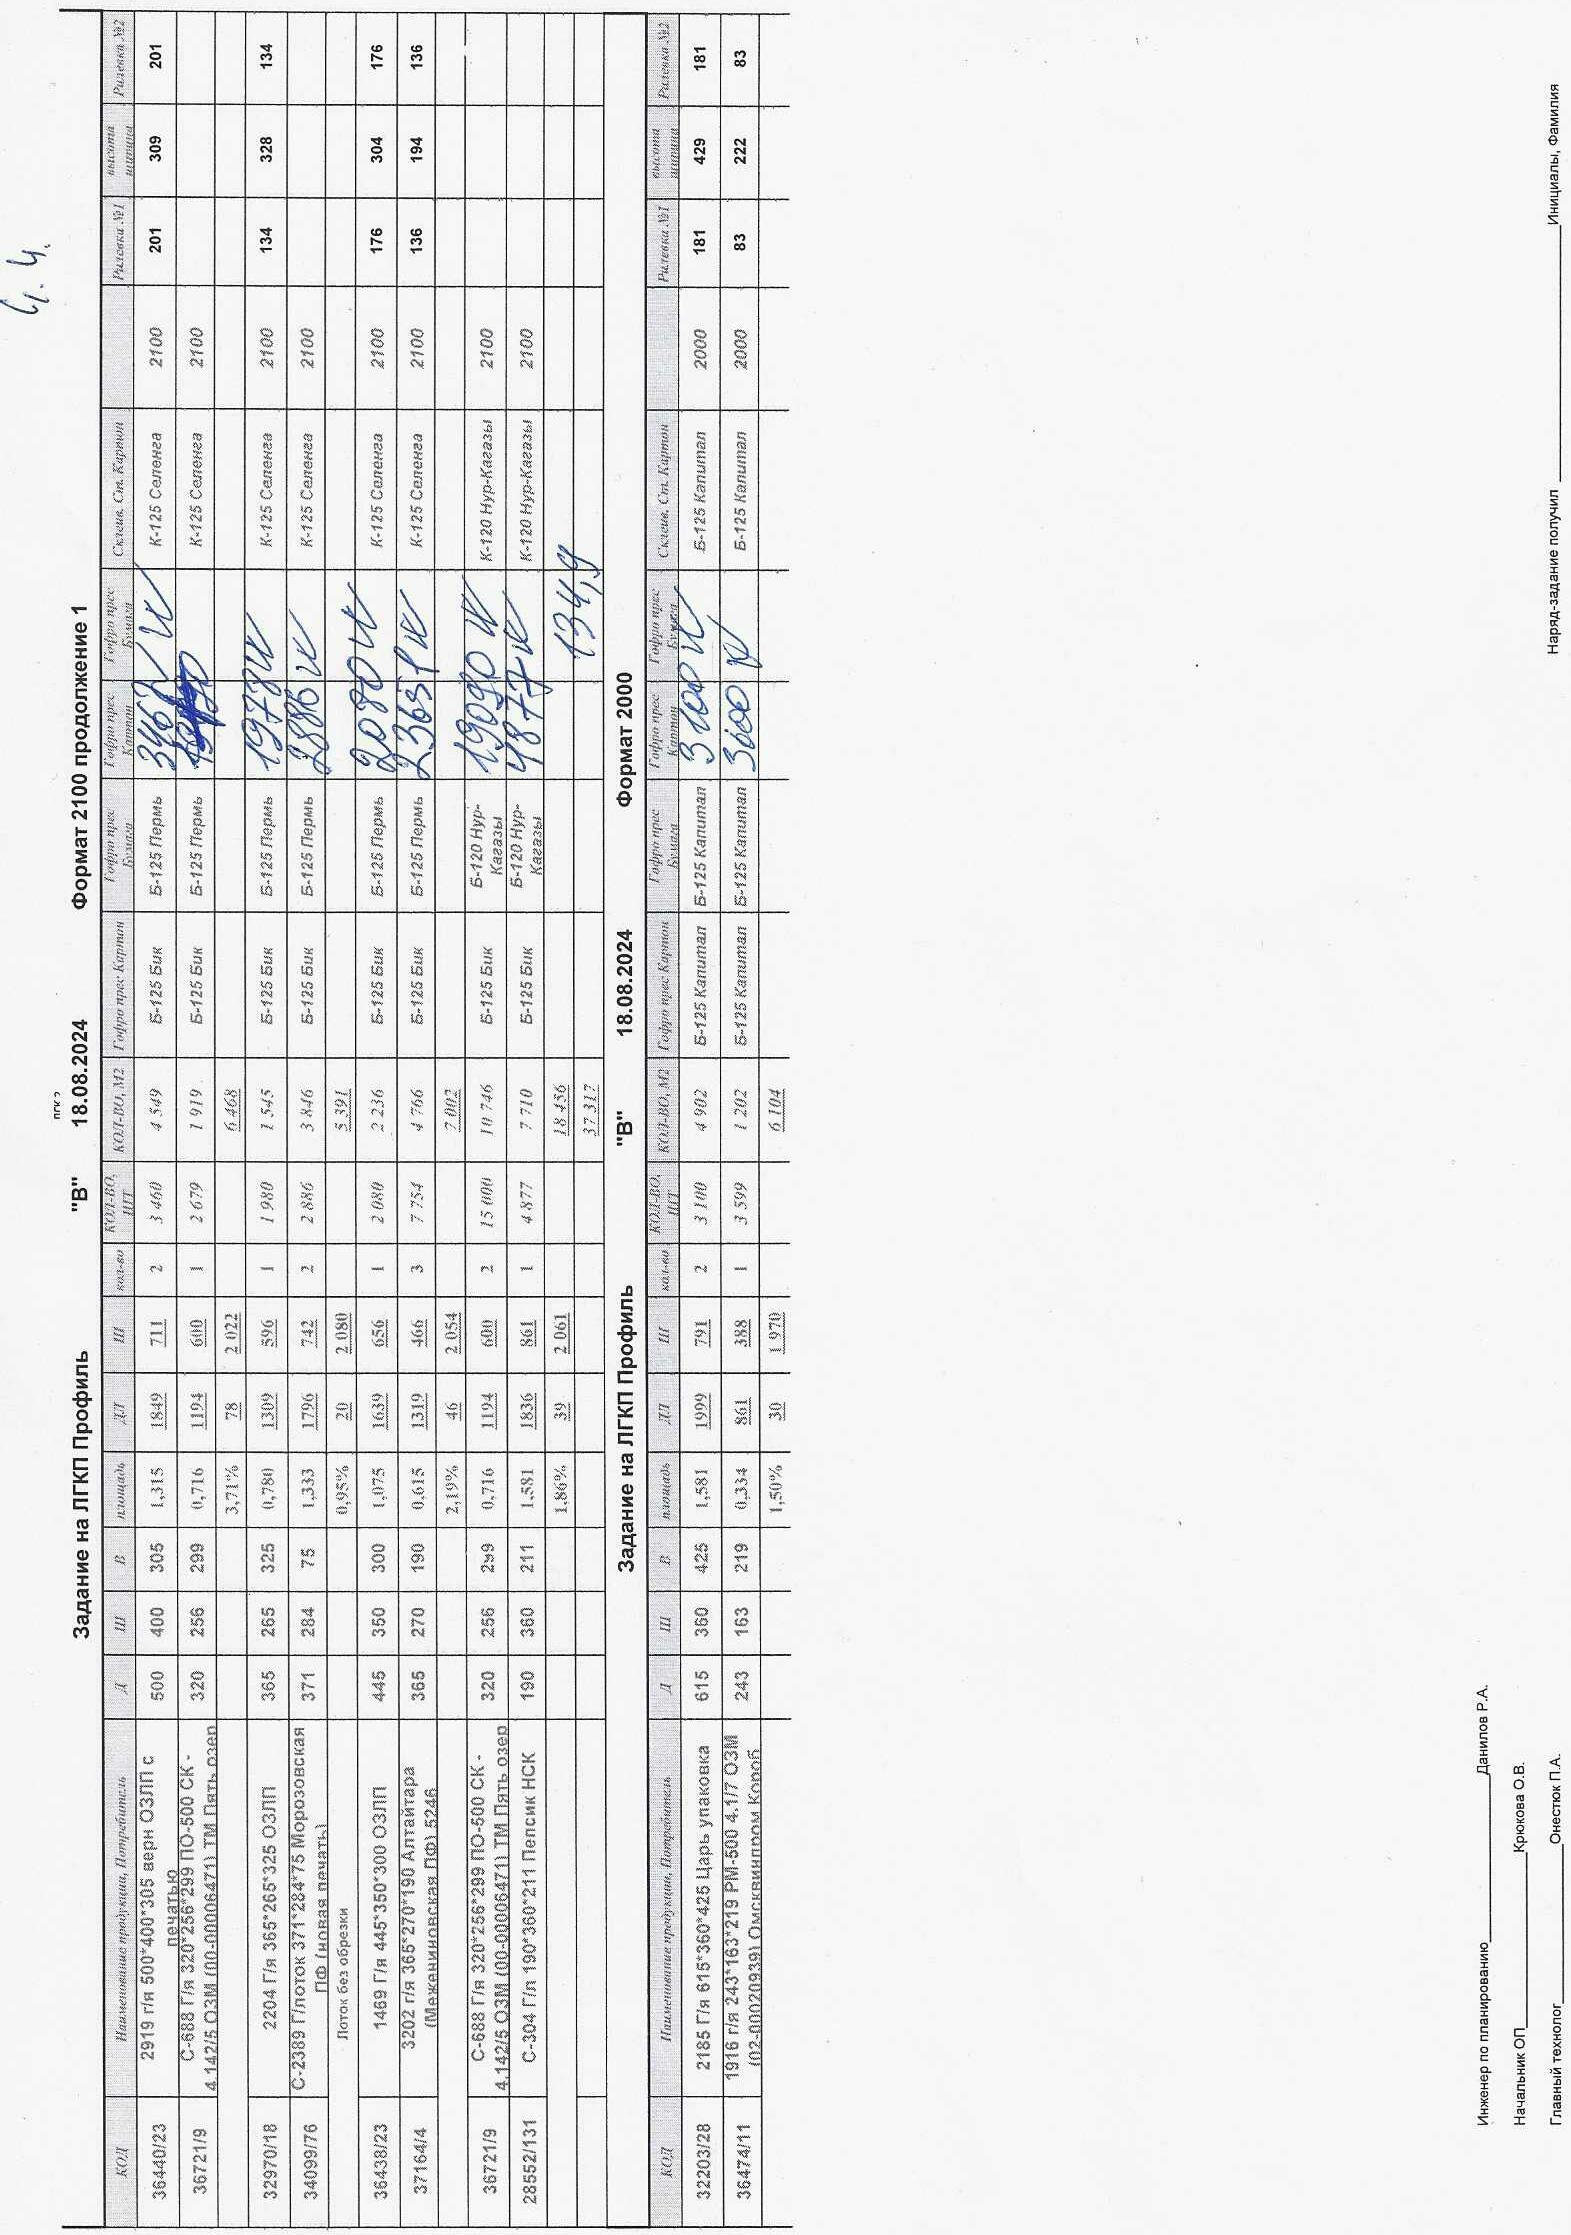
\includegraphics[height=0.94\textheight, width=0.94\textwidth, keepaspectratio]{Pics 1/4.4 задание с отметкой выработки_0001.jpg}
\end{center}
  \caption{Задание с отметками о выработке}
  \label{pic:4.4 задание с отметкой выработки_0001}
\end{figure}

\begin{figure}
\begin{center}
  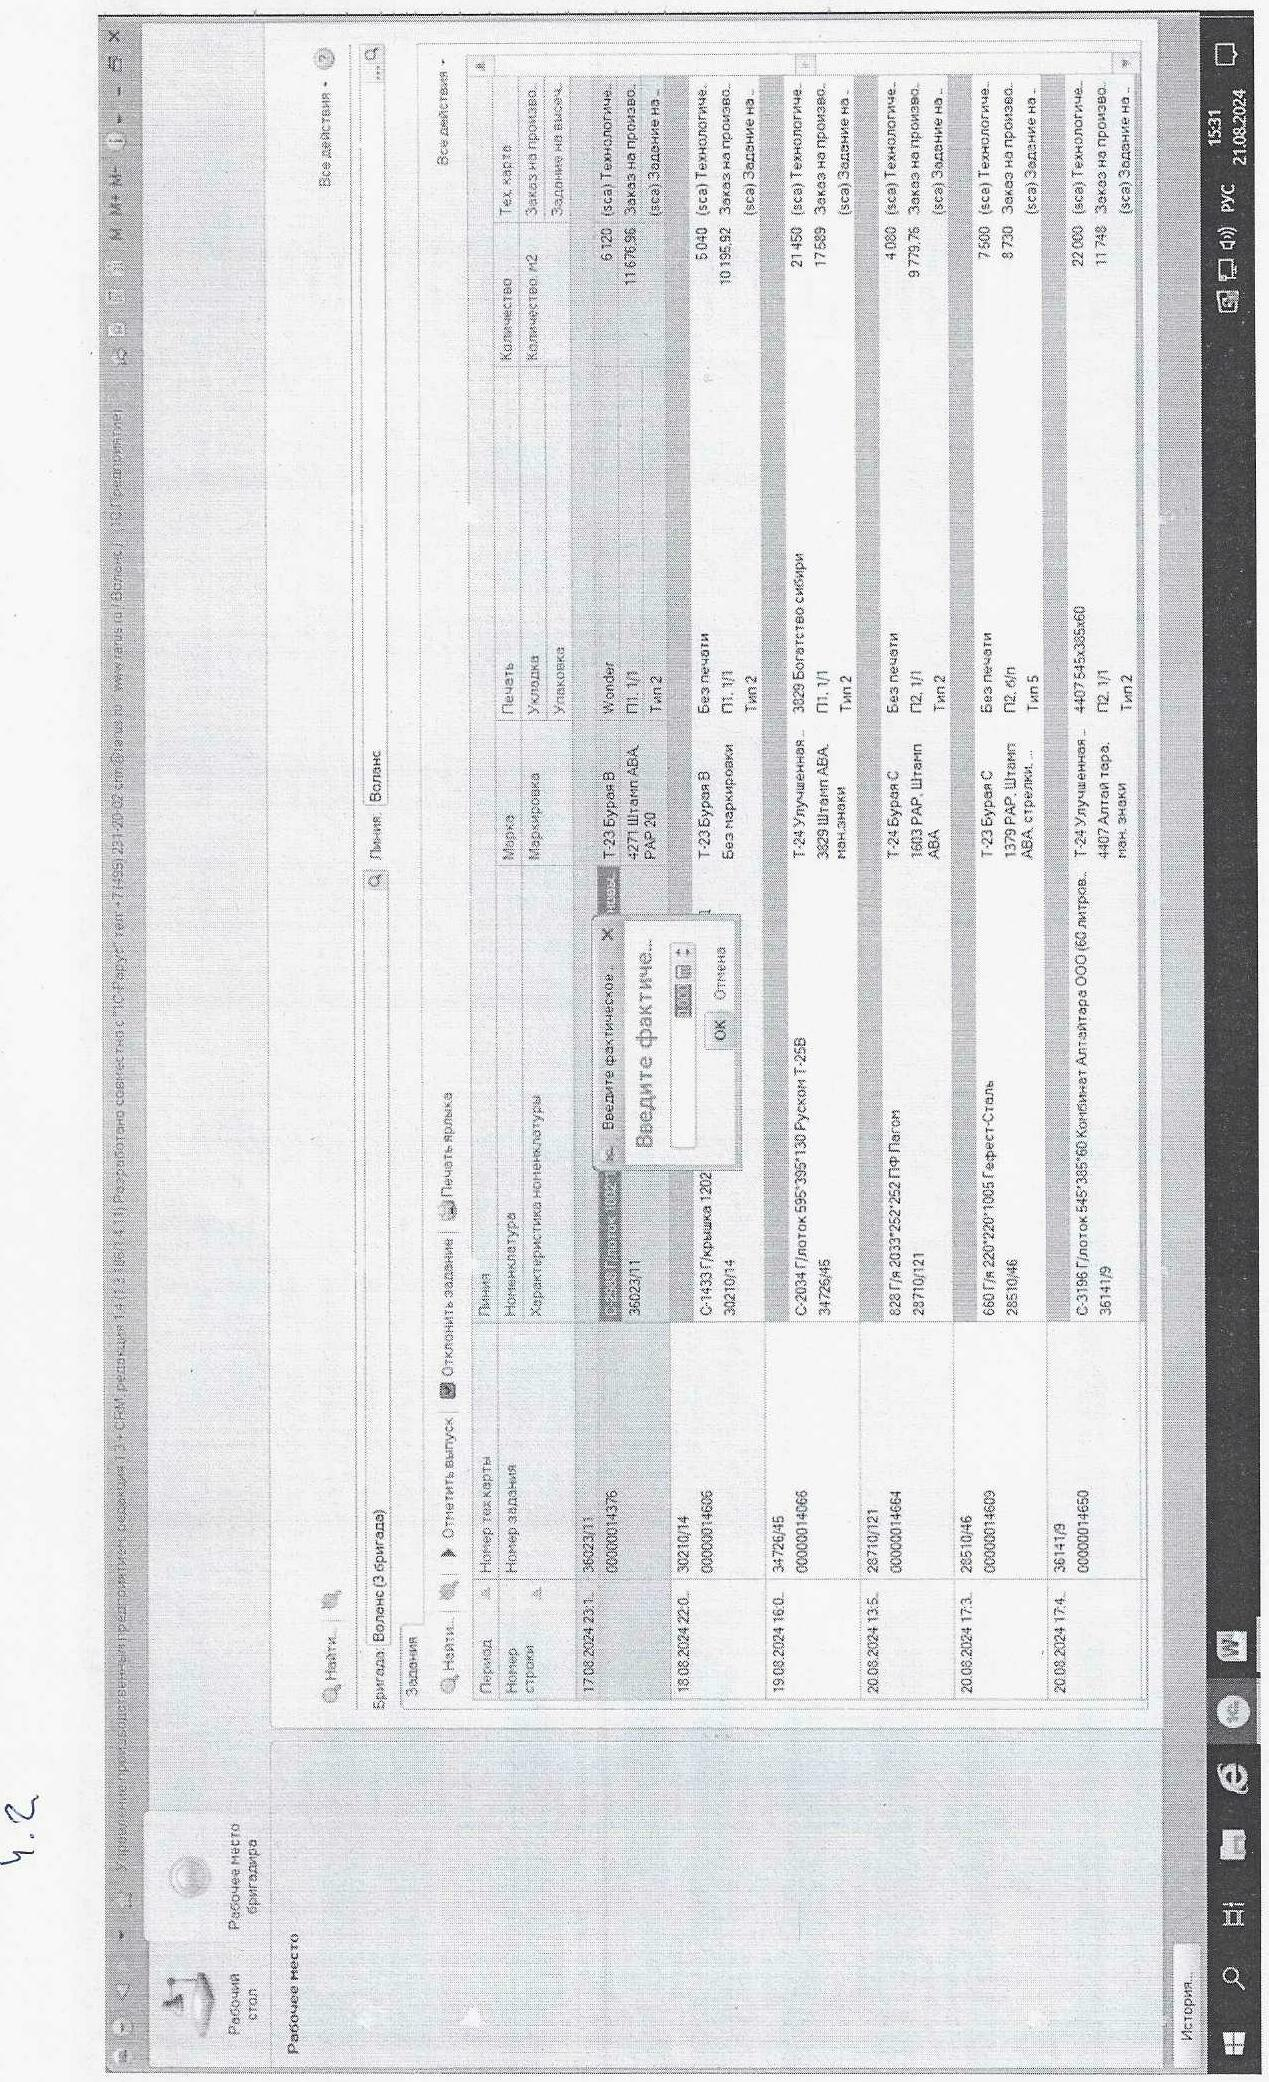
\includegraphics[height=0.94\textheight, width=0.94\textwidth, keepaspectratio]{Pics 1/4.2 рабочее место бригадира в УПП_0001.jpg}
\end{center}
  \caption{Рабочее место бригадира в 1С:УПП}
  \label{pic:4.2 рабочее место бригадира в УПП_0001}
\end{figure}

\begin{figure}
\begin{center}
  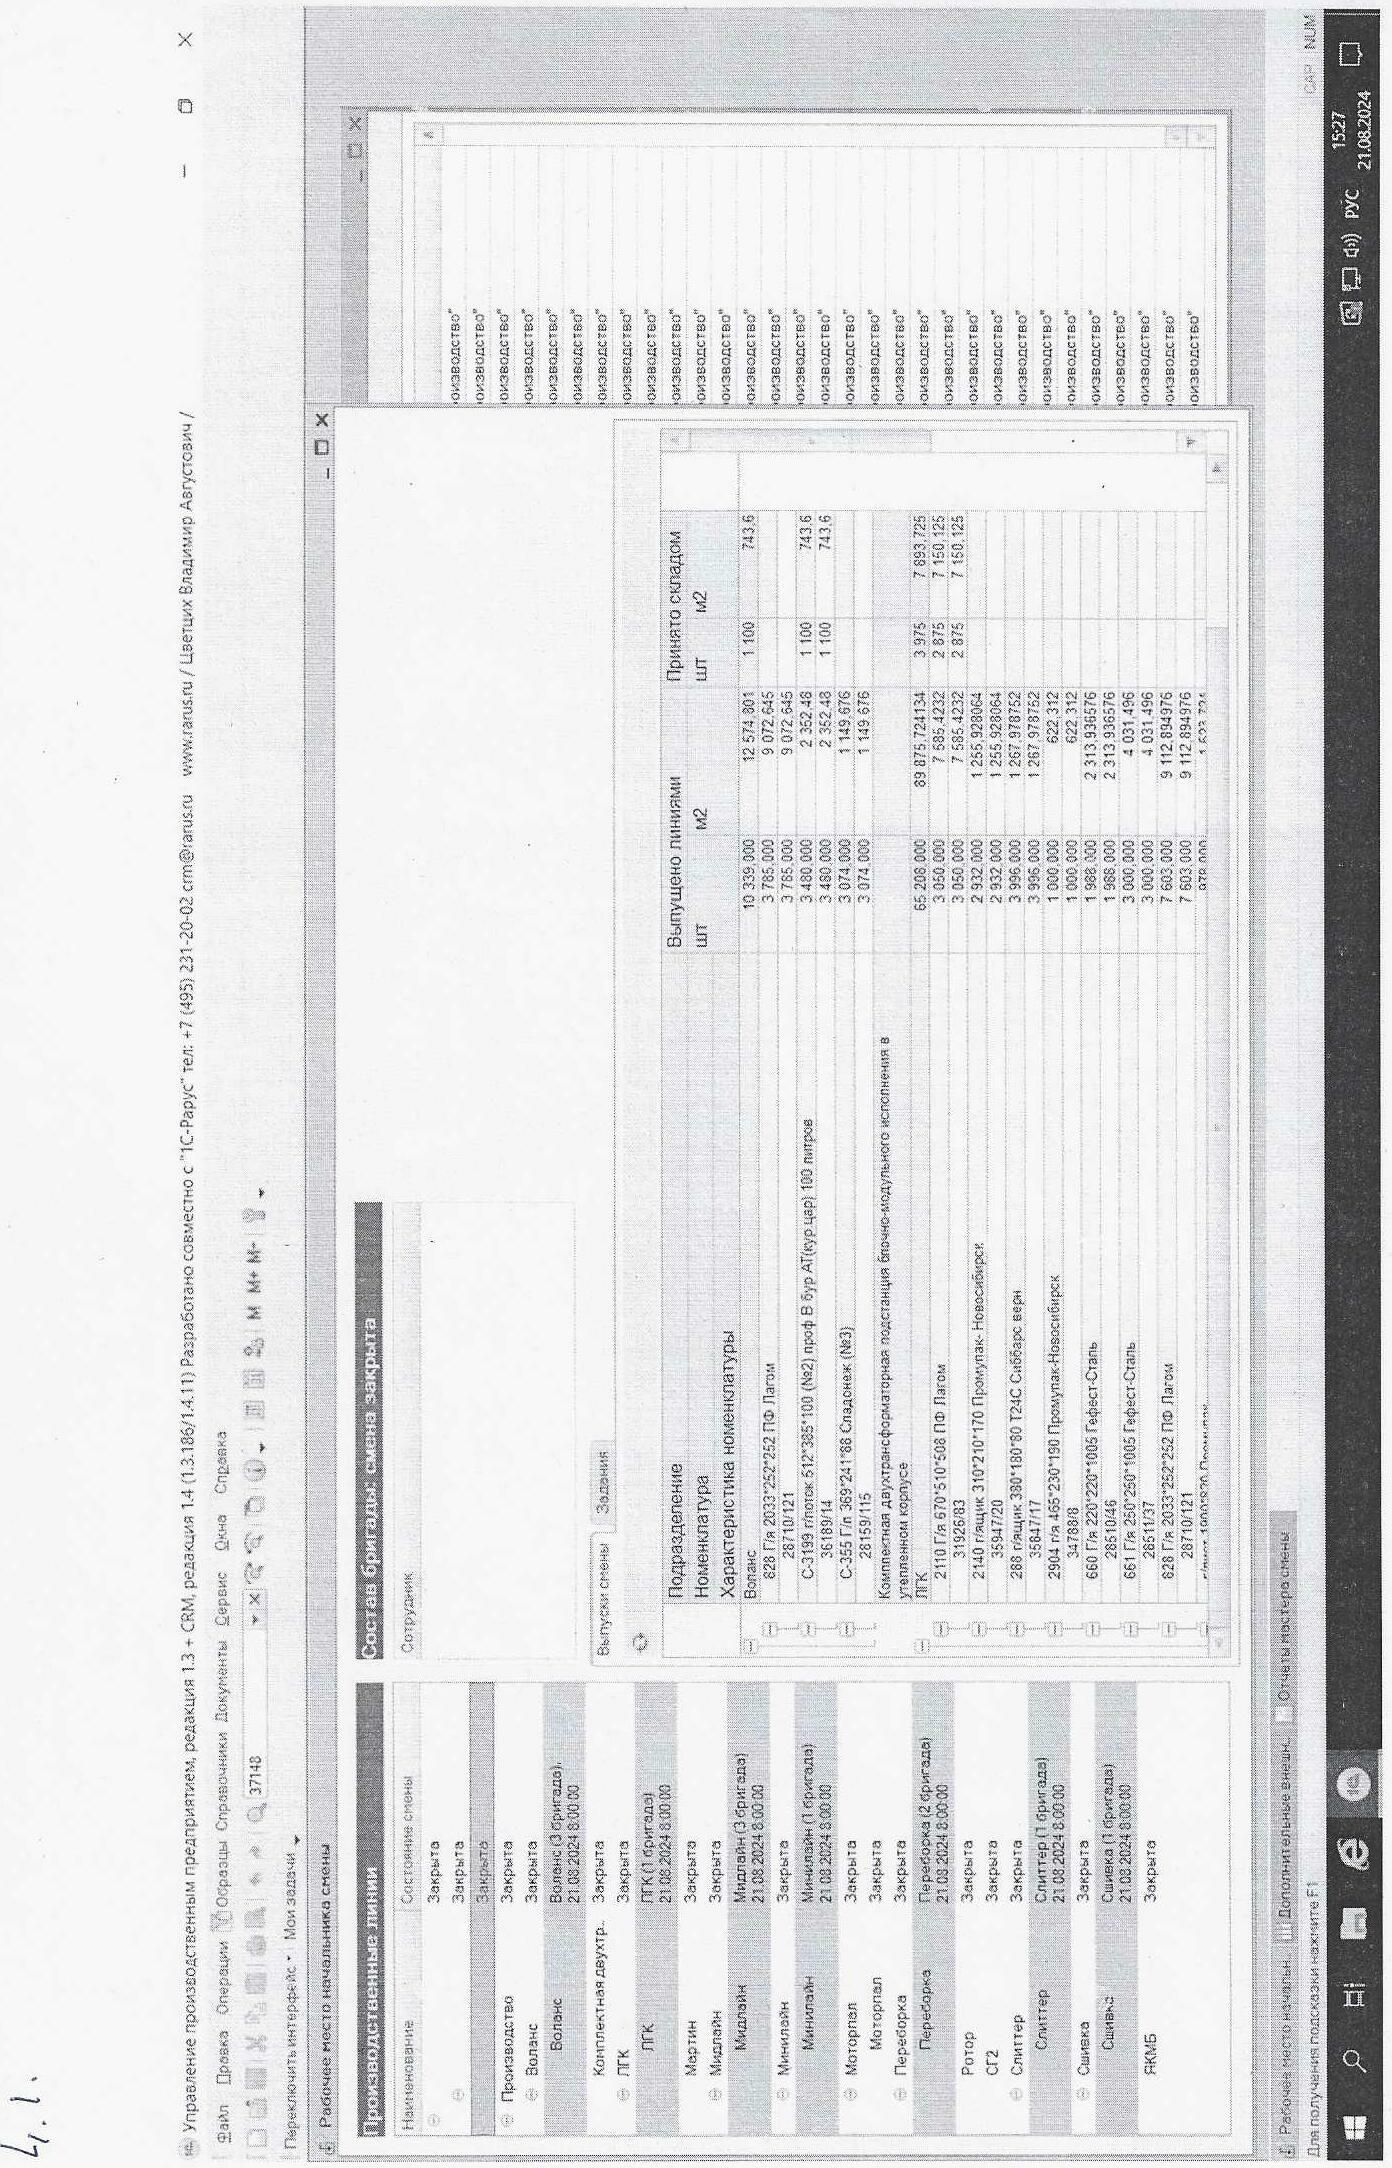
\includegraphics[height=0.94\textheight, width=0.94\textwidth, keepaspectratio]{Pics 1/4.1 рабочее место начсмены в упп_0001.jpg}
\end{center}
  \caption{Рабочее место начальника смены в 1С:УПП}
  \label{pic:4.1 рабочее место начсмены в упп_0001}
\end{figure}

\begin{figure}
\begin{center}
  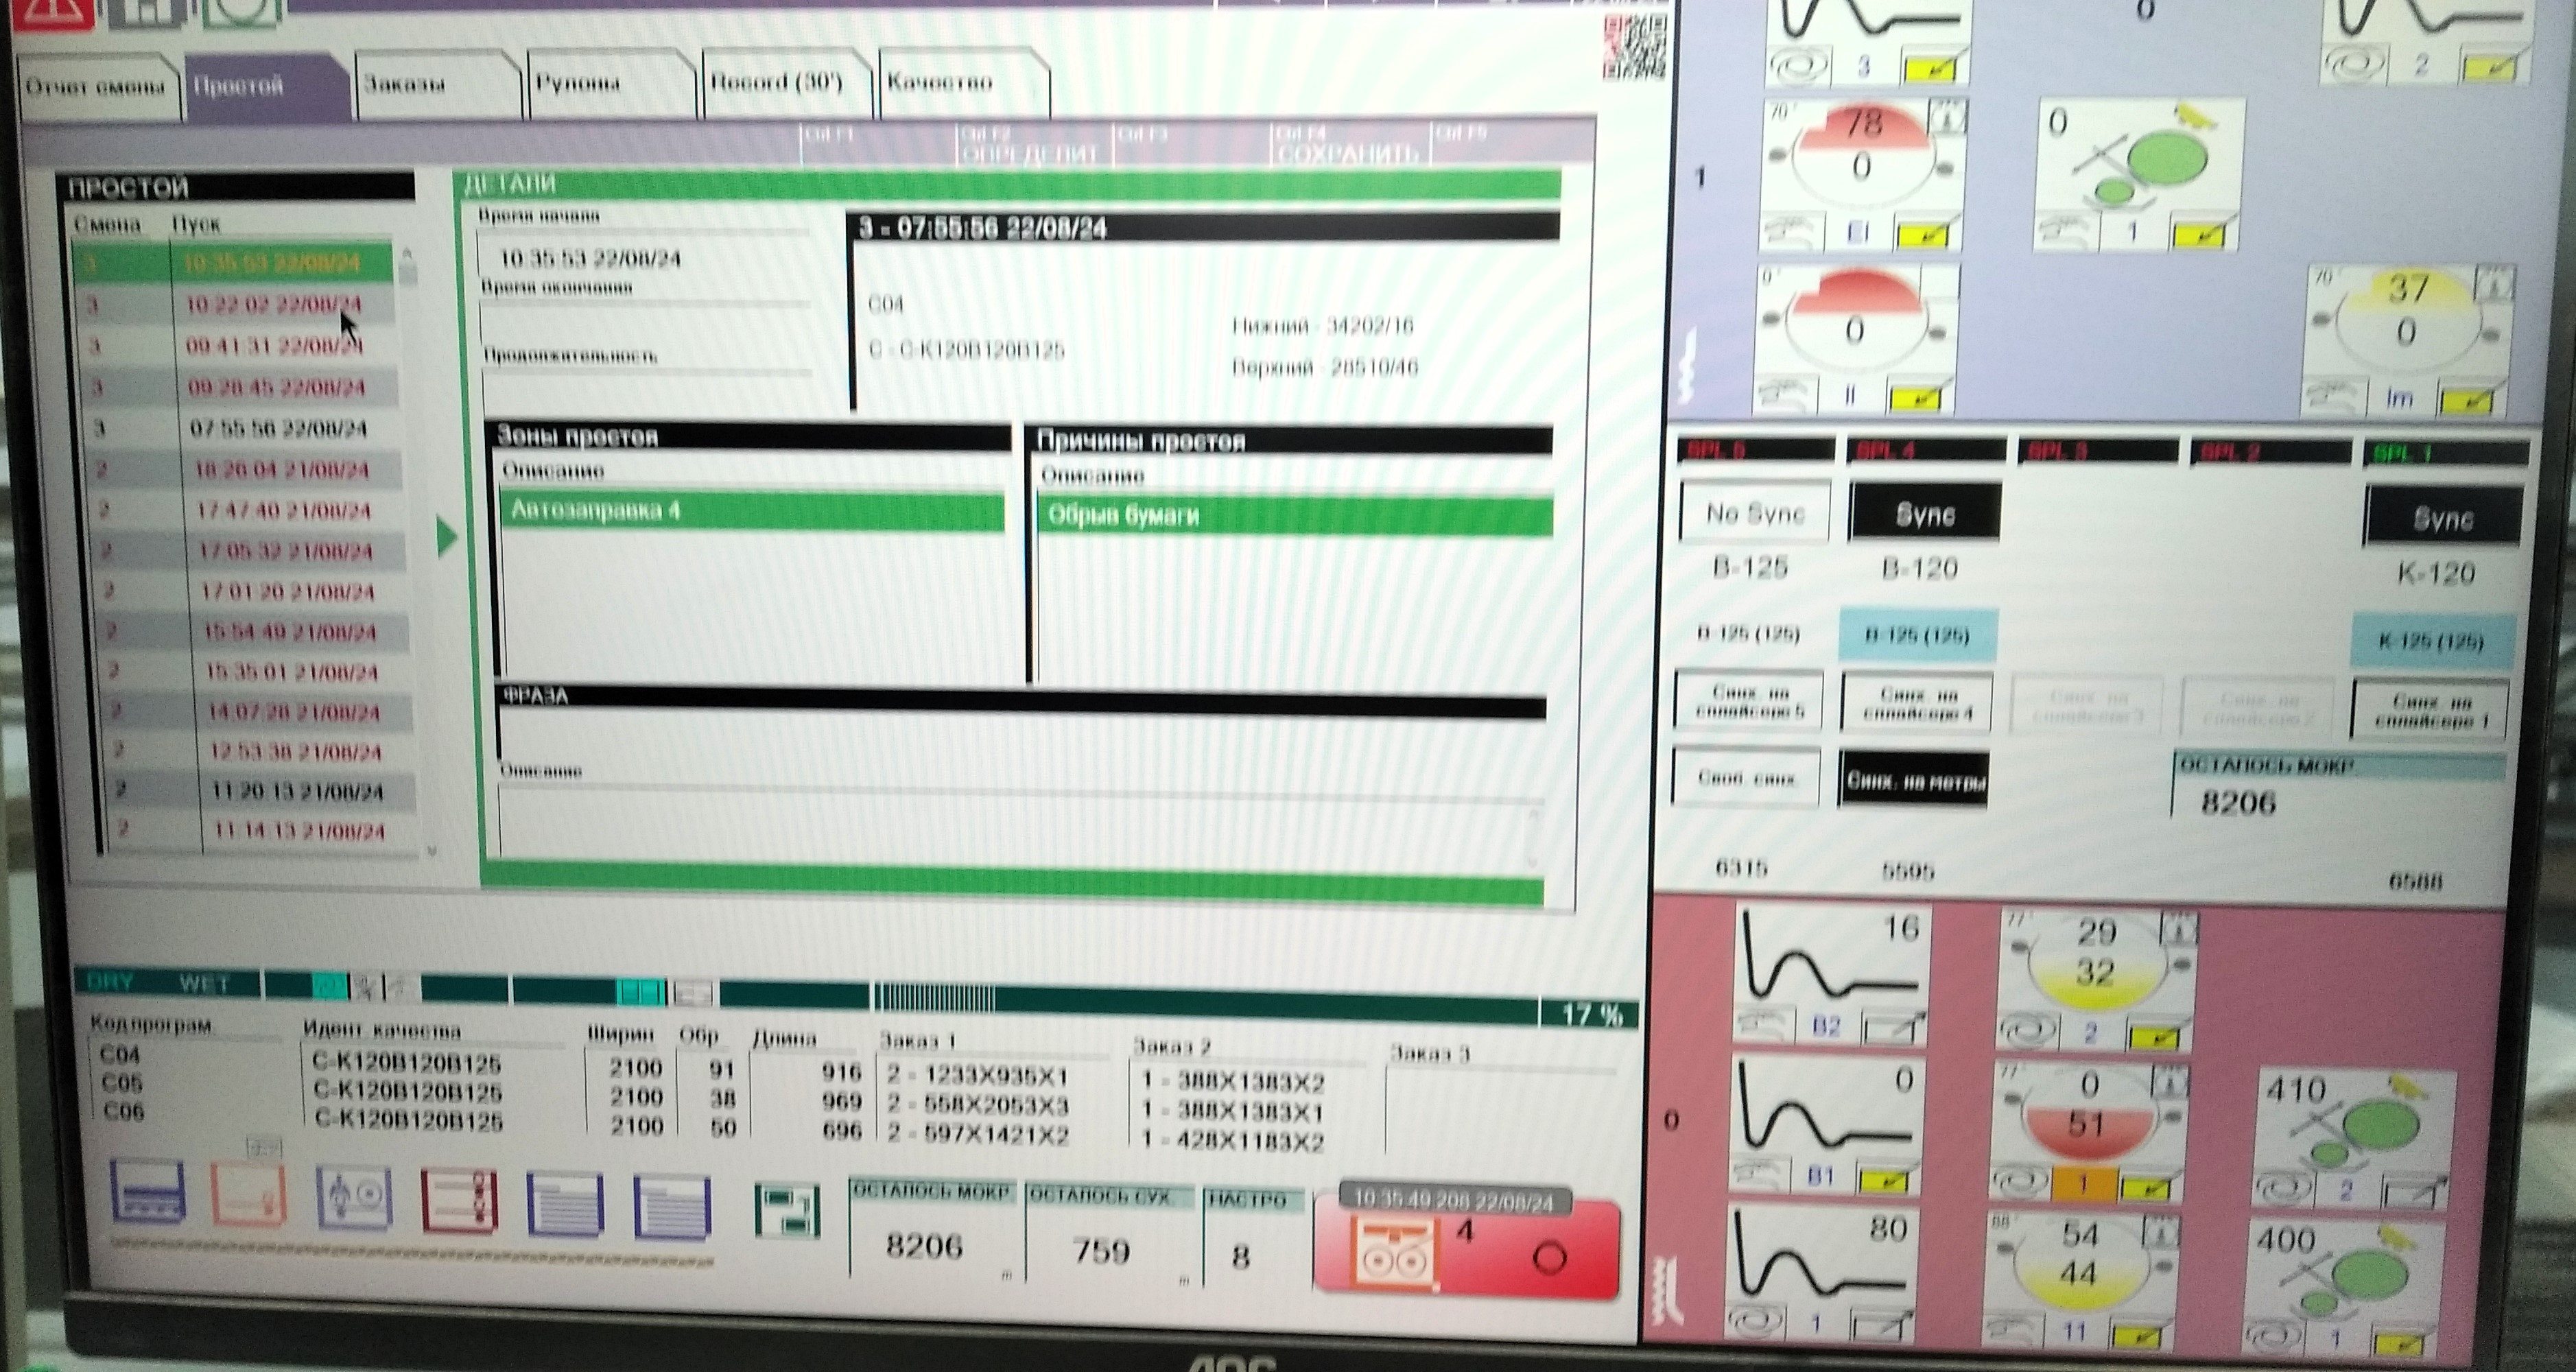
\includegraphics[height=0.94\textheight, width=0.94\textwidth, keepaspectratio]{Pics 1/5 Простои в синхро.jpg }
\end{center}
  \caption{Фиксация простоев в Syncro}
  \label{pic:5 Простои в синхро}
\end{figure}

\begin{figure}
\begin{center}
  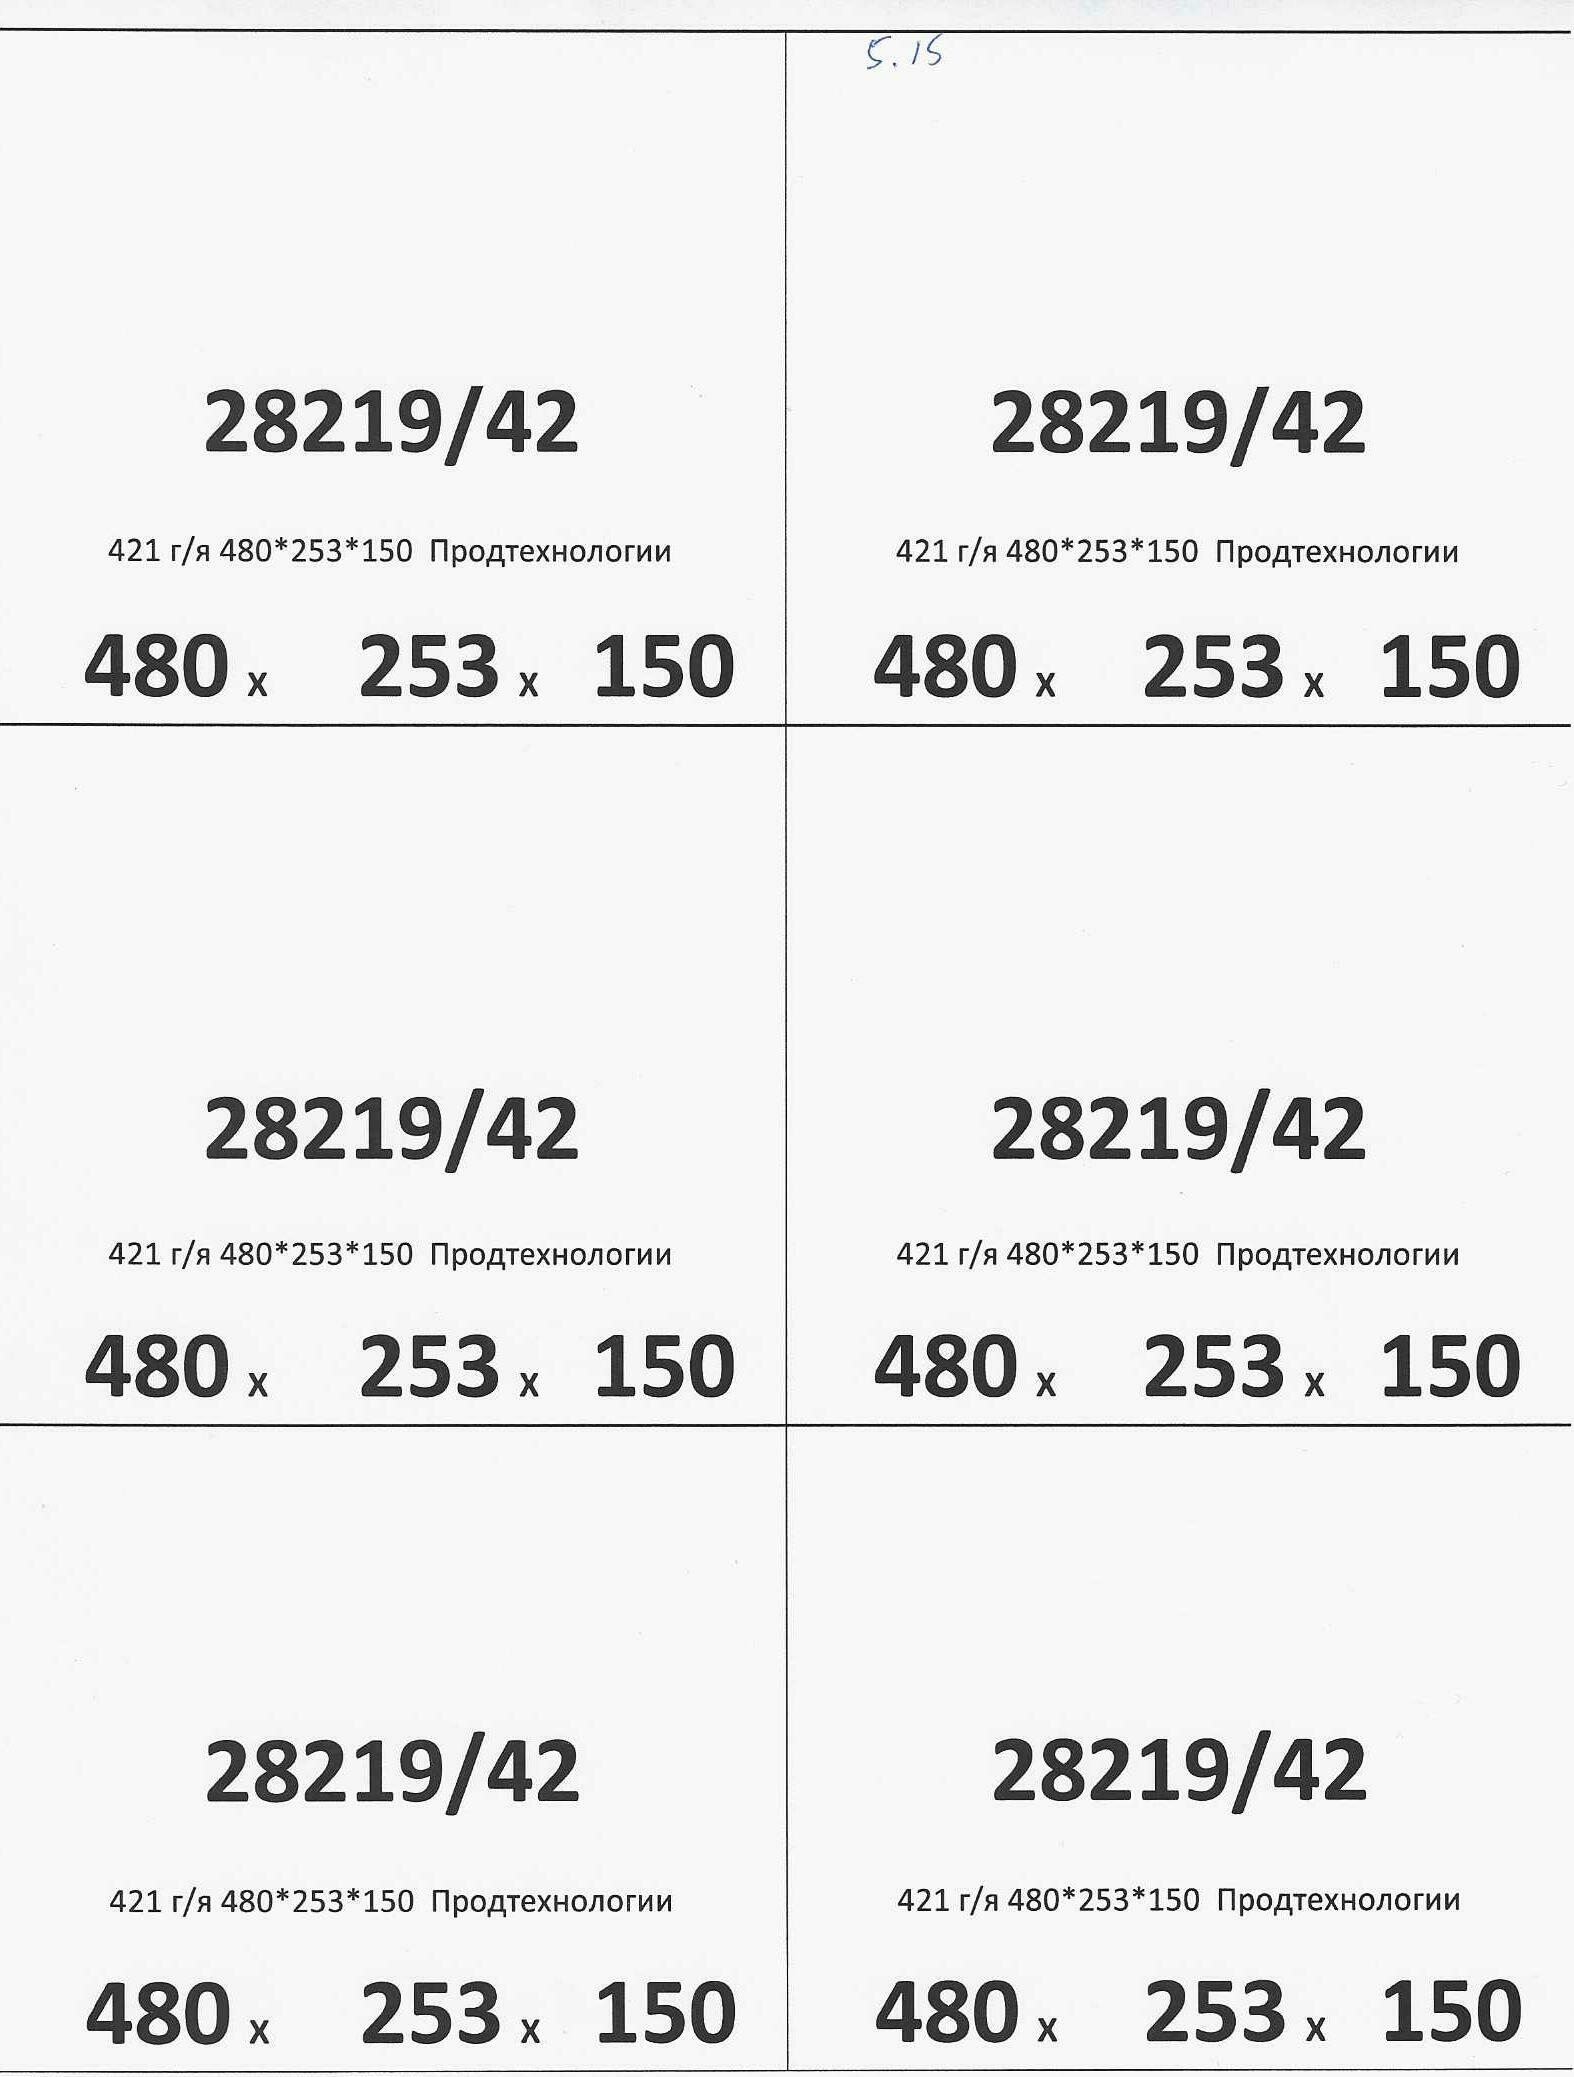
\includegraphics[height=0.94\textheight, width=0.94\textwidth, keepaspectratio]{Pics 1/5.15 ярлыки с ГА_0001.jpg}
\end{center}
  \caption{Образец ярлыка}
  \label{pic:5.15 ярлыки с ГА_0001}
\end{figure}

\begin{figure}
\begin{center}
  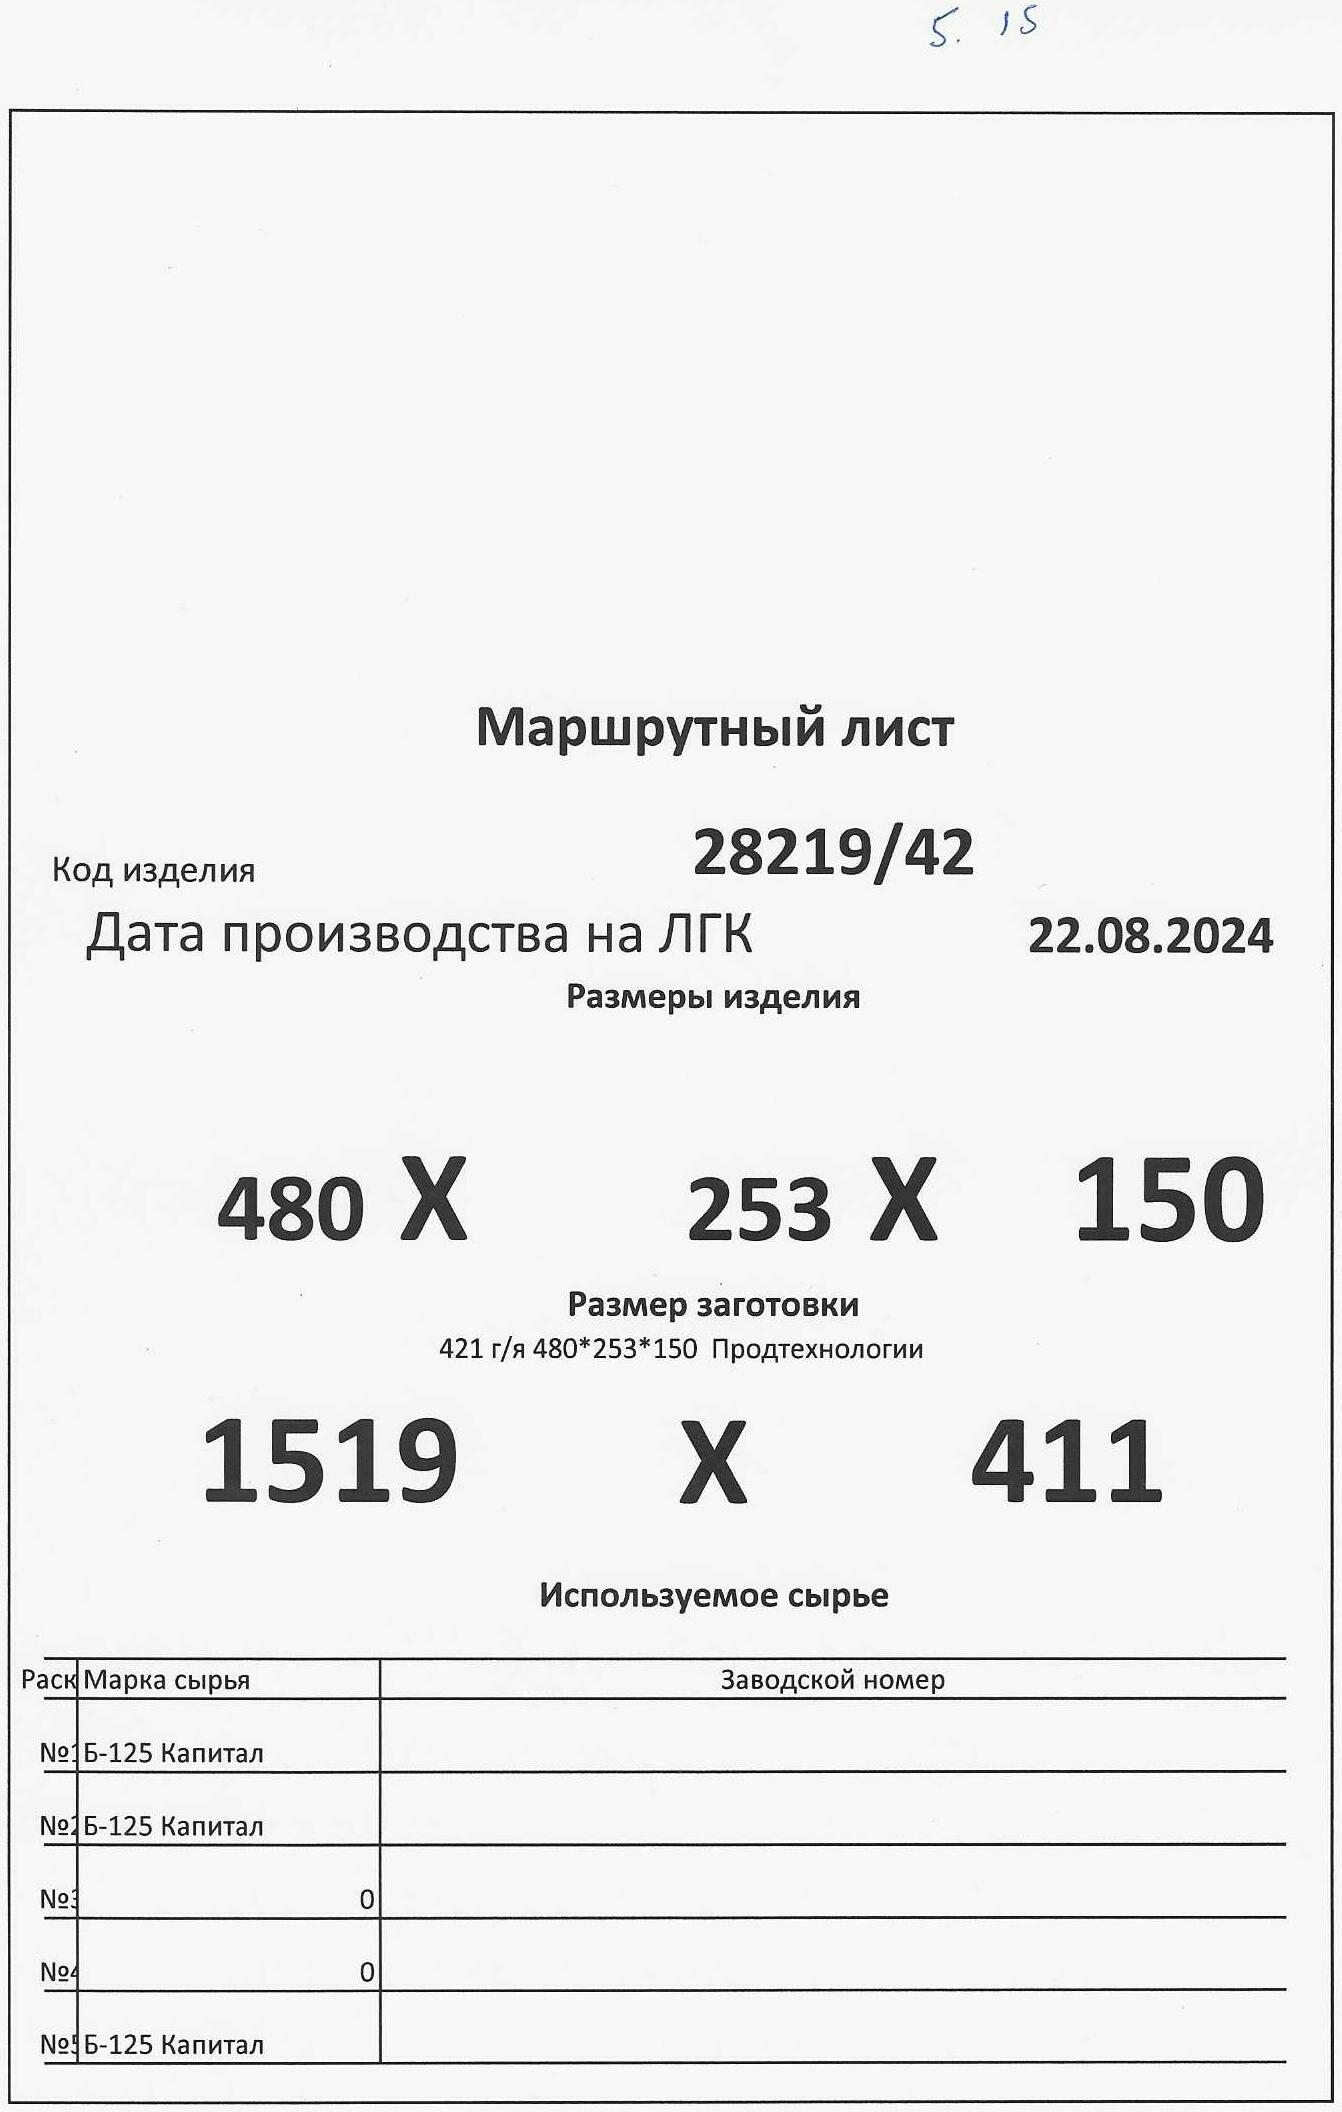
\includegraphics[height=0.94\textheight, width=0.94\textwidth, keepaspectratio]{Pics 1/5.15 маршрутный лист с ГА_0001.jpg}
\end{center}
  \caption{Образец маршрутного листа}
  \label{pic:5.15 маршрутный лист с ГА_0001}
\end{figure}

\begin{figure}
\begin{center}
  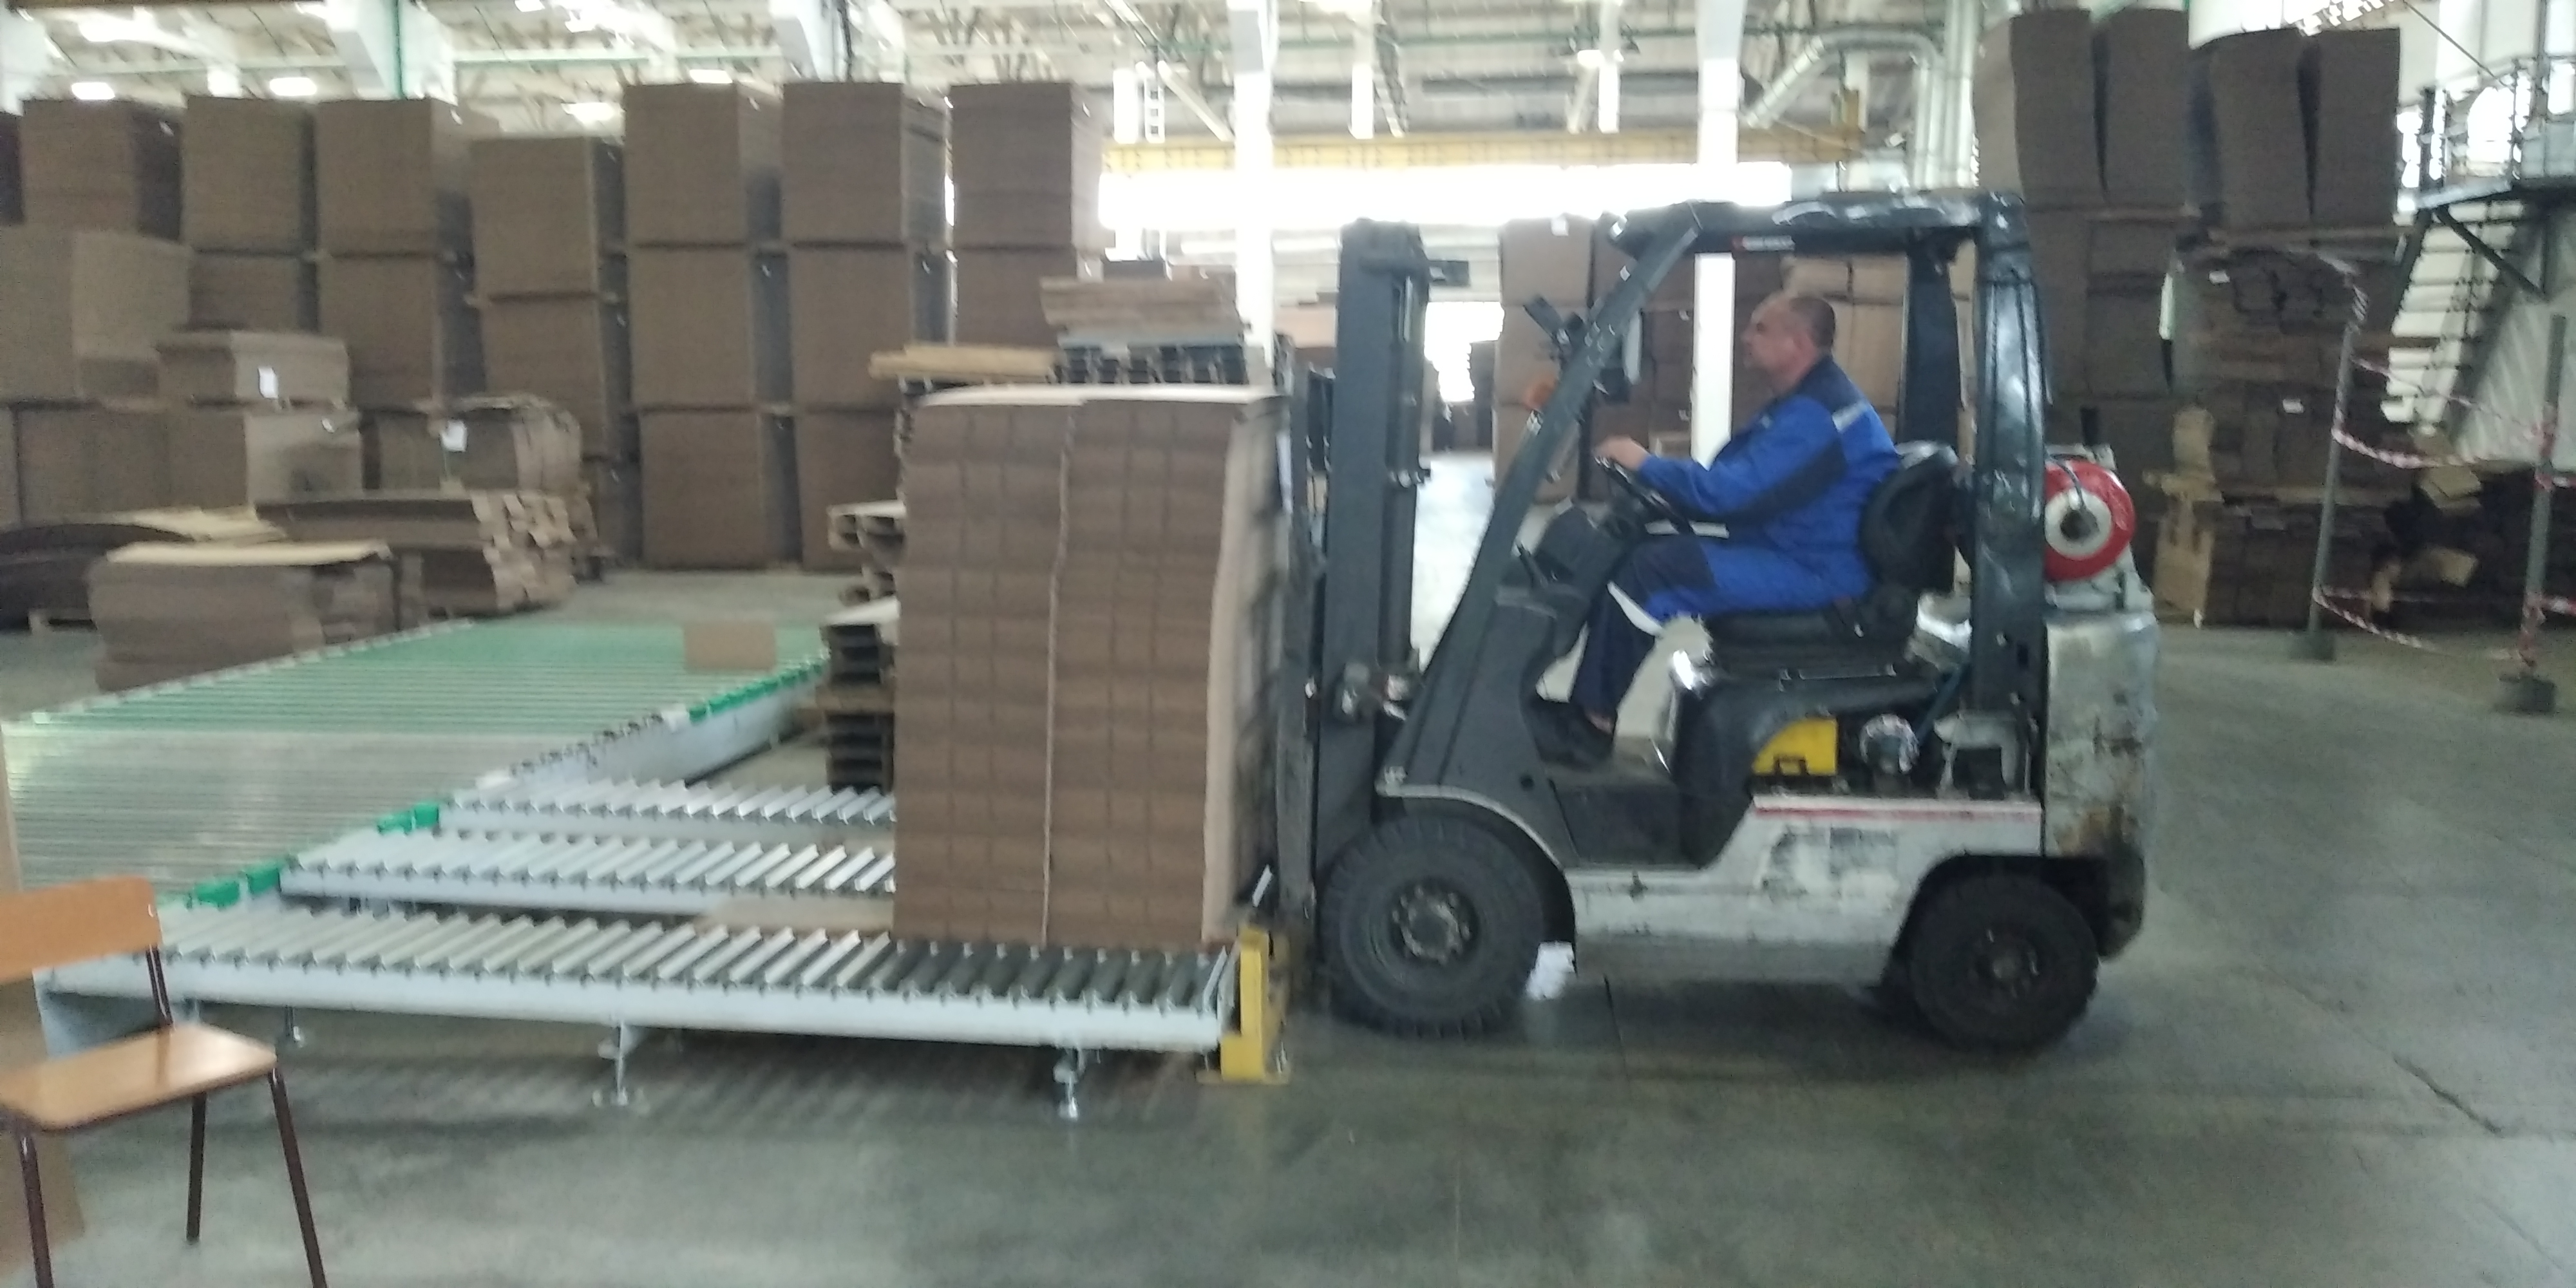
\includegraphics[height=0.94\textheight, width=0.94\textwidth, keepaspectratio]{Pics 1/5 Съем заготовок с ГА.jpg}
\end{center}
  \caption{Перемещение заготовок}
  \label{pic:5 Съем заготовок с ГА}
\end{figure}

\begin{figure}
\begin{center}
  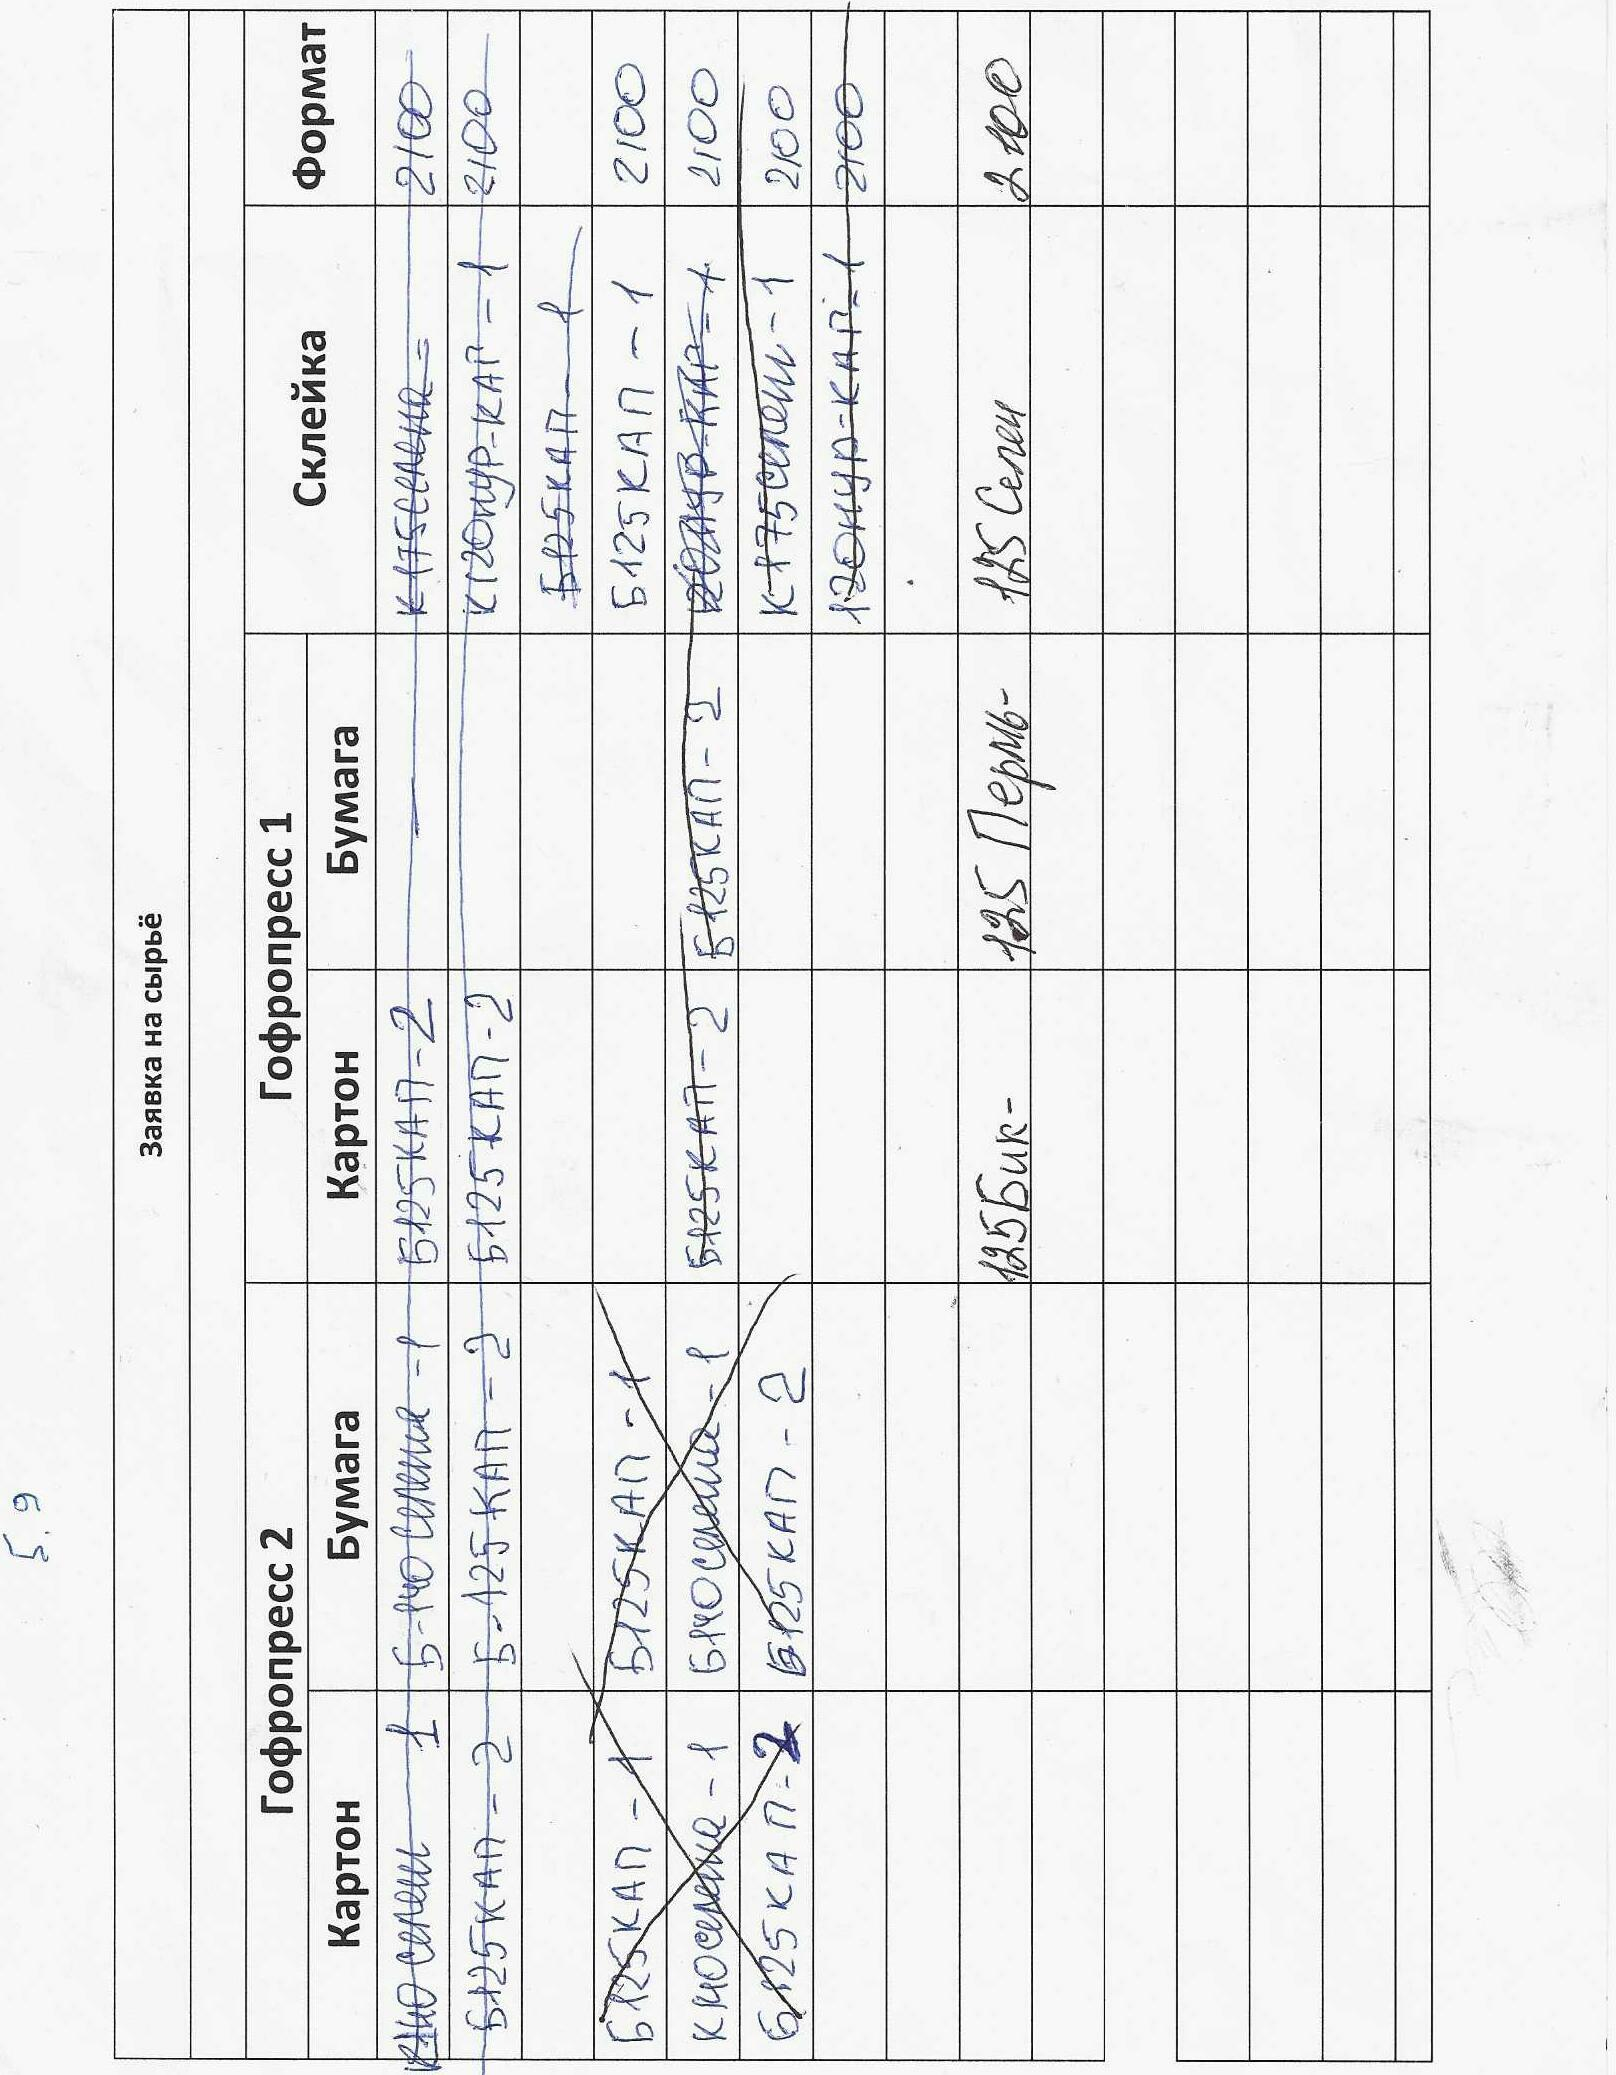
\includegraphics[height=0.94\textheight, width=0.94\textwidth, keepaspectratio]{Pics 1/5.9 заявка на сырье с ГА НА СКЛАД_0001.jpg }
\end{center}
  \caption{Заявка на сырье}
  \label{pic:5.9 заявка на сырье с ГА НА СКЛАД_0001}
\end{figure}

\begin{figure}
\begin{center}
  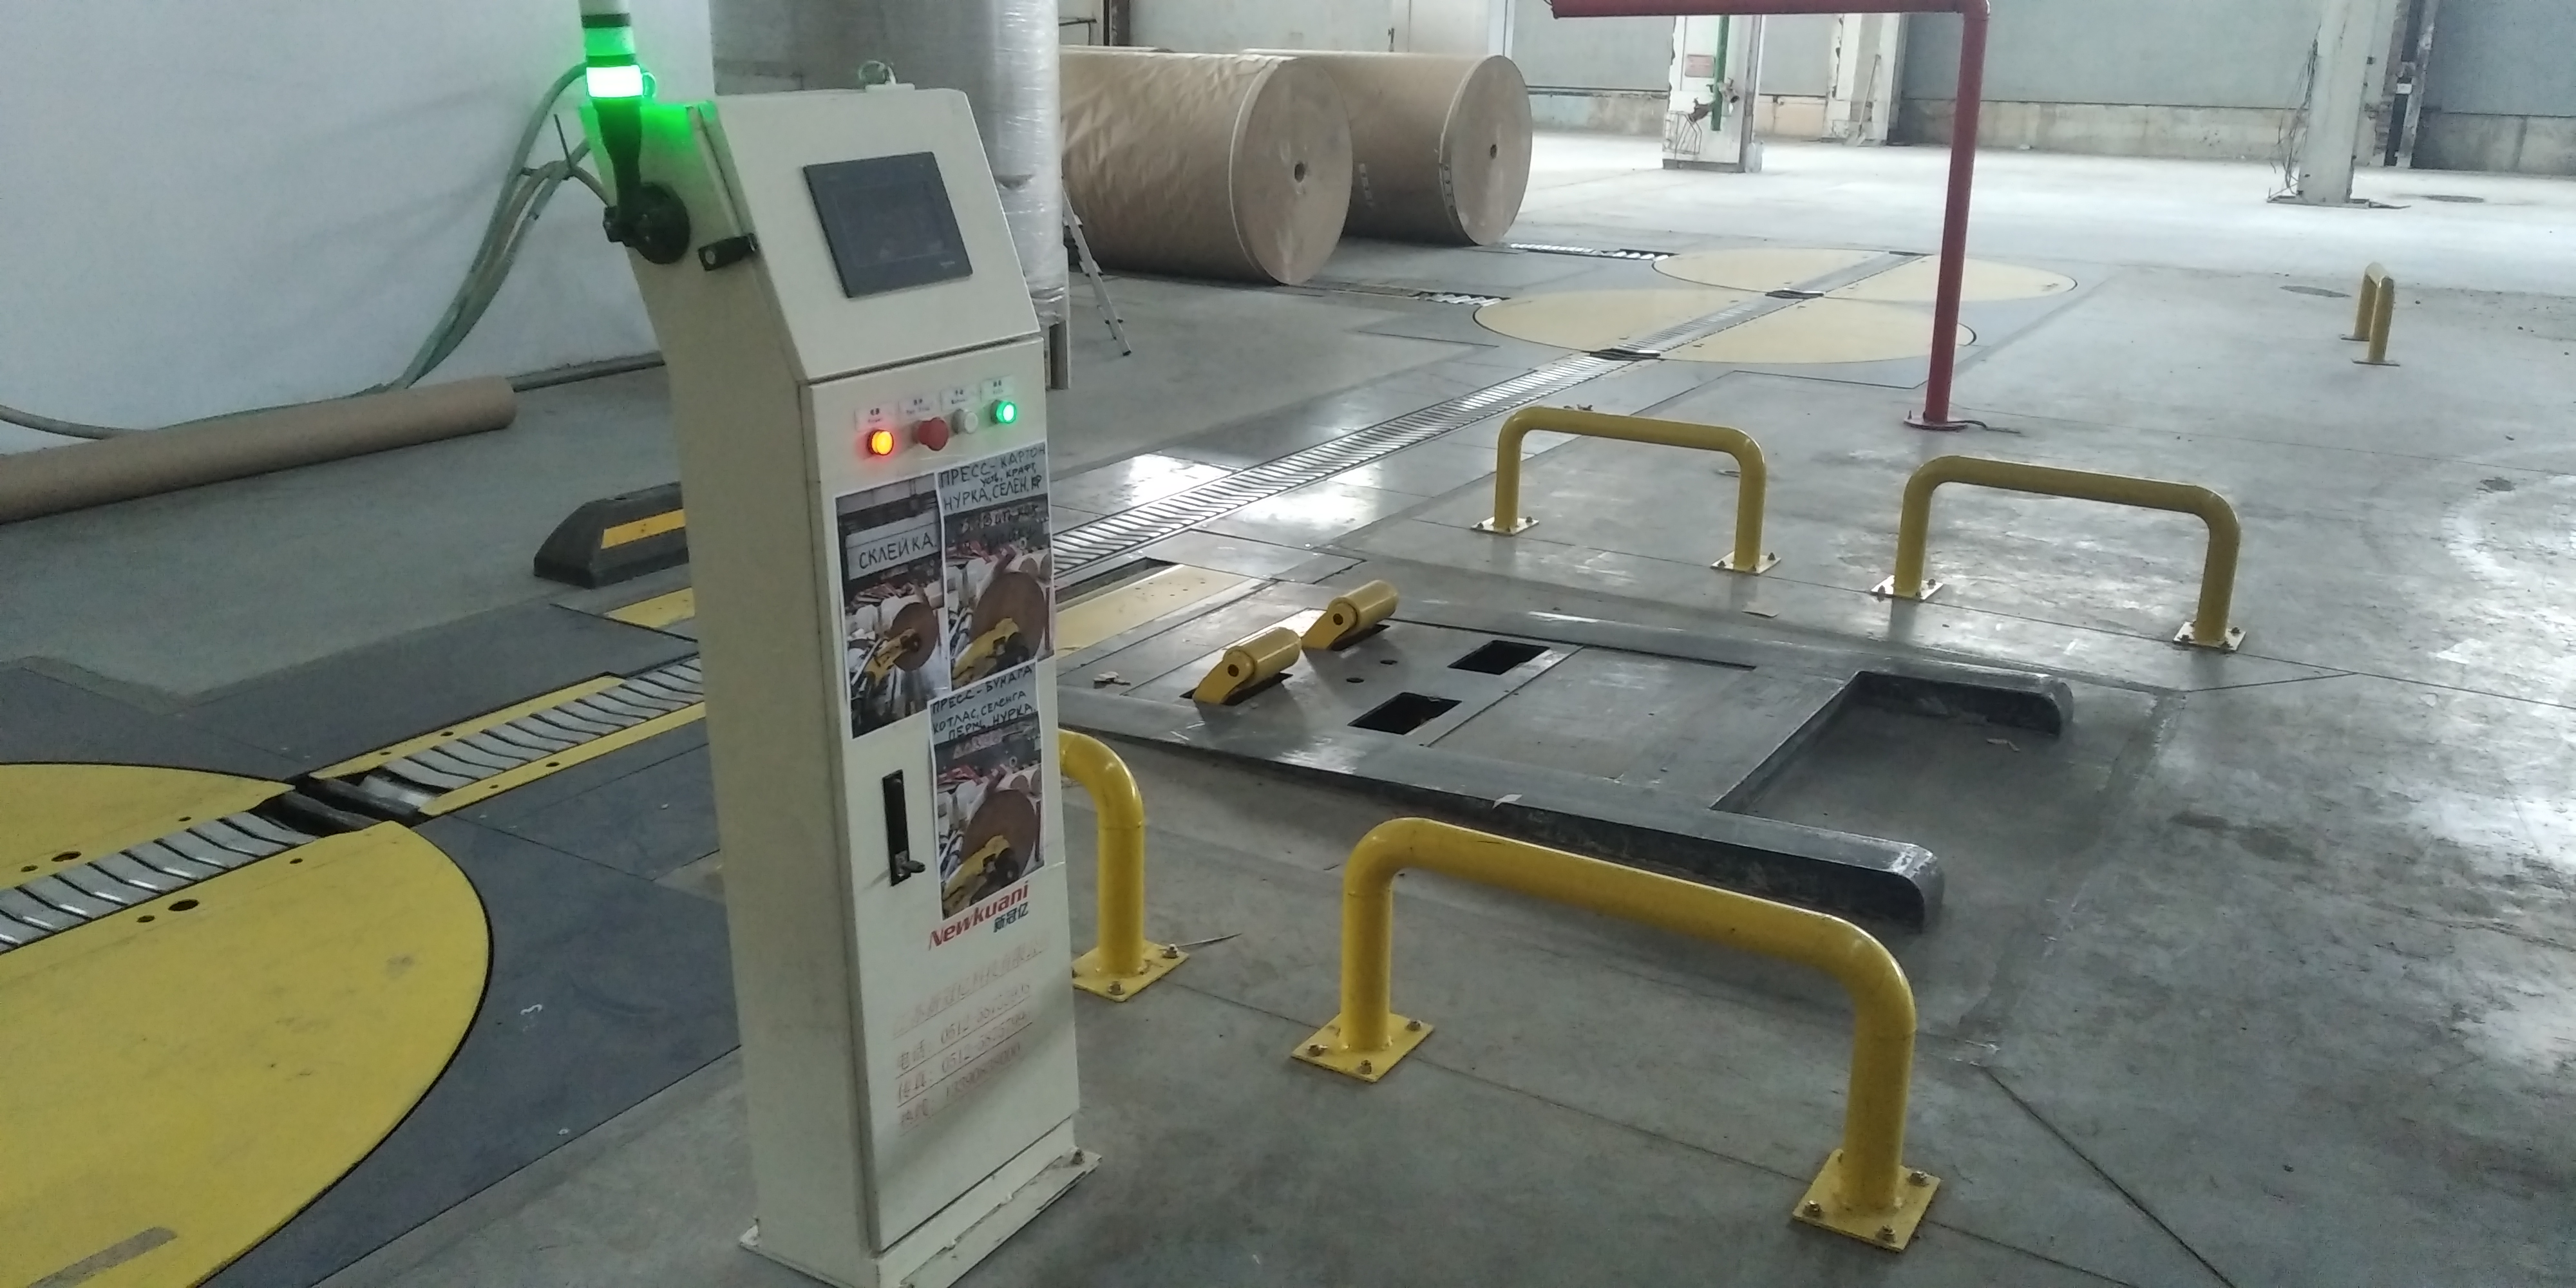
\includegraphics[height=0.94\textheight, width=0.94\textwidth, keepaspectratio]{Pics 1/5 Подача рулонов на раскаты ГА.jpg }
\end{center}
  \caption{Линия подачи рулонов}
  \label{pic:5 Подача рулонов на раскаты ГА}
\end{figure}

\begin{figure}
\begin{center}
  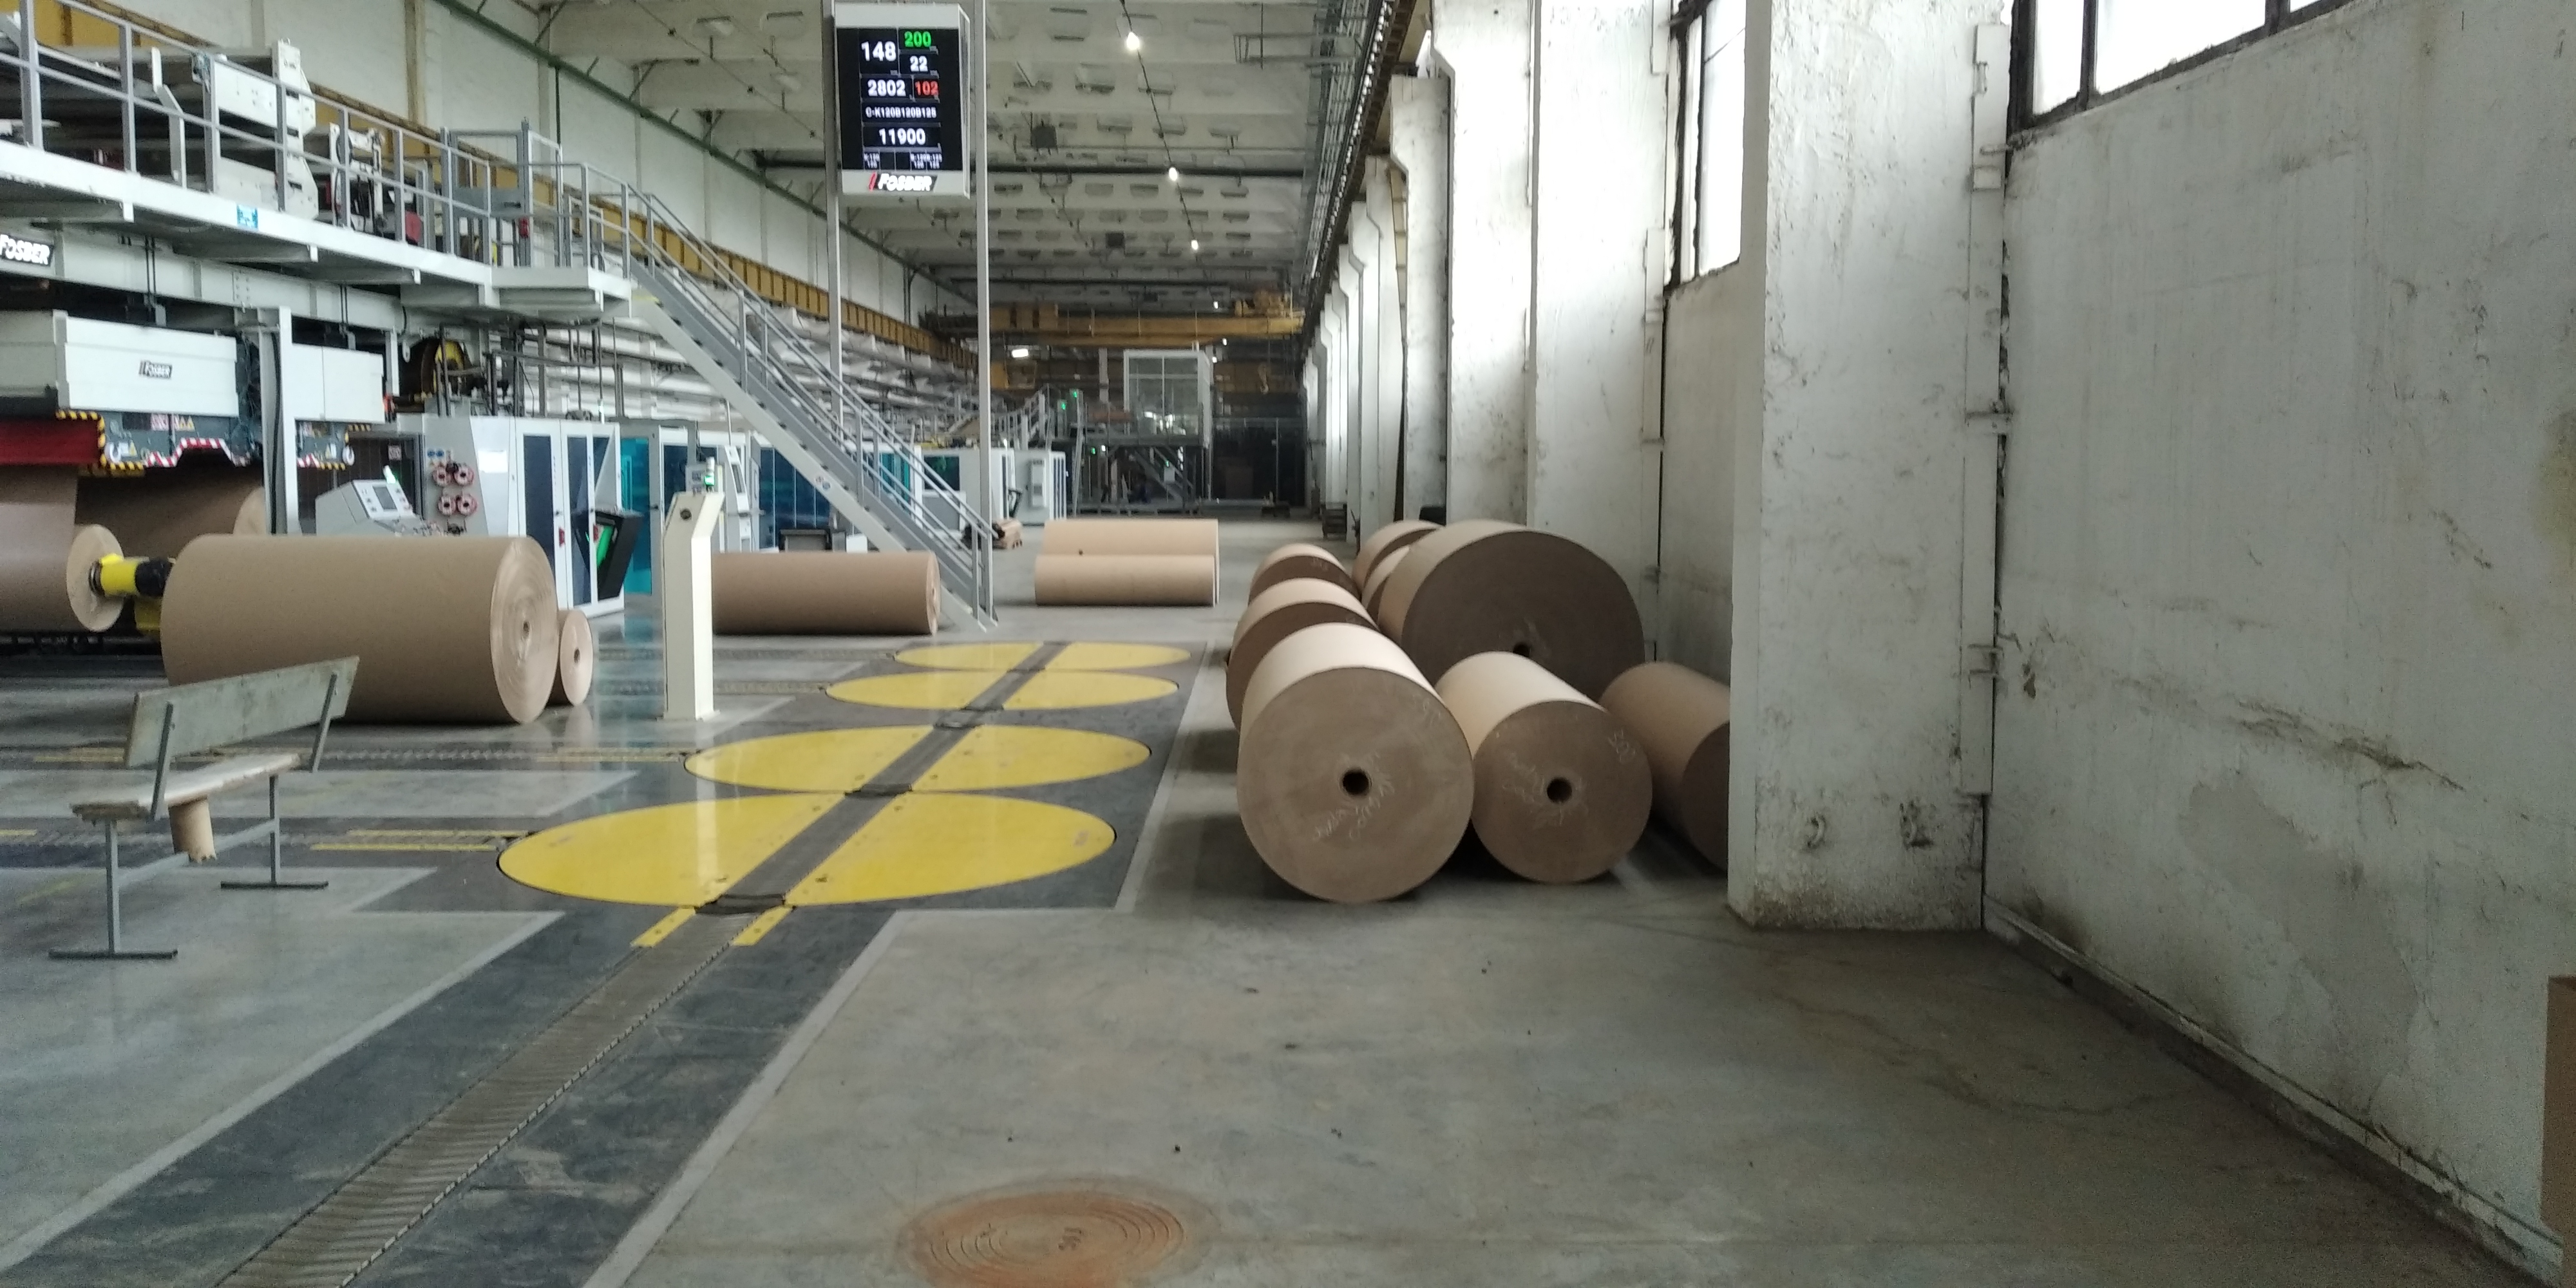
\includegraphics[height=0.94\textheight, width=0.94\textwidth, keepaspectratio]{Pics 1/5 недомоты у ГА.jpg }
\end{center}
  \caption{Недомоты}
  \label{pic:5 недомоты у ГА}
\end{figure}

\begin{figure}
\begin{center}
  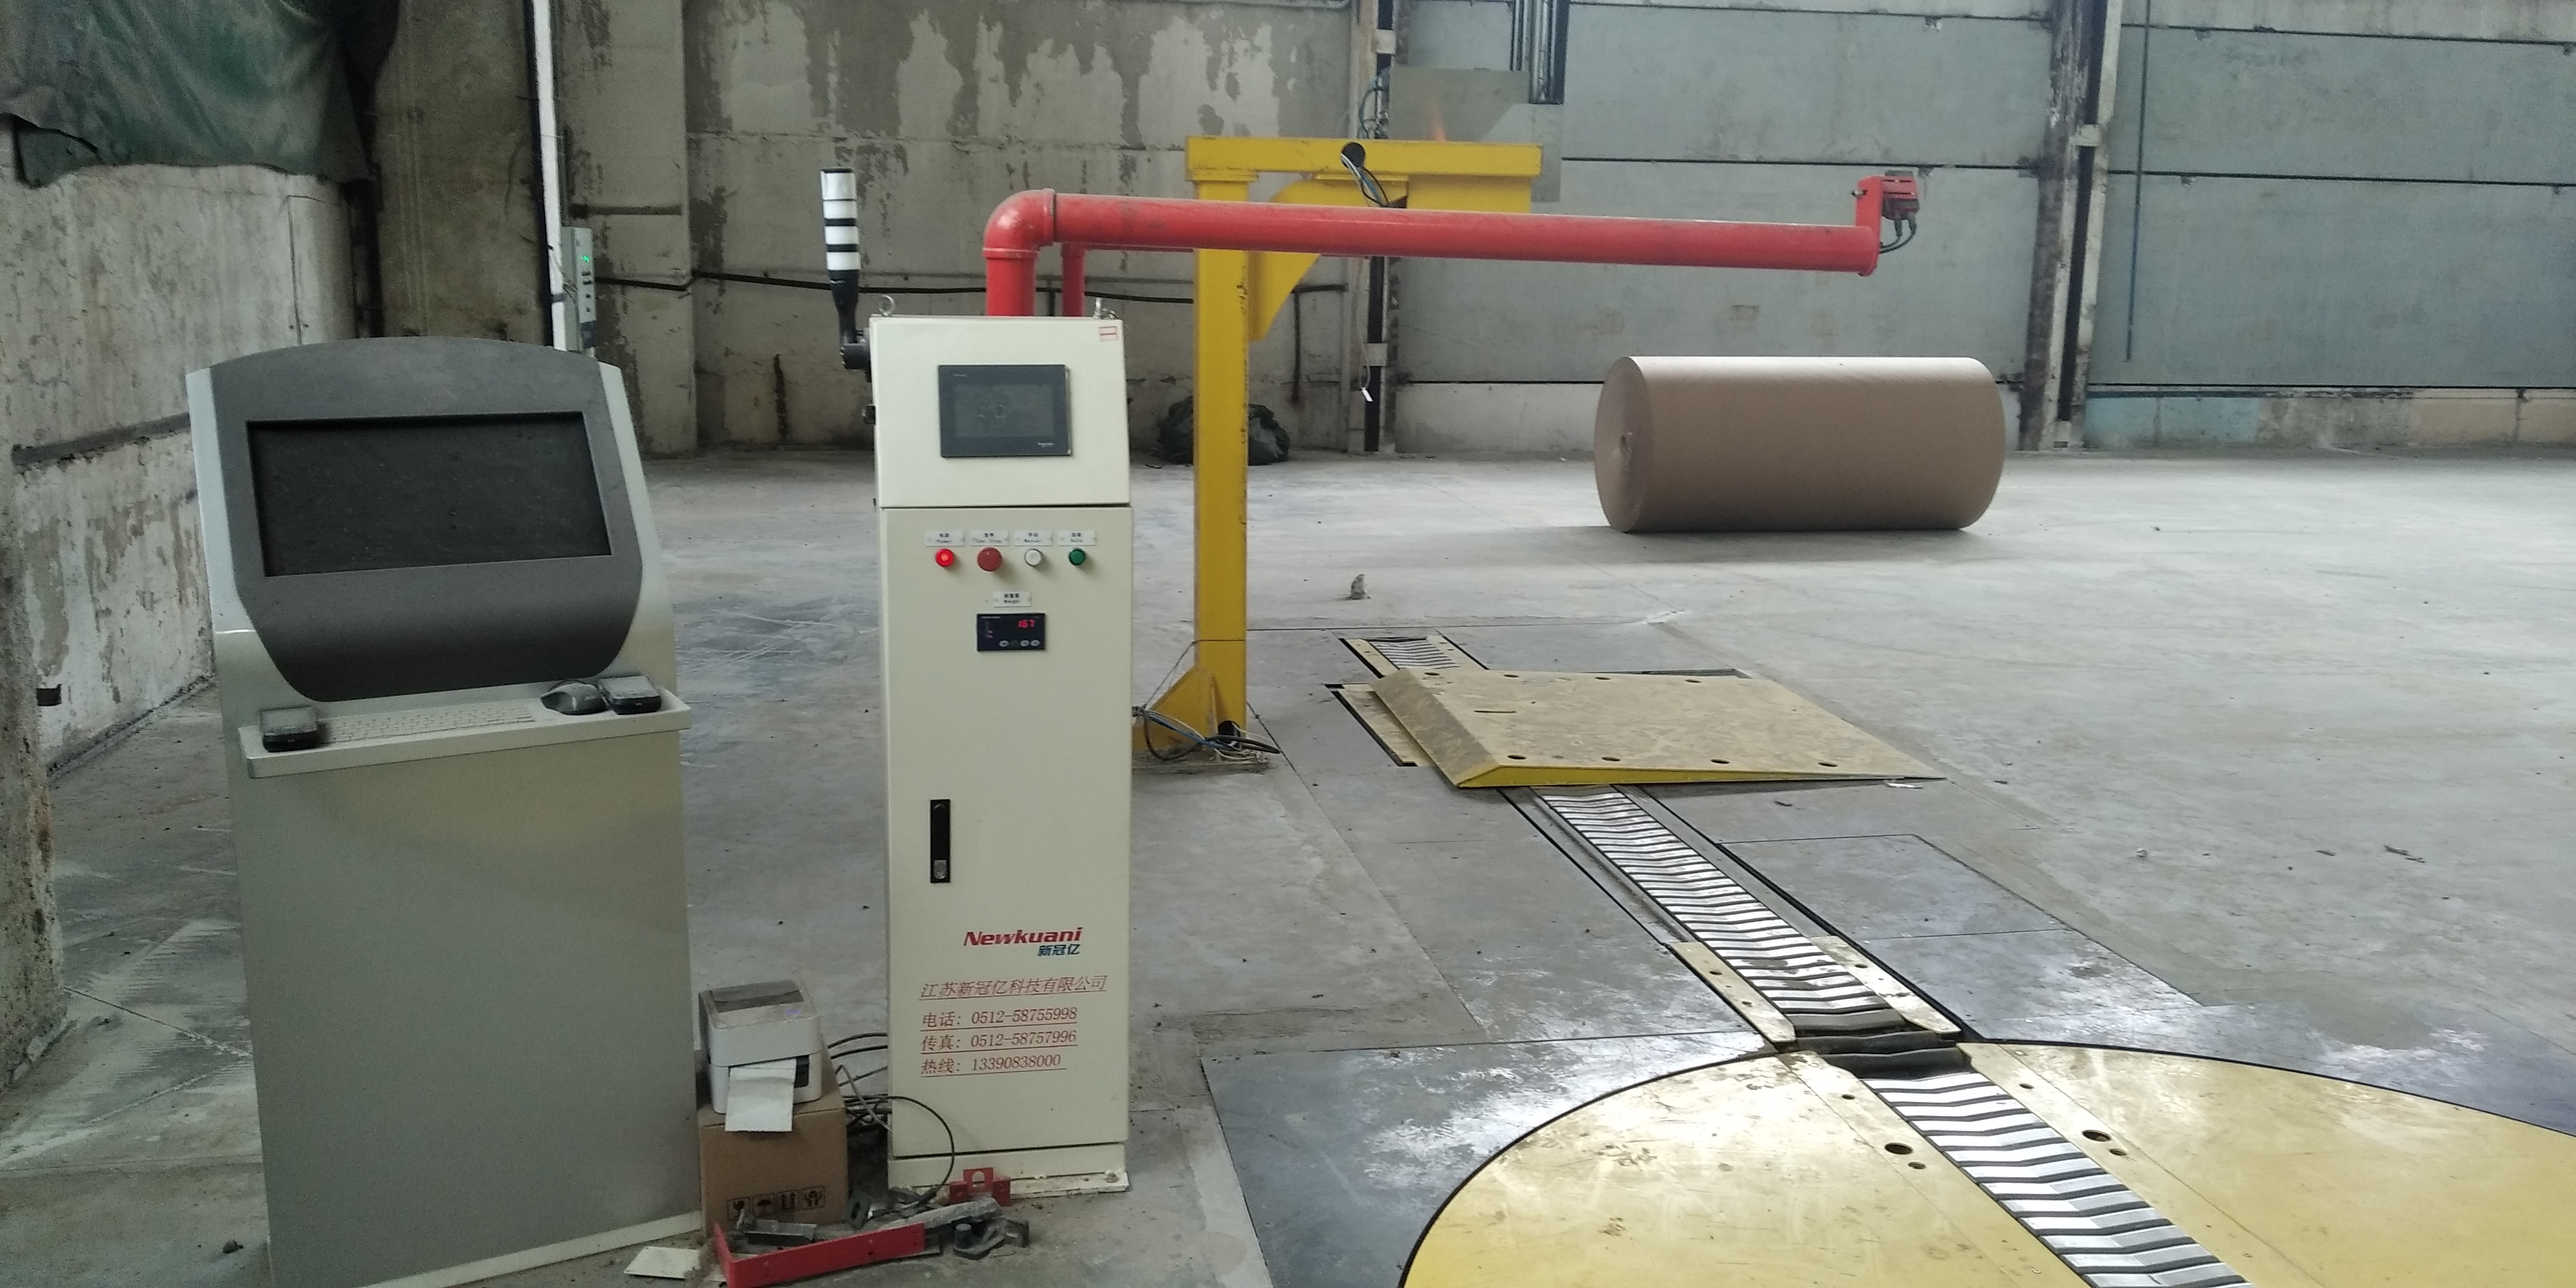
\includegraphics[height=0.94\textheight, width=0.94\textwidth, keepaspectratio]{Pics 1/5 Весы на ГА.jpg}
\end{center}
  \caption{Весы системы транспортировки рулонов}
  \label{pic:5 Весы на ГА}
\end{figure}

\begin{figure}
\begin{center}
  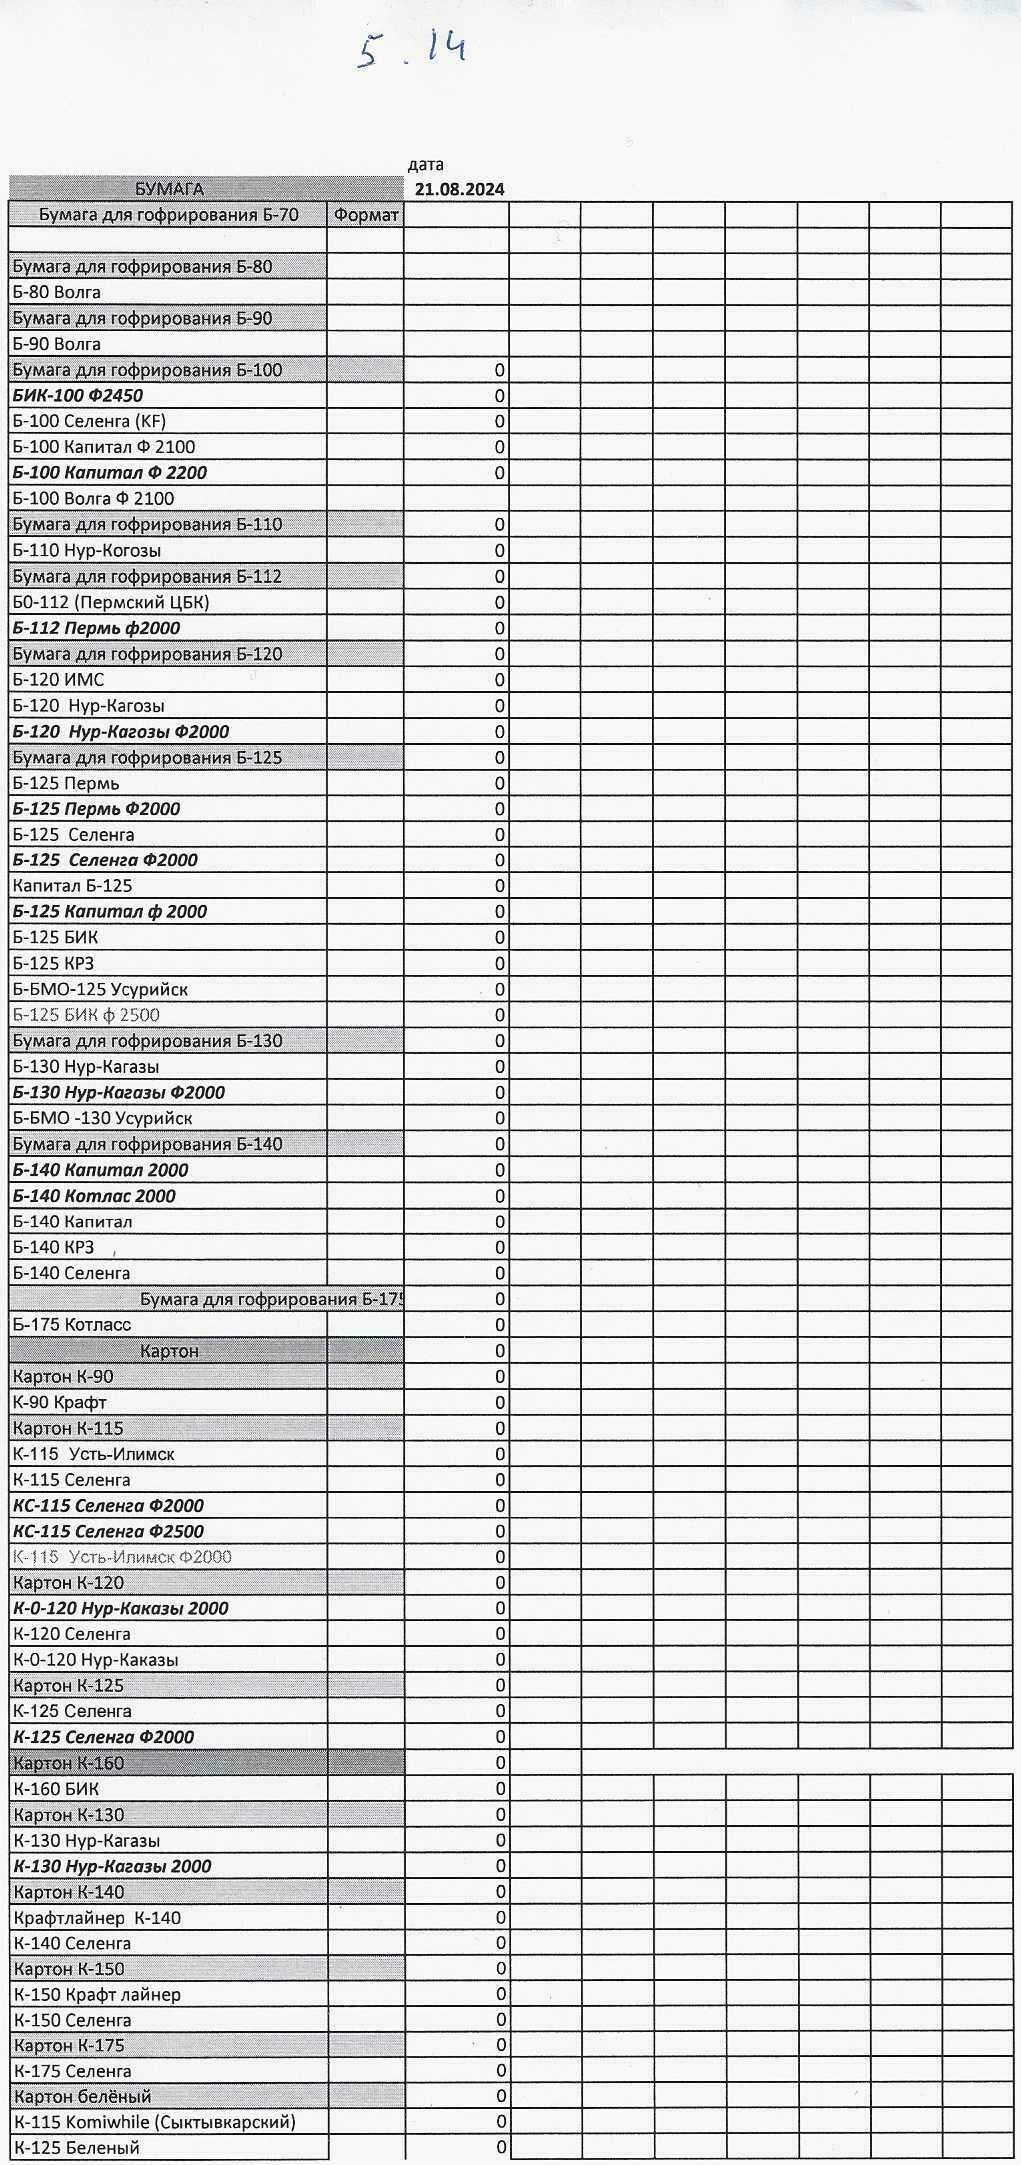
\includegraphics[height=0.94\textheight, width=0.94\textwidth, keepaspectratio]{Pics 1/5.14 файл бригадира по сырью_0001.jpg }
\end{center}
  \caption{Бланк учета сырья}
  \label{pic:5.14 файл бригадира по сырью_0001}
\end{figure}


\begin{figure}
\begin{center}
  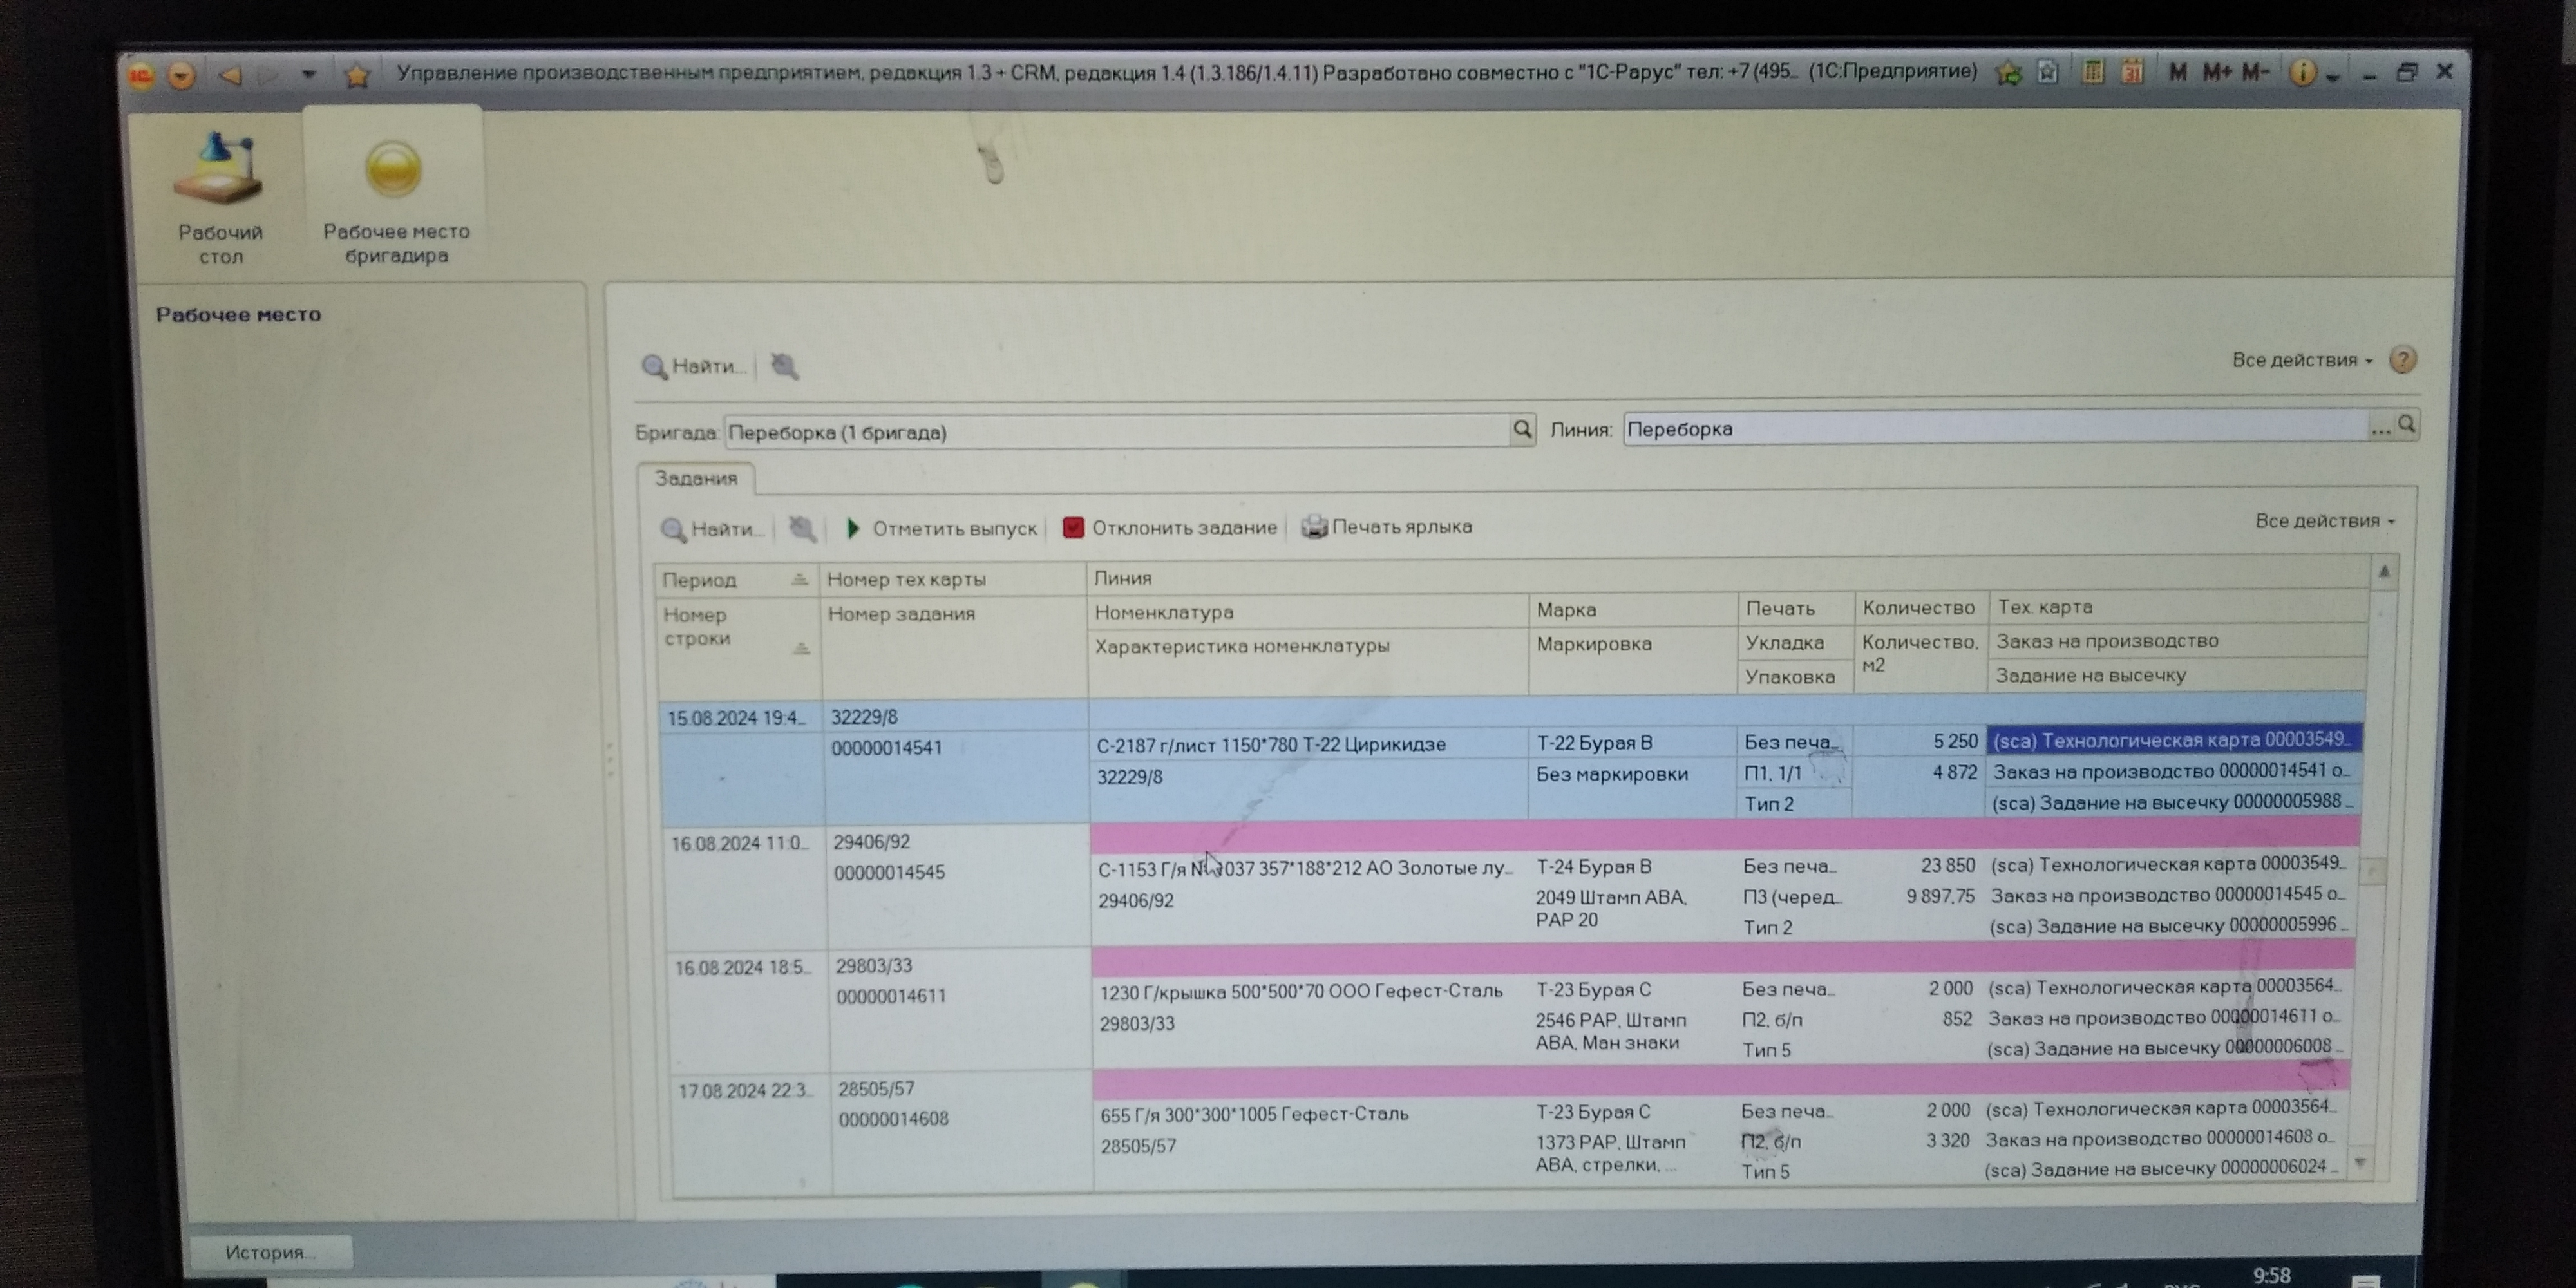
\includegraphics[height=0.94\textheight, width=0.94\textwidth, keepaspectratio]{Pics 1/7 рабочее место бригадира.jpg}
\end{center}
  \caption{Рабочее место бригадира линии в 1С:УПП}
  \label{pic:7 рабочее место бригадира}
\end{figure}

\begin{figure}
\begin{center}
  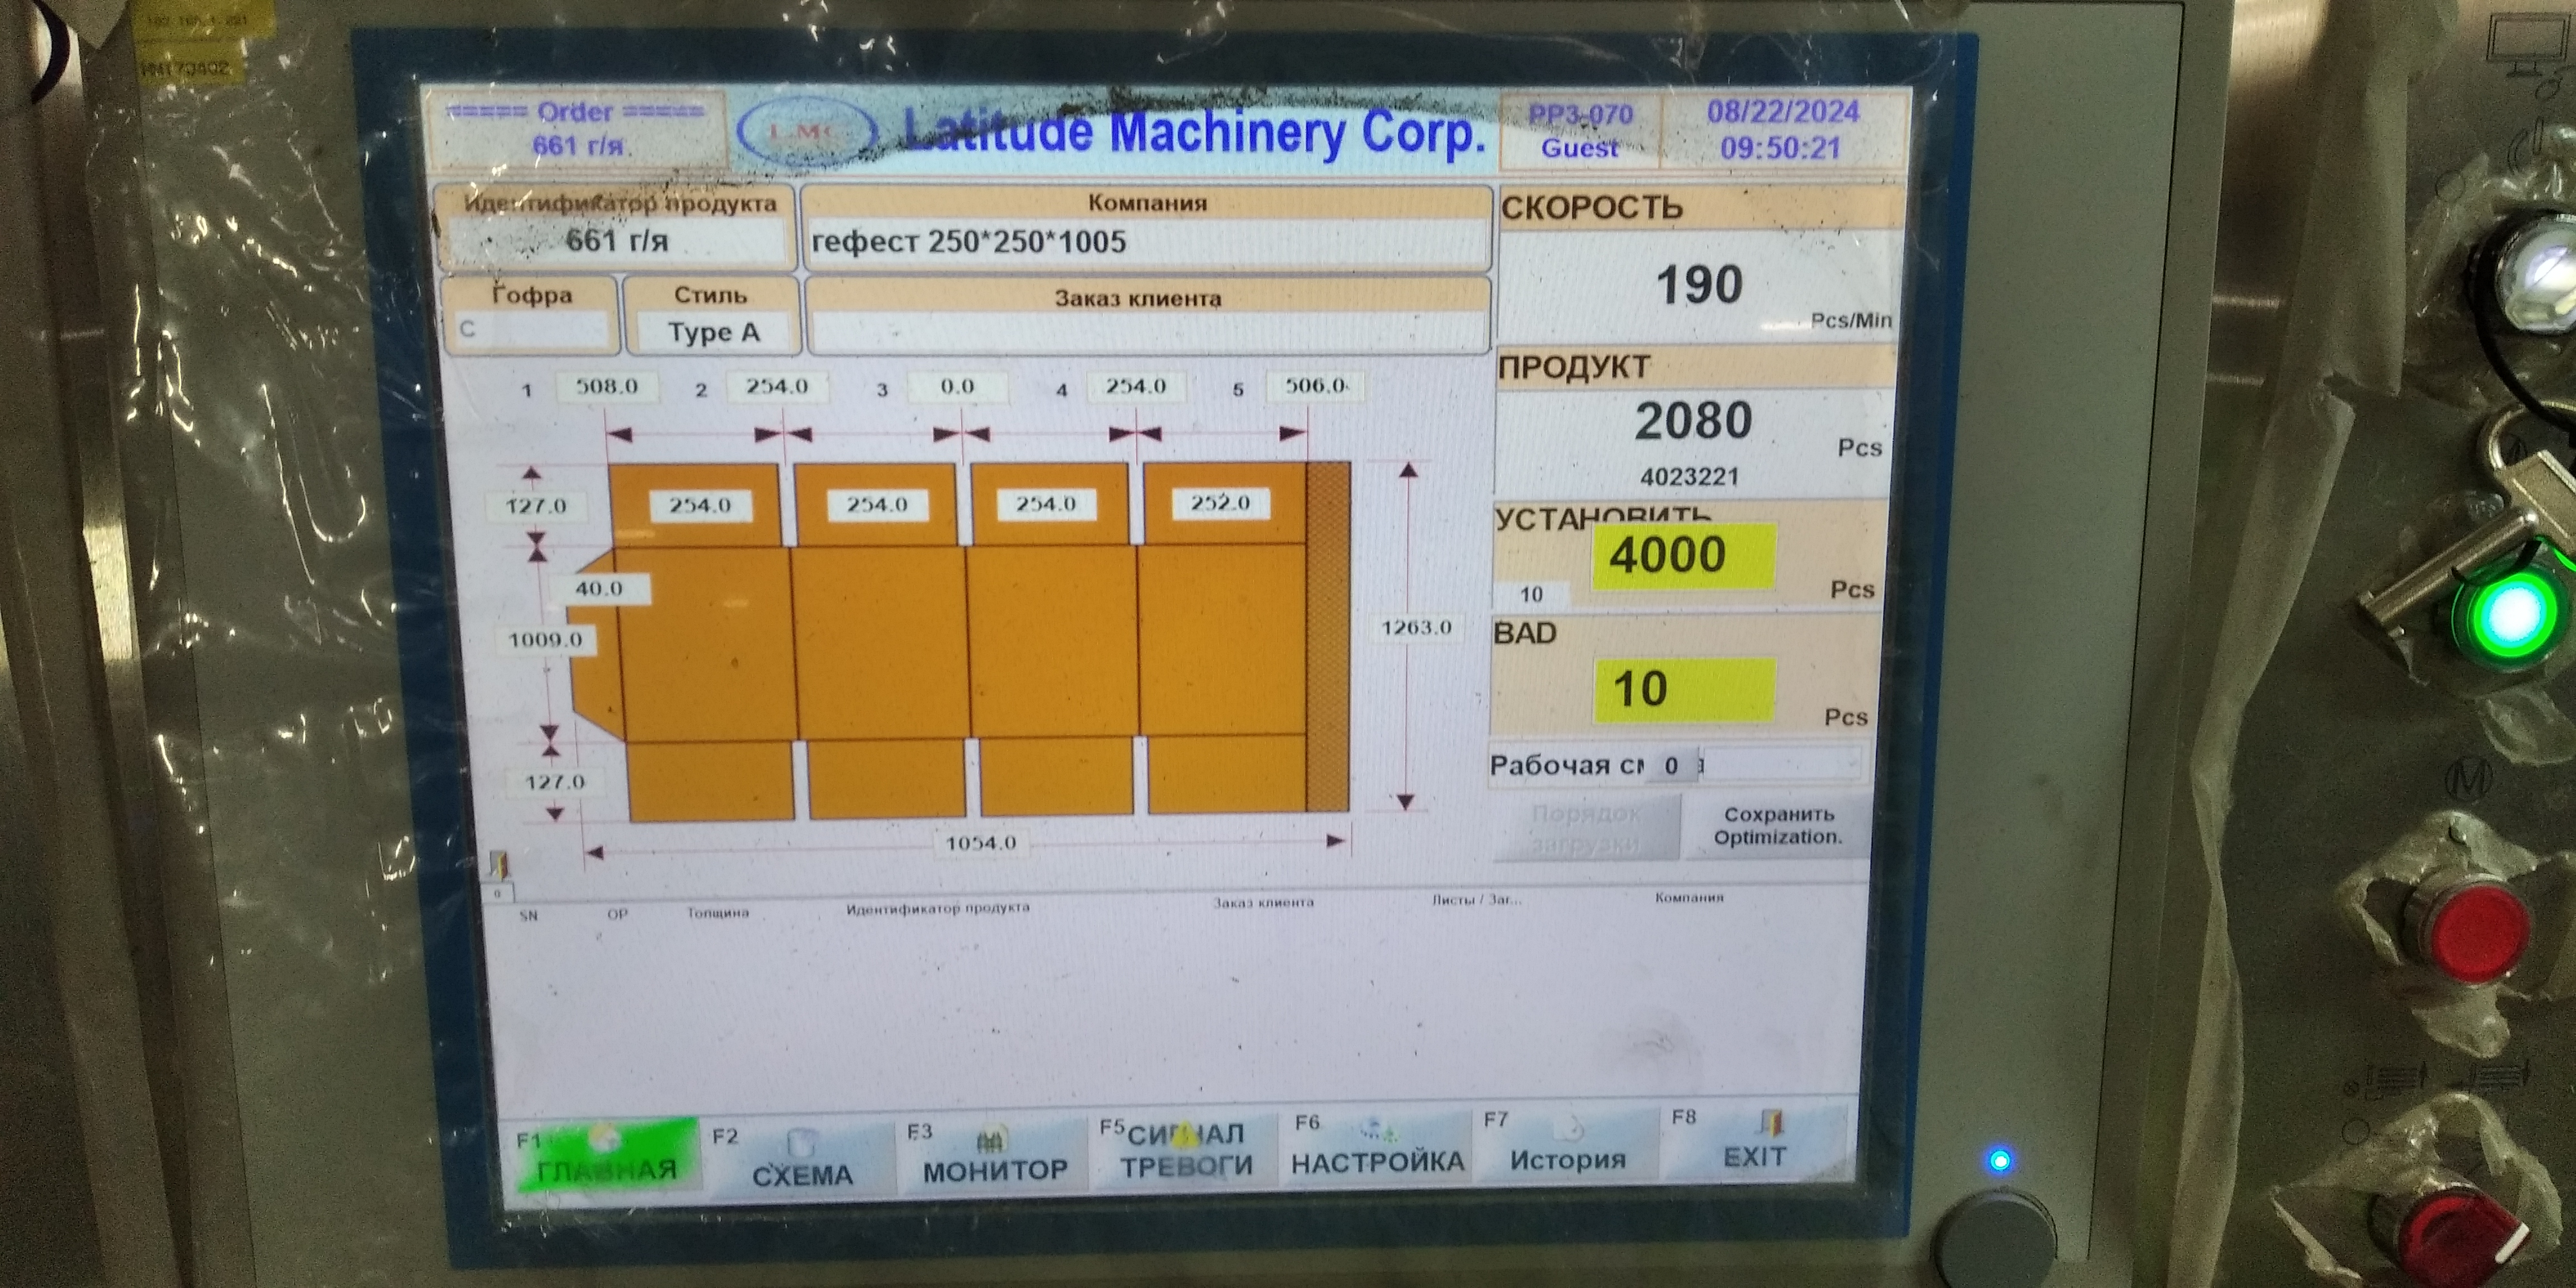
\includegraphics[height=0.94\textheight, width=0.94\textwidth, keepaspectratio]{Pics 1/7 Внесение данных из ТК в программу линии.jpg}
\end{center}
  \caption{Ввод данных на панели управления}
  \label{pic:7 Внесение данных из ТК в программу линии}
\end{figure}

\begin{figure}
\begin{center}
  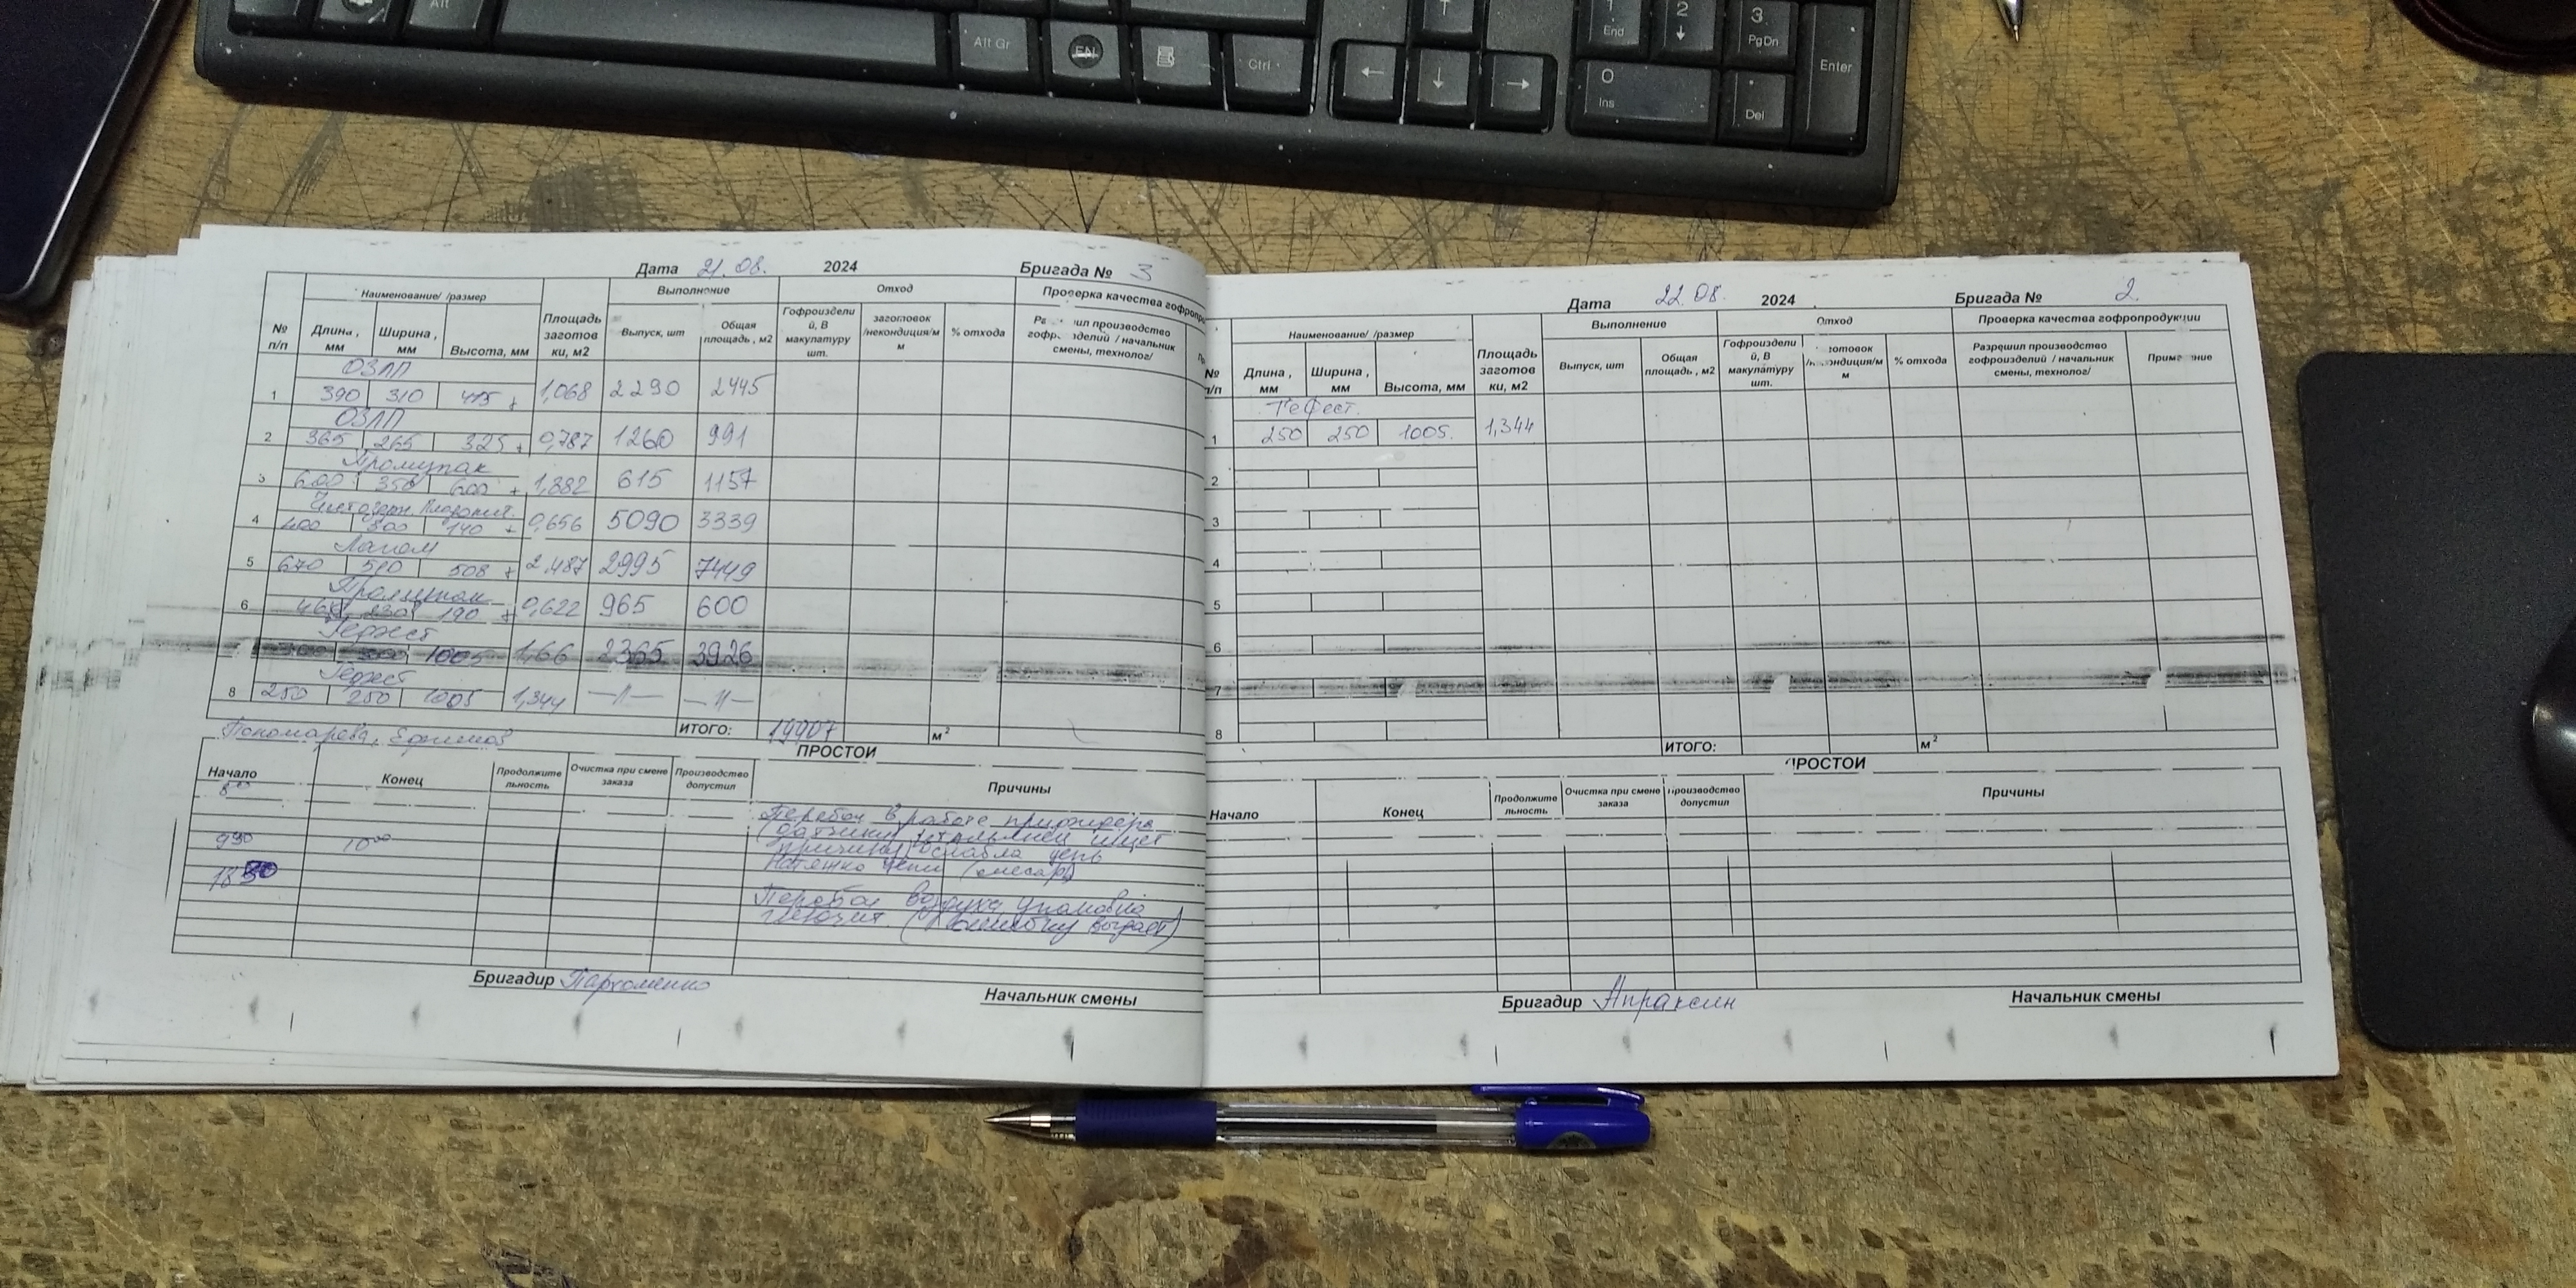
\includegraphics[height=0.94\textheight, width=0.94\textwidth, keepaspectratio]{Pics 1/7 журнал на линии 2.jpg}
\end{center}
  \caption{Журнал регистрации работ на линии переработки}
  \label{pic:7 журнал на линии 2}
\end{figure}

\begin{figure}
\begin{center}
  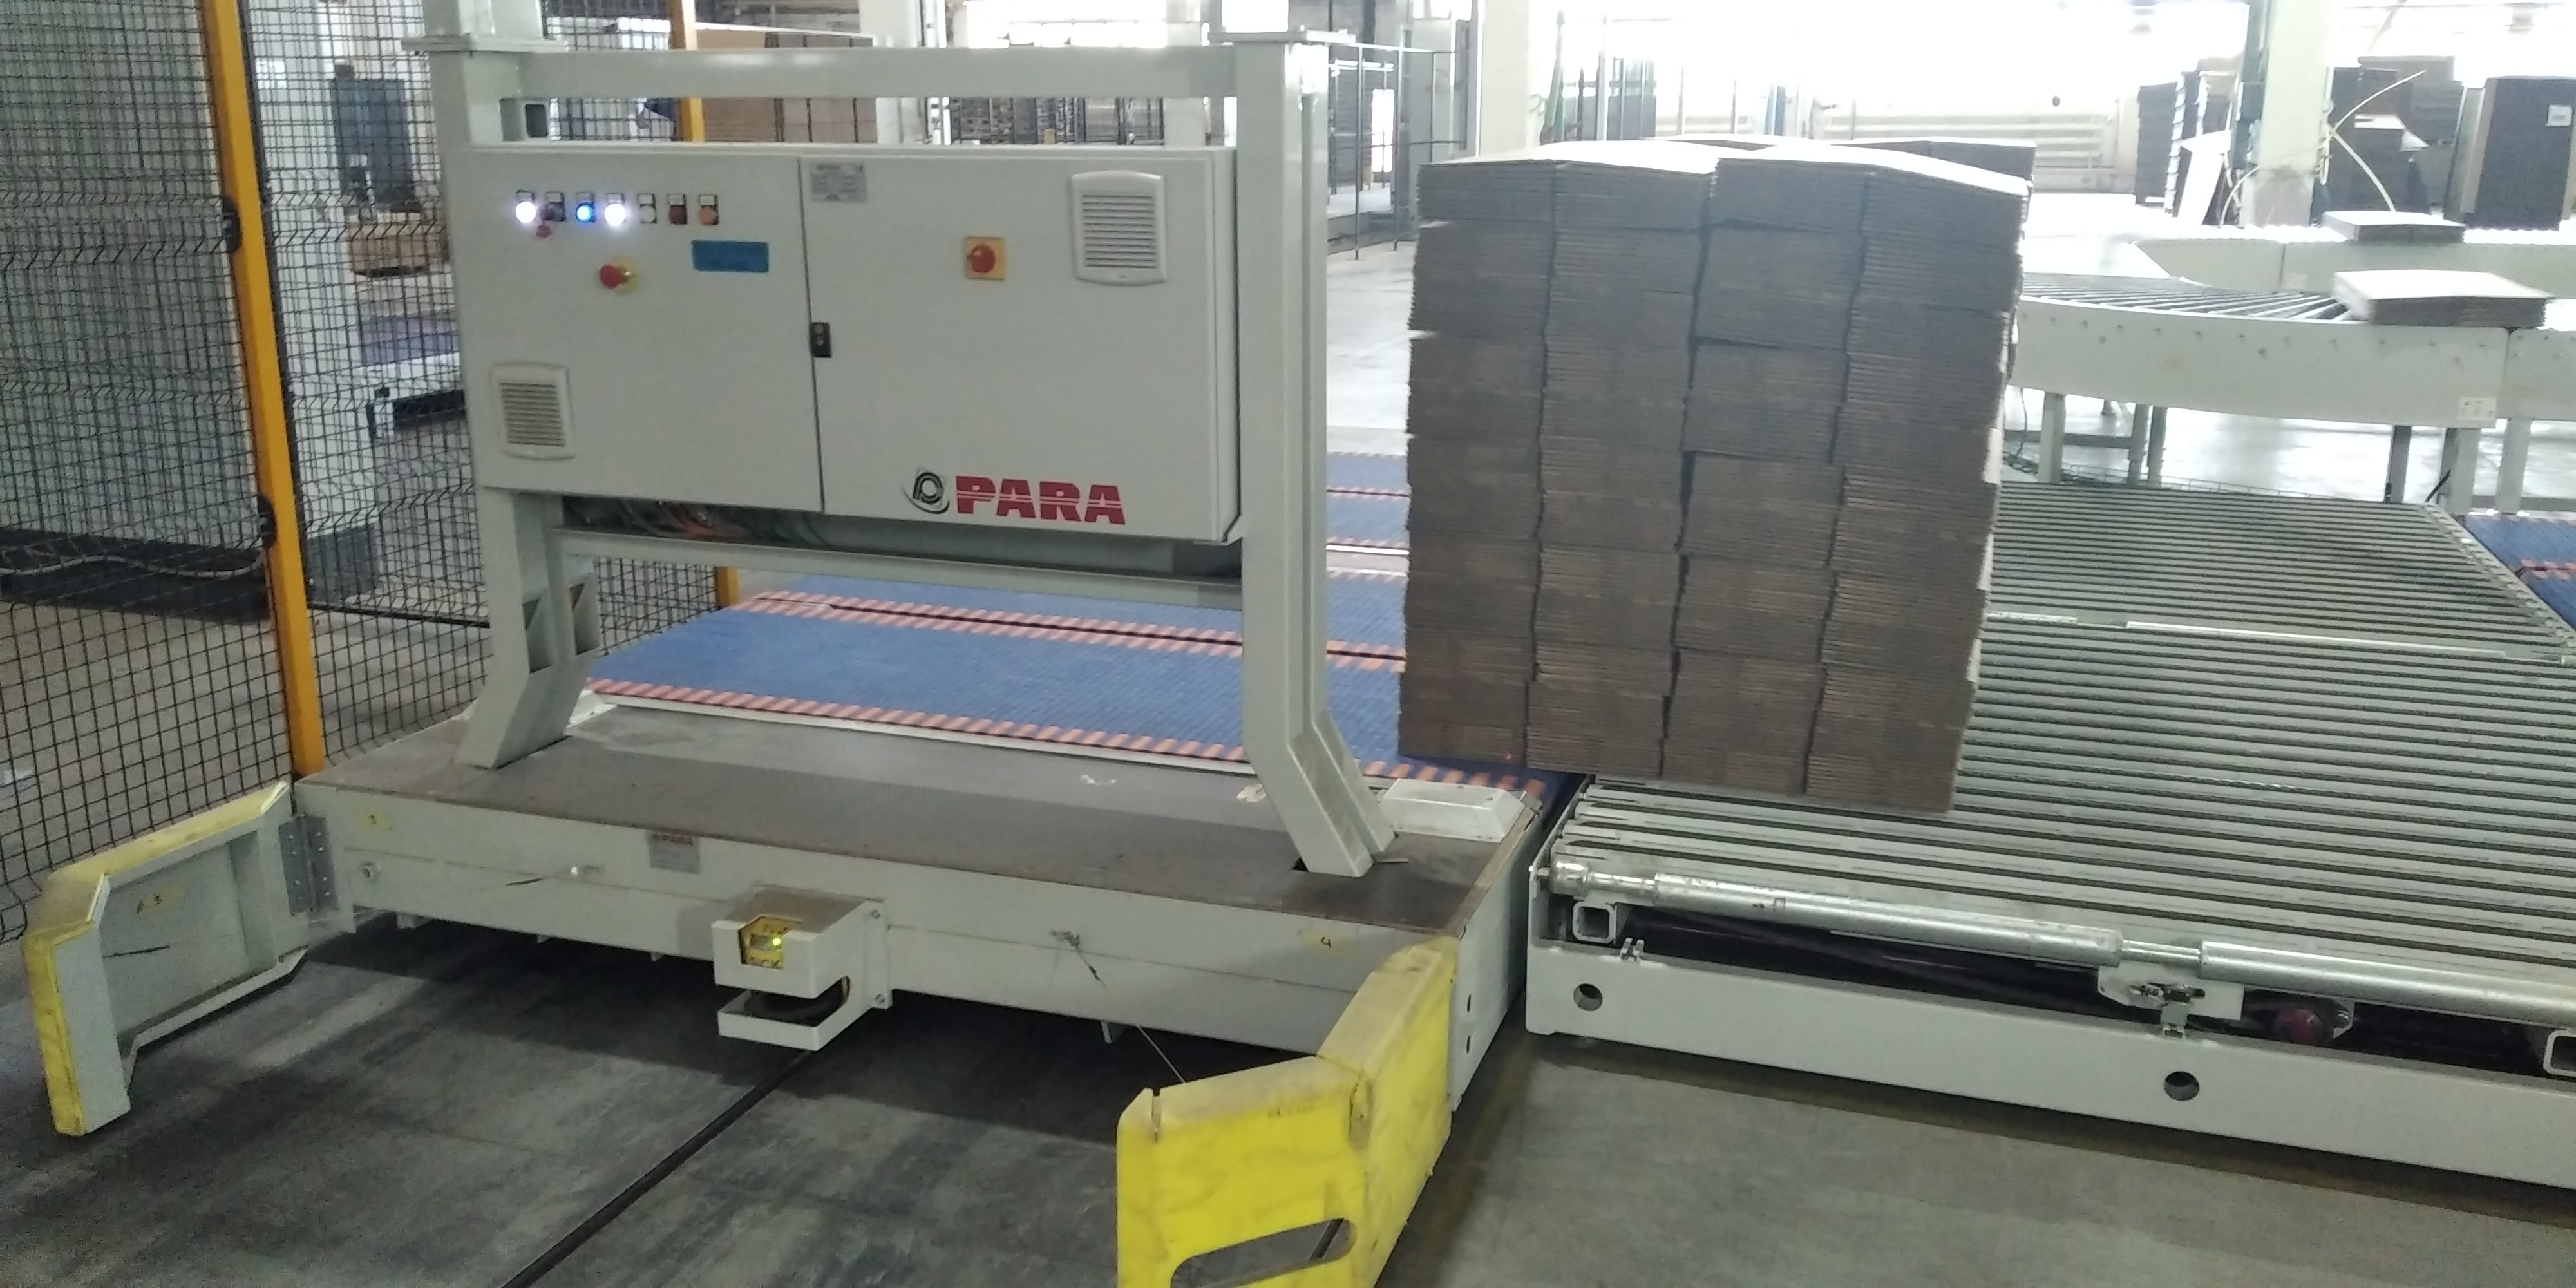
\includegraphics[height=0.94\textheight, width=0.94\textwidth, keepaspectratio]{Pics 1/7 перемещение паллет.jpg}
\end{center}
  \caption{Транспортная линия}
  \label{pic:7 перемещение паллет}
\end{figure}

%\clearpage

\begin{figure}
\begin{center}
  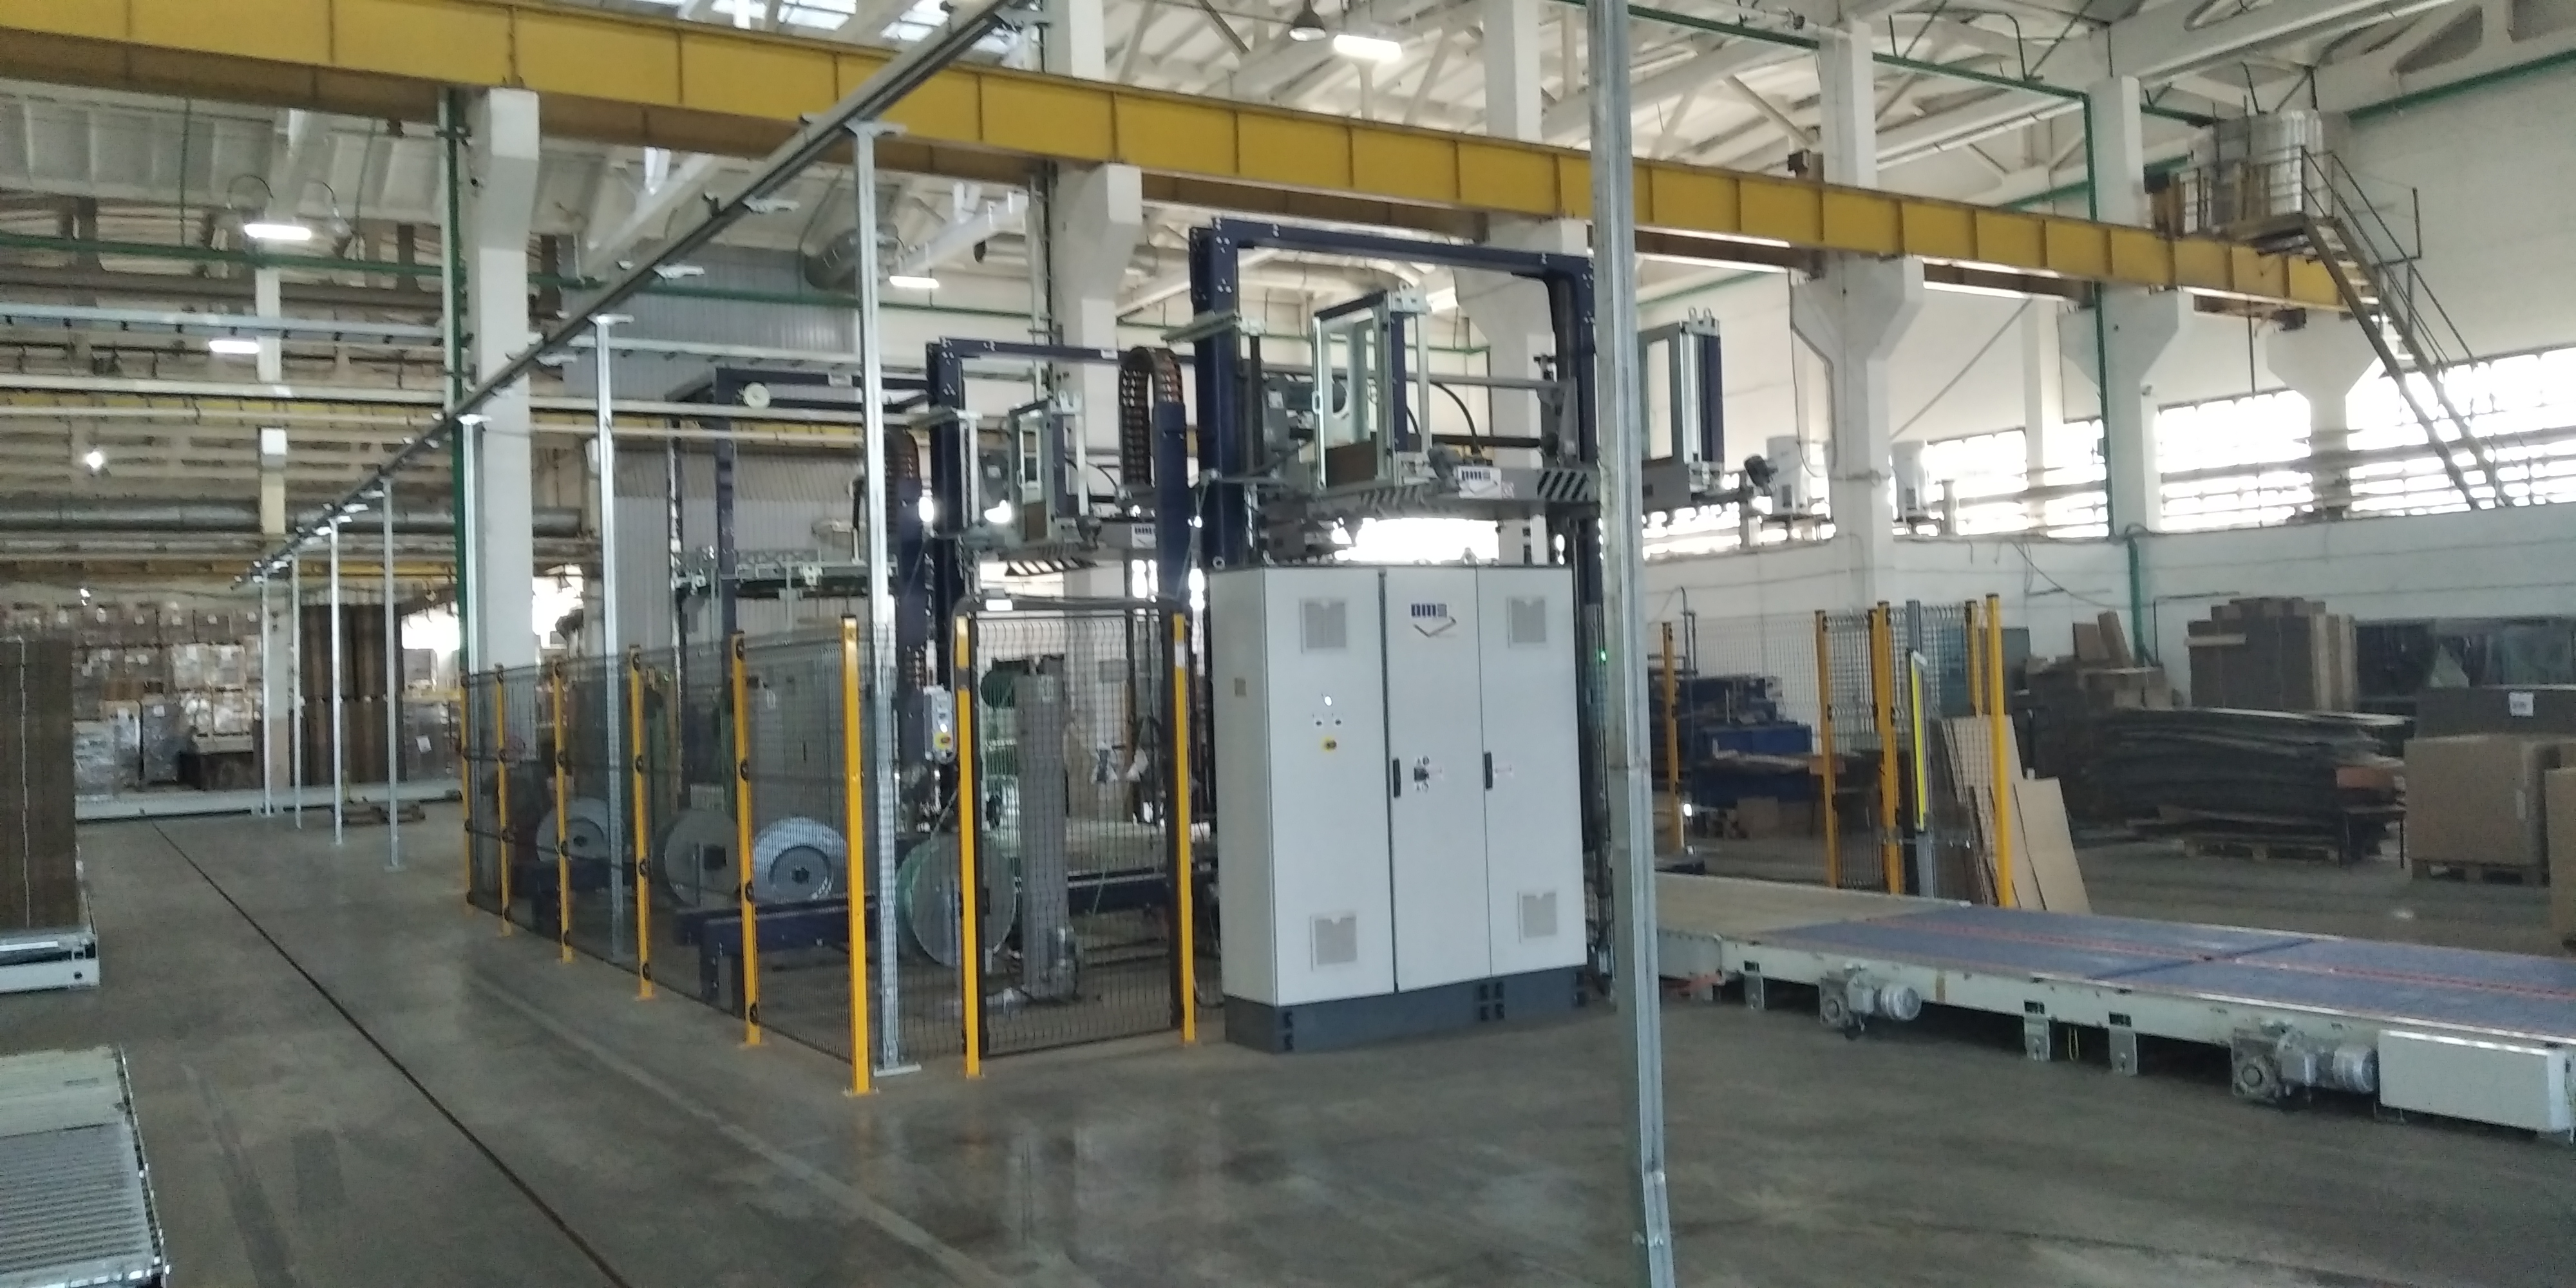
\includegraphics[height=0.94\textheight, width=0.94\textwidth, keepaspectratio]{Pics 1/7 Паллетировка.jpg}
\end{center}
  \caption{Линия автоматической паллетировки}
  \label{pic:7 Паллетировка}
\end{figure}

\begin{figure}
\begin{center}
  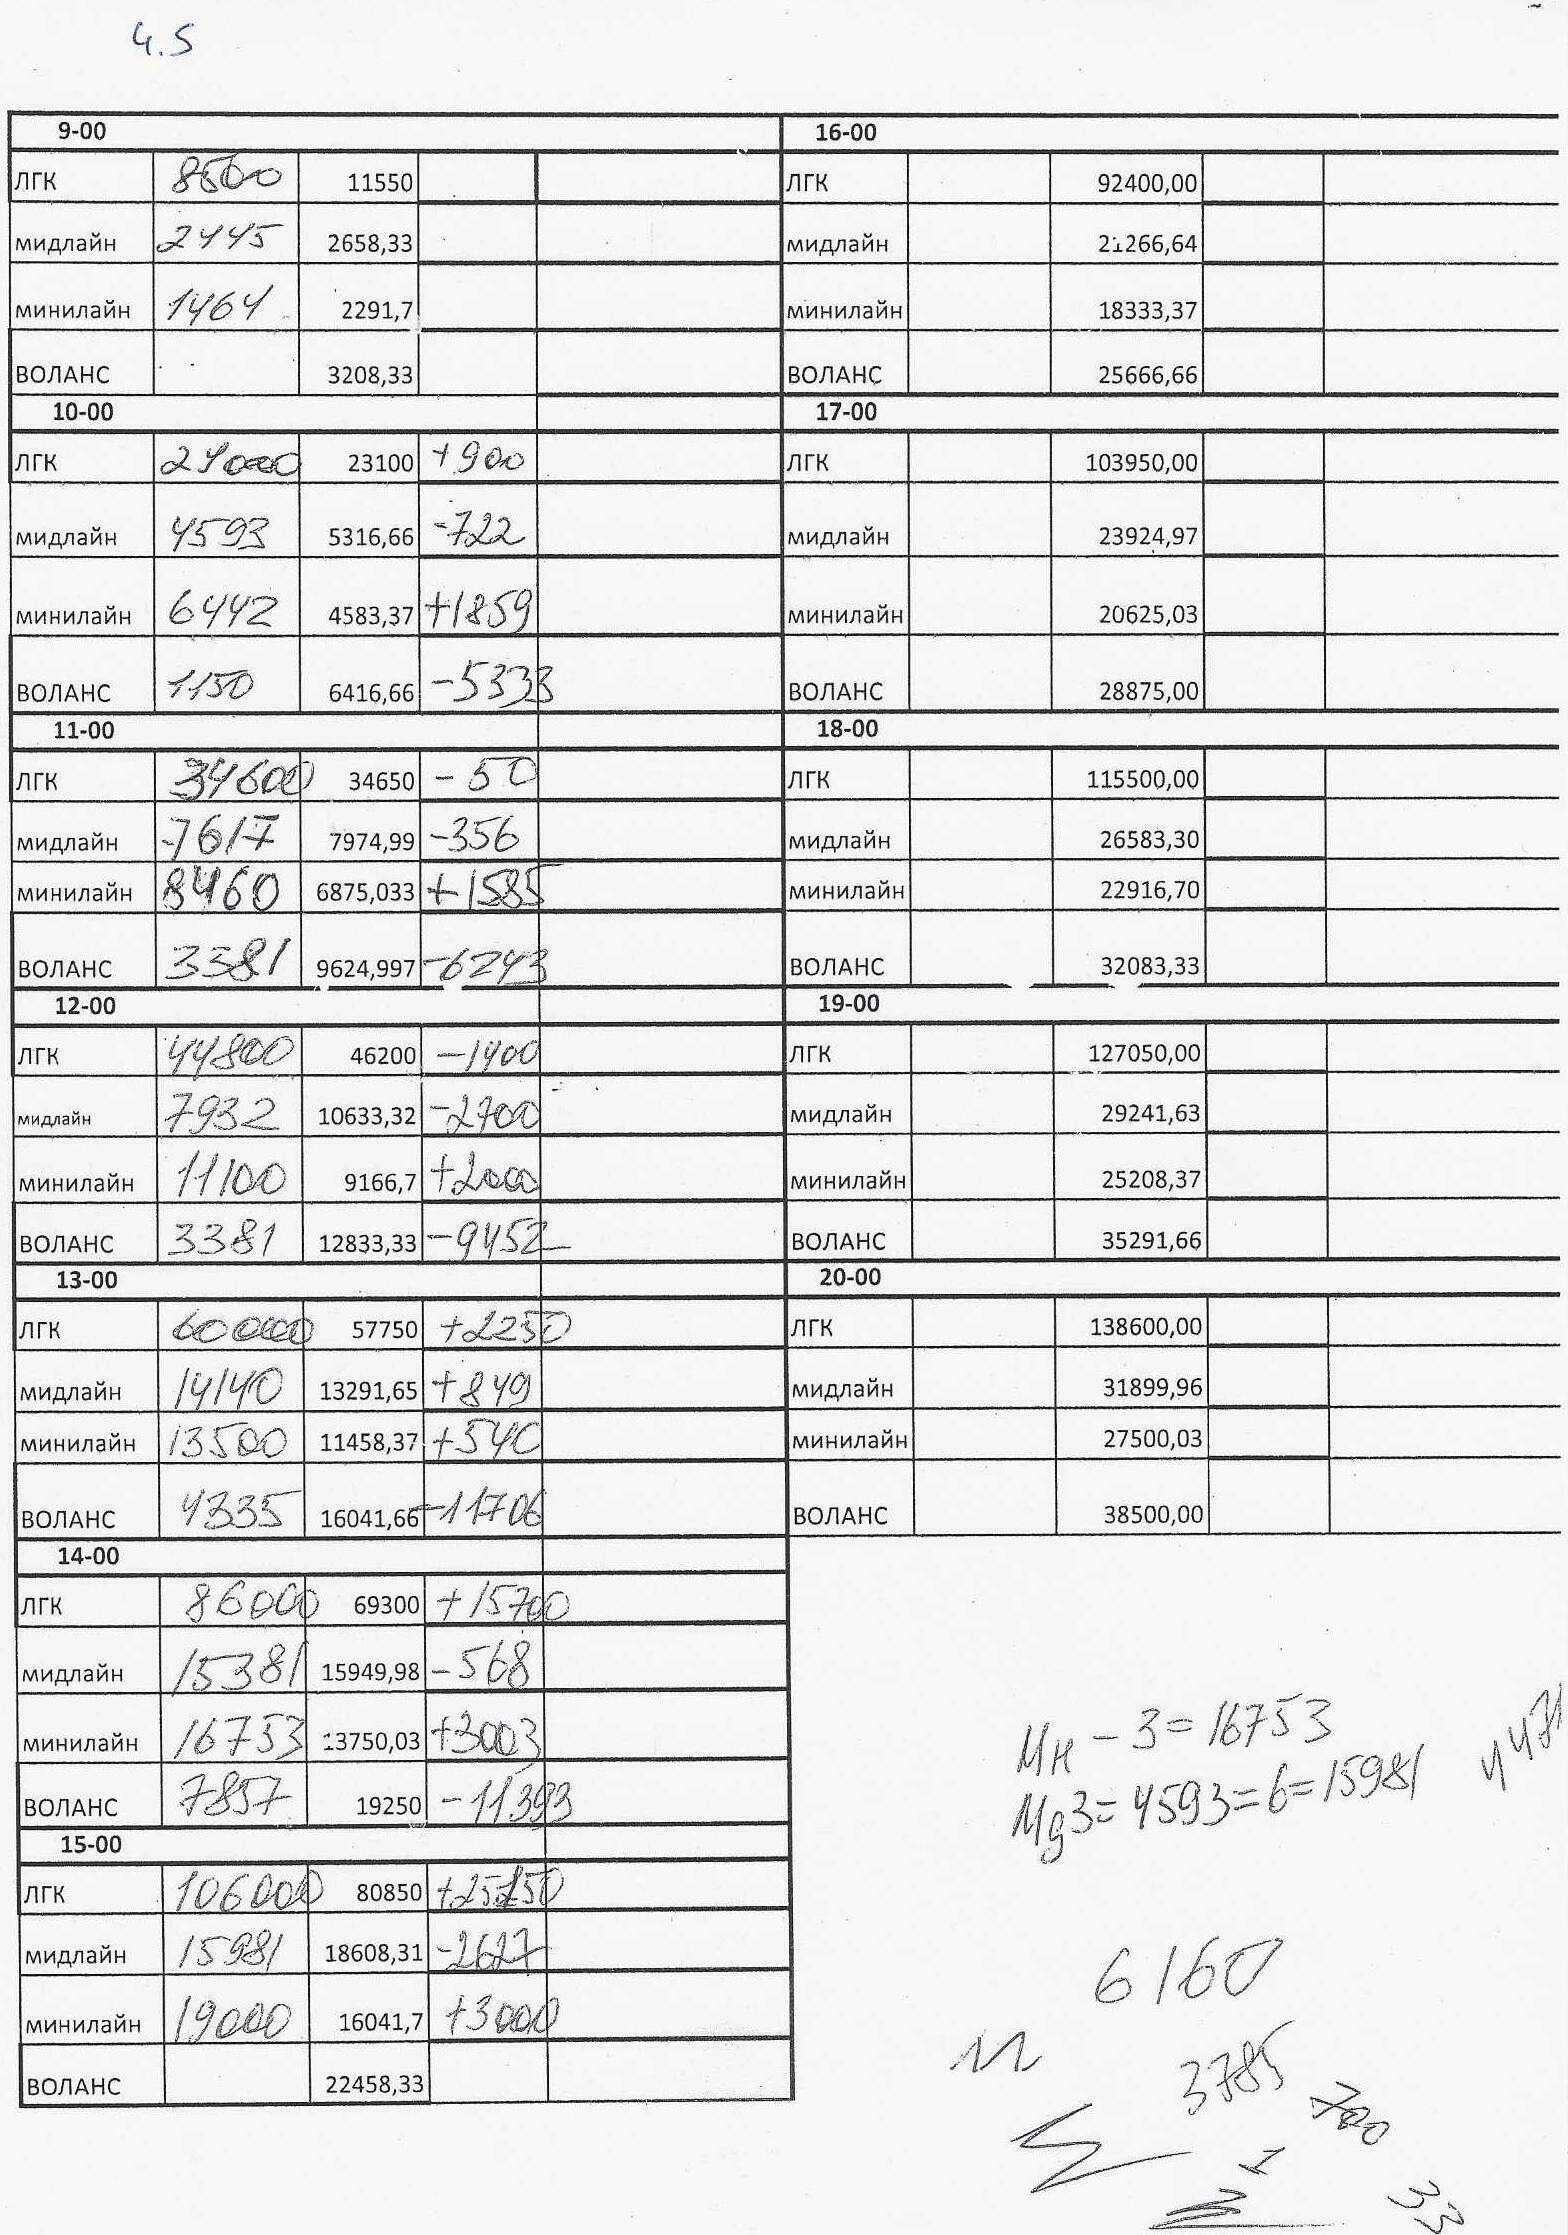
\includegraphics[height=0.94\textheight, width=0.94\textwidth, keepaspectratio]{Pics 1/4.5 почасовой отчет начсмены_0001.jpg}
\end{center}
  \caption{Отчет начальника смены}
  \label{pic:4.5 почасовой отчет начсмены_0001}
\end{figure}

\begin{figure}
\begin{center}
  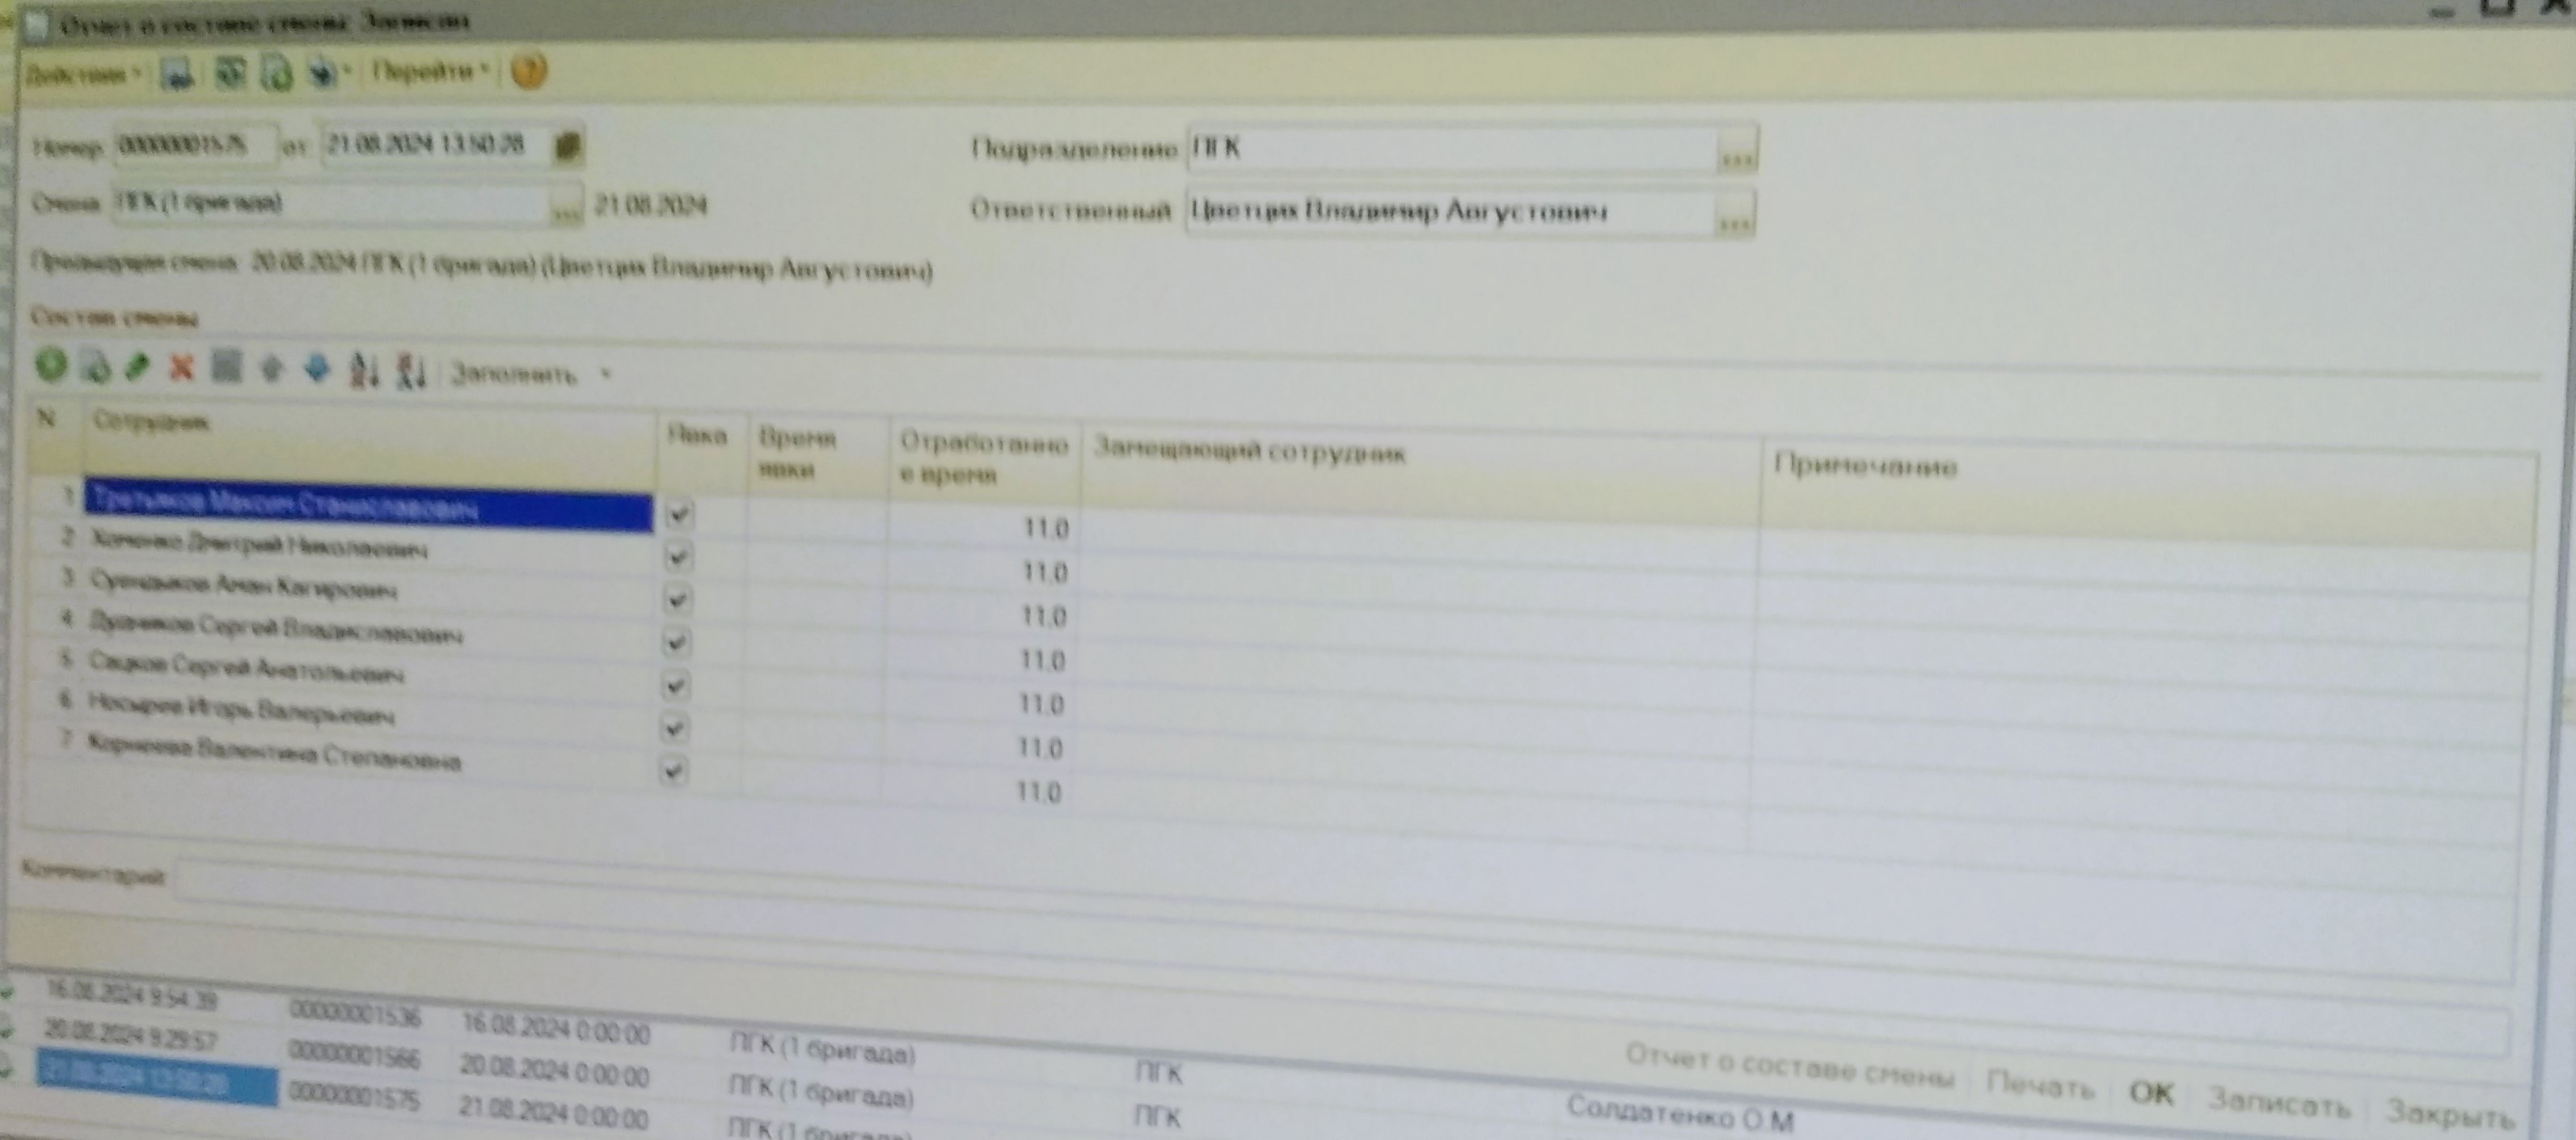
\includegraphics[height=0.94\textheight, width=0.94\textwidth, keepaspectratio]{Pics 1/4 табель смены в УПП.jpg}
\end{center}
  \caption{Табель в 1С:УПП}
  \label{pic:4 табель смены в УПП}
\end{figure}

\begin{figure}
\begin{center}
  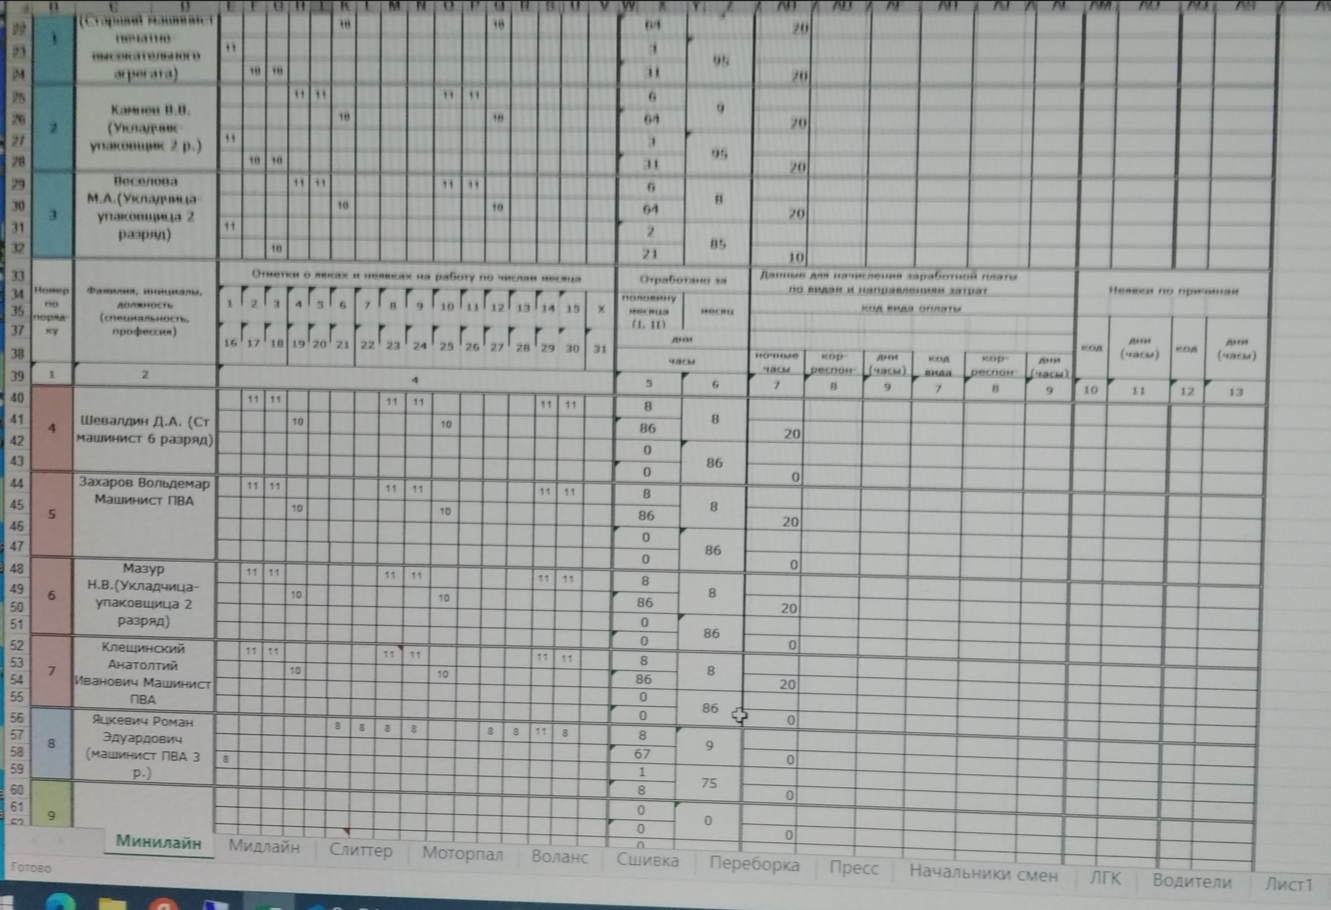
\includegraphics[height=0.94\textheight, width=0.94\textwidth, keepaspectratio]{Pics 1/4 рабочее время в эксель.png}
\end{center}
  \caption{Табель в MS Excel}
  \label{pic:4 рабочее время в эксель}
\end{figure}

\begin{figure}
\begin{center}
  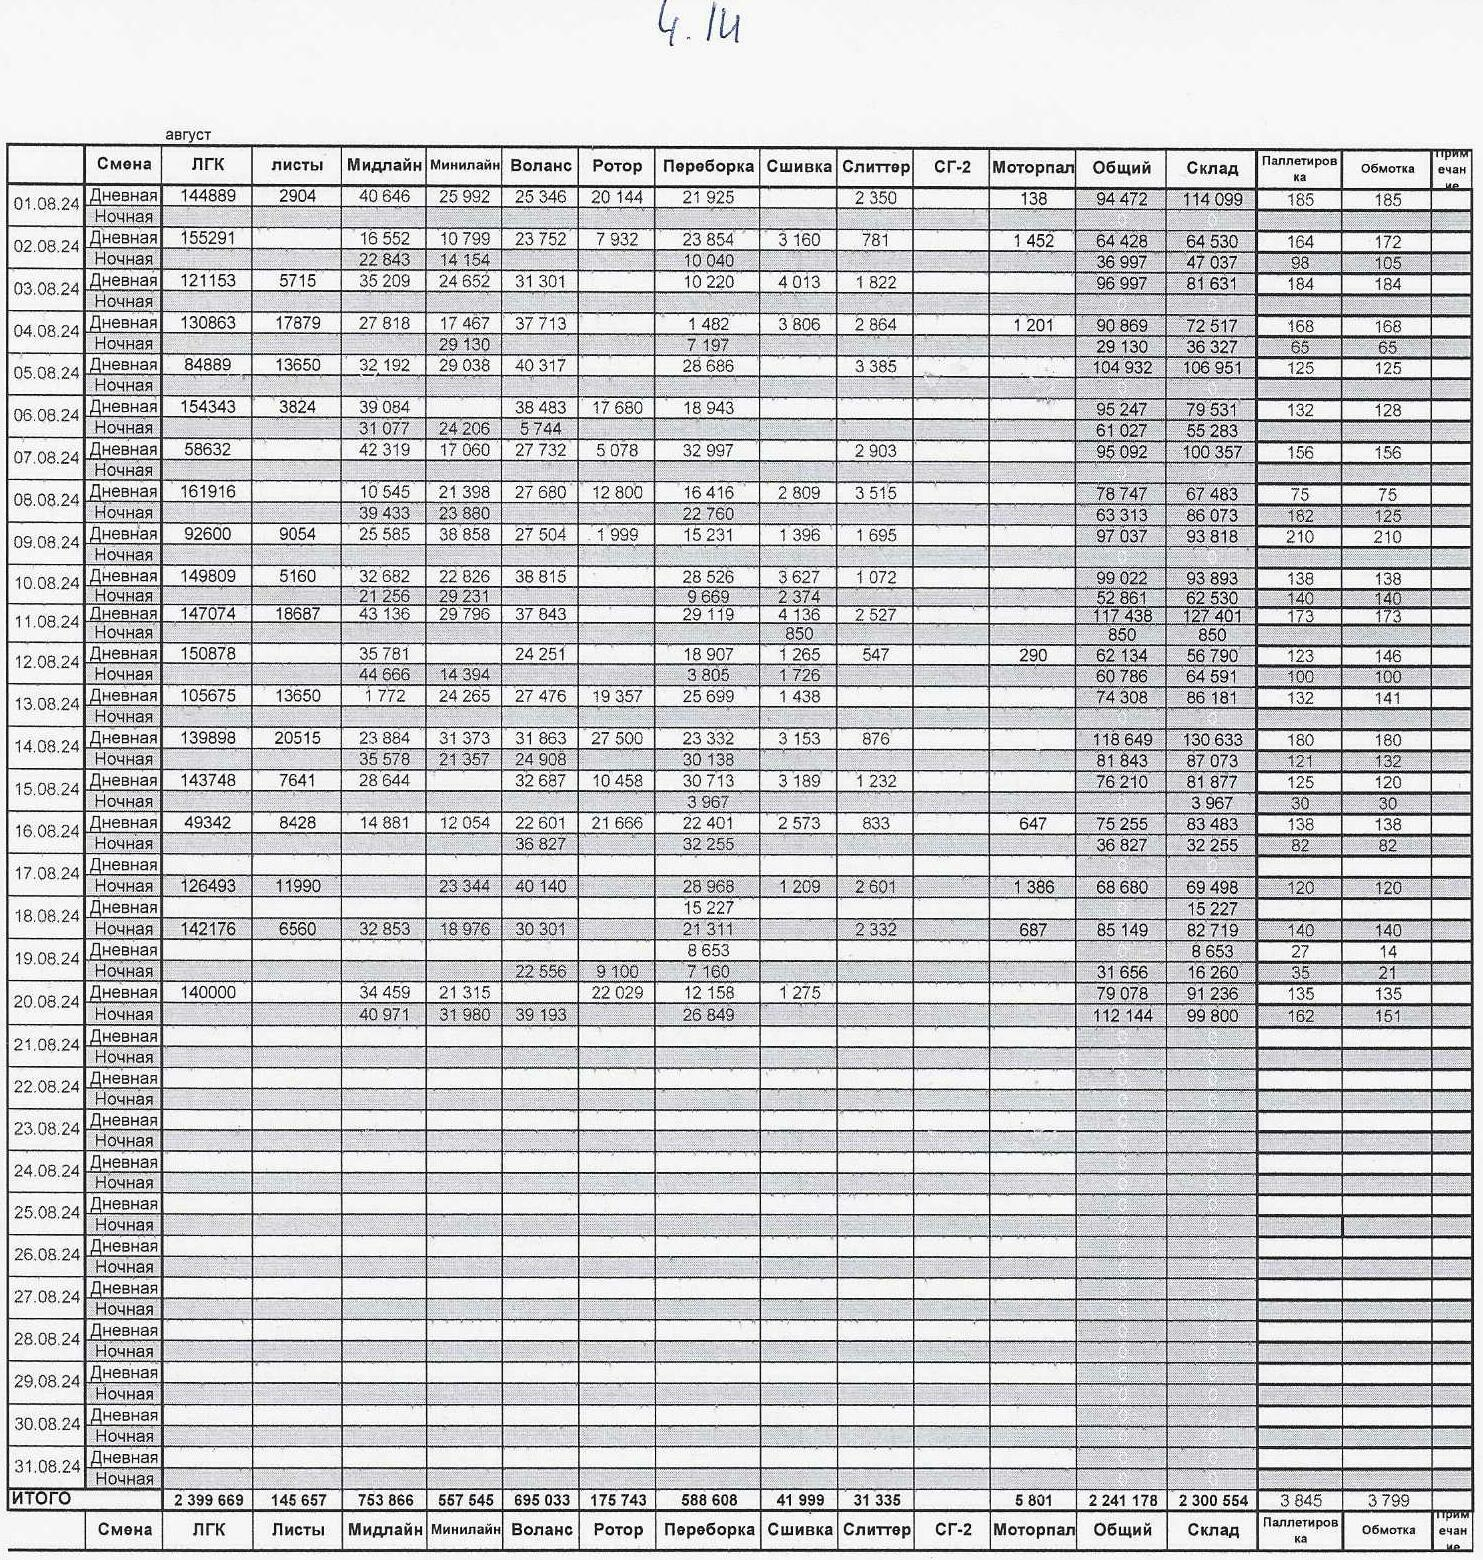
\includegraphics[height=0.94\textheight, width=0.94\textwidth, keepaspectratio]{Pics 1/4.14 сводная ведомость_0001.jpg}
\end{center}
  \caption{Сводная ведомость в MS Excel}
  \label{pic:4.14 сводная ведомость_0001}
\end{figure}
%Техники УВФ получают задание на производство около 15-00 и задание на ГА от коммерческого отдела (рис. \ref{pic:dd10}, \ref{pic:d15}). 
% ф. 13,14,15. 
%Техники УВФ начинают подготовку производства после получения заданий: готовят необходимые ТК по каждому заказу, готовят краску, указанную  в понтонах в ТК. 


%Мастер устно указывает машинисту линии, что делать согласно задания. Машинист находит свои задания в списке заданий,
% ф.22, 
%берет ТК и краску, подготовленные УВФ. При необходимости использования оснастки машинист находит ее на стеллажах. Машинист настраивает линию.

%Первые коробки, выпущенные с производственной линии, принимает контролер ОТК. 
%Контролер ОТК заполняет отчет по качеству и ставит подпись в бланке (рис. \ref{pic:f23}), который хранится в ОТК. Брак, внесенный в бланк, руками не пересчитывается, т.к. один контролер не успевает на все линии и заполняет по мере возможности. 

% Первые коробки принимает ОТК. Контролер ОТК заполняет и ставит подпись в бланке ф.23, который хранится в ОТК. Брак, внесенный в бланк, руками не пересчитывается, т.к. один контролер не успевает на все линии, заполняет по мере возможности. 

%Первый поддон с ГП отправляется на упаковку с биркой с ГА. Машинист линии упаковки ориентируется по бирке. 
%На упаковке машинист распечатывает ярлыки на ГП (рис. \ref{pic:a11}) из шаблона в MS Word
% базы ф.28 
%и размещает их на поддоне.

%На линиях переработки журналы по простоям машинисты не ведут. Мастер смены записывает в свой журнал все простои и замечания и передает их по смене (рис. \ref{pic:f29}).

%На основании рапортов мастер составляет отчет (рис. \ref{pic:a12}).

%Мастер забирает отчеты на выработке линий в 8.00 утра каждого рабочего дня и передает в БППП.
%Инженер БППП получает отчеты производства (рис. \ref{pic:d16}), отмечает в отчете заготовок (рис. \ref{pic:d14}). 
%В системе СБИС нет учета выработки по линии. Готовая продукция учитывается только по поступлению на склад.

%Каждый день менеджер отдела продаж получает отчеты производства в виде сканов в сетевой папке за прошедший день от БППП: отчет по заготовкам, остатки по ГП из СБИС (рис. \ref{pic:d21}).




\clearpage